% !TEX program = xelatex
% ============================================================
%  鹰眼长空 — 基于多平台协同的低空无人机智能监测系统
%  程序设计说明书  V1.0
% ============================================================
\documentclass[UTF8,12pt,oneside,a4paper,fontset=windows]{ctexart}

% ============================================================
%  鹰眼长空 — 程序设计说明书  排版导言区
%  编译：xelatex main.tex  (两遍，生成目录与交叉引用)
% ============================================================
\usepackage{geometry}
\geometry{left=2.6cm,right=2.6cm,top=2.6cm,bottom=2.4cm,headheight=15pt,footskip=1.0cm}

\usepackage{amsmath,amssymb,amsthm,bm}
\usepackage{graphicx}
\usepackage{float}
\usepackage{array,booktabs,longtable,tabularx,multirow,makecell}
\usepackage{xltabular}
\usepackage{enumitem}
\usepackage{xcolor}
\usepackage{tikz}
\usetikzlibrary{arrows.meta,positioning,shapes.geometric,shapes.misc,shapes.symbols,fit,backgrounds,calc,chains,decorations.pathreplacing,decorations.markings,patterns,matrix}
\usepackage{caption}
\usepackage{fancyhdr}
\usepackage{listings}
\usepackage[most]{tcolorbox}
\usepackage[hidelinks,bookmarksnumbered,bookmarksopen]{hyperref}
\usepackage{url}

% ---------- 黑白配色（白底黑字） ----------
\definecolor{bwtext}{gray}{0}
\definecolor{bwgray}{gray}{0.35}
\definecolor{bwlight}{gray}{0.92}
\definecolor{bwfill}{gray}{0.96}
\color{black}

% ---------- 字体（SimHei 无粗体，启用伪粗体） ----------
\setCJKmainfont[AutoFakeBold=2.4]{SimSun}
\setCJKsansfont[AutoFakeBold=2.4]{SimHei}
\setCJKmonofont[AutoFakeBold=2.0]{SimSun}

% ---------- 标题格式 ----------
\ctexset{
  section = {
    format = \Large\heiti,
    name = {,},
    number = \arabic{section},
    aftername = \hspace{0.7em},
    beforeskip = 1.2ex plus .2ex,
    afterskip = 1.0ex plus .2ex,
  },
  subsection = {
    format = \large\heiti,
    number = \arabic{section}.\arabic{subsection},
    aftername = \hspace{0.7em},
    beforeskip = 1.0ex plus .2ex,
    afterskip = 0.8ex plus .2ex,
  },
  subsubsection = {
    format = \normalsize\heiti,
    number = \arabic{section}.\arabic{subsection}.\arabic{subsubsection},
    aftername = \hspace{0.6em},
    beforeskip = 0.8ex plus .2ex,
    afterskip = 0.6ex plus .2ex,
  },
}

% ---------- 图表编号：章-序 ----------
\counterwithin{figure}{section}
\counterwithin{table}{section}
\counterwithin{equation}{section}
\renewcommand{\thefigure}{\thesection-\arabic{figure}}
\renewcommand{\thetable}{\thesection-\arabic{table}}
\renewcommand{\theequation}{\thesection-\arabic{equation}}
\captionsetup{font=small,labelsep=quad,justification=centering}
\captionsetup[table]{skip=4pt}
\captionsetup[figure]{skip=4pt}
\renewcommand{\figurename}{图}
\renewcommand{\tablename}{表}
\renewcommand{\lstlistingname}{代码}

% ---------- 页眉页脚 ----------
\pagestyle{fancy}
\fancyhf{}
\fancyhead[L]{\small\songti 鹰眼长空 — 低空无人机智能监测系统}
\fancyhead[R]{\small\songti 程序设计说明书}
\fancyfoot[C]{\small\thepage}
\renewcommand{\headrulewidth}{0.4pt}
\renewcommand{\footrulewidth}{0pt}
\fancypagestyle{plain}{\fancyhf{}\fancyfoot[C]{\small\thepage}\renewcommand{\headrulewidth}{0pt}}

% ---------- 列表 ----------
\setlist[itemize]{leftmargin=2em,itemsep=2pt,topsep=3pt,parsep=0pt}
\setlist[enumerate]{leftmargin=2.4em,itemsep=2pt,topsep=3pt,parsep=0pt}

% ---------- 代码清单 ----------
\lstdefinestyle{py}{
  language=Python,
  basicstyle=\ttfamily\footnotesize,
  keywordstyle=\bfseries,
  commentstyle=\color{bwgray},
  stringstyle=\color{black},
  frame=single,
  rulecolor=\color{black!40},
  framexleftmargin=10pt,
  numbers=left,
  numberstyle=\tiny\color{bwgray},
  numbersep=6pt,
  breaklines=true,
  breakatwhitespace=false,
  columns=fullflexible,
  keepspaces=true,
  showstringspaces=false,
  tabsize=4,
  aboveskip=6pt,
  belowskip=6pt,
  xleftmargin=22pt,
  extendedchars=true,
  inputencoding=utf8,
}
\lstdefinestyle{json}{
  basicstyle=\ttfamily\footnotesize,
  frame=single,
  rulecolor=\color{black!40},
  breaklines=true,
  columns=fullflexible,
  showstringspaces=false,
  aboveskip=6pt,
  belowskip=6pt,
}
\lstdefinestyle{sh}{
  language=bash,
  basicstyle=\ttfamily\footnotesize,
  frame=single,
  rulecolor=\color{black!40},
  breaklines=true,
  columns=fullflexible,
  showstringspaces=false,
  aboveskip=6pt,
  belowskip=6pt,
}
\lstset{style=py}

% ---------- 提示框（黑白） ----------
\newtcolorbox{notebox}[1][]{
  enhanced,
  colback=white,
  colframe=black!55,
  boxrule=0.5pt,
  arc=2pt,
  left=6pt,right=6pt,top=4pt,bottom=4pt,
  fonttitle=\bfseries\heiti,
  title=#1,
  breakable,
}

% ---------- 插图配色（正文仍为黑白） ----------
\definecolor{cA}{RGB}{222,235,249}   % 蓝
\definecolor{cB}{RGB}{228,243,231}   % 绿
\definecolor{cC}{RGB}{252,241,222}   % 橙
\definecolor{cD}{RGB}{238,240,245}   % 灰
\definecolor{cLine}{RGB}{58,78,104}  % 深蓝灰描边
\definecolor{cLbl}{RGB}{45,45,45}

% ---------- TikZ 统一风格 ----------
\tikzset{
  base/.style   = {draw=cLine, line width=0.5pt, fill=cA, align=center,
                   font=\small, inner sep=3pt, minimum height=8mm, text=black},
  proc/.style   = {base, rectangle, rounded corners=1.5pt, minimum width=26mm},
  deci/.style   = {base, diamond, aspect=2.2, inner sep=1pt, minimum width=20mm,
                   minimum height=9mm, font=\footnotesize, fill=cC},
  term/.style   = {base, rectangle, rounded corners=9pt, minimum width=24mm, fill=cB},
  data/.style   = {base, trapezium, trapezium left angle=72, trapezium right angle=108,
                   text width=26mm, inner sep=3pt, fill=cD},
  doc/.style    = {base, signal, signal to=east, minimum width=26mm, inner sep=5pt, fill=cD},
  layer/.style  = {draw=cLine, line width=0.7pt, fill=cD!35, inner sep=8pt,
                   rounded corners=3pt},
  grp/.style    = {draw=cLine!80, line width=0.5pt, rounded corners=2pt, inner sep=7pt, fill=white},
  arr/.style    = {-{Stealth[length=2.2mm]}, line width=0.5pt, draw=cLine},
  darr/.style   = {-{Stealth[length=2.2mm]}, line width=0.4pt, draw=cLine, dashed},
  busr/.style   = {-{Stealth[length=2.2mm]}, line width=1.0pt, draw=cLine},
  lbl/.style    = {font=\scriptsize, inner sep=1.5pt, fill=white, text=black},
}

% ---------- 自定义命令 ----------
\newcommand{\code}[1]{\texttt{\detokenize{#1}}}
\newcommand{\file}[1]{\path{#1}}   % 路径使用 url 宏包，可在 / 处断行
\def\UrlBreaks{\do\/\do\_\do\.\do\-}
\newcommand{\term}[1]{\textbf{#1}}
\renewcommand{\arraystretch}{1.25}
\setcounter{tocdepth}{2}
\renewcommand{\topfraction}{0.85}
\renewcommand{\bottomfraction}{0.7}
\renewcommand{\textfraction}{0.12}
\renewcommand{\floatpagefraction}{0.75}
\setlength{\parindent}{2em}
\setlength{\parskip}{0.35ex}
\setlength{\emergencystretch}{2.5em}
\tolerance=1500


% ---------- 截图标注点（第 11 章使用） ----------
\tikzset{
  hmark/.style={circle, draw=white, line width=0.9pt, fill=cLine,
               text=white, font=\bfseries\scriptsize, inner sep=1.4pt,
               minimum size=4.6mm, opacity=0.96, text opacity=1},
}
\newcommand{\hotspot}[3]{\node[hmark] at (#2,#3) {#1};}
\newcommand{\cn}[1]{\textcircled{\footnotesize #1}}


\hypersetup{
  pdftitle={鹰眼长空 — 低空无人机智能监测系统 程序设计说明书},
  pdfauthor={鹰眼长空项目组},
  pdfsubject={软件设计文档},
  pdfkeywords={无人机监测; 双目立体视觉; 轨迹重建; 程序设计},
}

\begin{document}

% ==================== 封面 ====================
\begin{titlepage}
\thispagestyle{empty}
\centering
\vspace*{2.0cm}

{\heiti\zihao{2} 鹰眼长空}\\[6pt]
{\heiti\zihao{3} 基于多平台协同的低空无人机智能监测系统}\\[2.2cm]

{\heiti\zihao{1} 程序设计说明书}\\[10pt]
{\heiti\zihao{3} V1.0}\\[2.6cm]

\begin{tcolorbox}[width=0.74\textwidth, colback=white, colframe=black,
                  boxrule=0.8pt, arc=0pt, left=18pt, right=18pt, top=12pt, bottom=12pt]
\renewcommand{\arraystretch}{1.7}
\zihao{5}
\begin{tabularx}{\linewidth}{@{}>{\heiti}l@{\hspace{1.5em}}X@{}}
软件名称 & 鹰眼长空 — 低空无人机智能监测系统 \\
版本号   & V1.0 \\
文档类型 & 程序设计说明书（软件设计文档） \\
开发语言 & Python 3.11（后端）、JavaScript ES6（前端） \\
完成日期 & 2026 年 10 月 \\
\end{tabularx}
\end{tcolorbox}

\vfill
{\zihao{5} 二〇二六年十月}
\end{titlepage}

% ==================== 目录 ====================
\clearpage
\pagenumbering{Roman}
\renewcommand{\contentsname}{目\quad 录}
\tableofcontents
\clearpage

% ==================== 正文 ====================
\pagenumbering{arabic}
% ============================================================
%  第一章  引言
% ============================================================
\section{引言}

\subsection{编写目的}

本文档是“鹰眼长空”（低空无人机智能监测系统，版本 V1.0）的程序设计说明书，用于完整描述该软件的系统架构、程序流程、模块划分、核心算法、数据结构与接口约定，为软件的开发维护、功能扩展、测试验收以及软件著作权登记提供技术依据。

文档的预期读者包括：项目开发人员、测试人员、系统集成人员、技术评审人员以及后续承接本项目的维护人员。阅读本文档要求读者具备 Python 编程、Web 前后端开发、计算机视觉（目标检测与双目立体视觉）和三维数据可视化的基础知识。

具体而言，本文档承担以下职责：
\begin{enumerate}
  \item 说明软件的建设目标、功能边界与运行环境，明确“做什么”与“不做什么”；
  \item 给出系统的分层架构、模块划分、模块间依赖关系与进程部署视图；
  \item 用流程图描述系统启动、数据处理、检测推理、轨迹合成、备份恢复等关键流程；
  \item 逐一说明各功能模块的类、函数、算法公式与异常处理策略；
  \item 定义轨迹数据文件、内存数据结构、配置项和 REST 接口的格式；
  \item 说明当前版本中尚未完成的轨迹预测功能的技术方案与开发计划。
\end{enumerate}

\begin{notebox}[阅读约定]
\begin{itemize}
  \item 文中路径均相对于项目根目录 \file{drone/}；代码标识符以等宽字体表示。
  \item 流程图符号：矩形为处理，菱形为判断，圆角矩形为起止，平行四边形为输入输出；实线为控制流，虚线为数据流或异步通知。
  \item 除特别说明外，坐标单位为米（m），时间单位为秒（s），角度单位为度（$^{\circ}$）。
  \item 第 10 章截图取自 V1.0 实际运行界面（默认深色主题，1600$\times$1000 视口），图中圆形数字标记与图题、正文一一对应。
\end{itemize}
\end{notebox}

\subsection{术语与缩略语}

本文中出现的专业术语与缩略语如表~\ref{tab:terms} 所示。

\begin{table}[H]
\centering
\caption{术语与缩略语}
\label{tab:terms}
\small
\begin{tabularx}{\linewidth}{@{}>{\heiti}p{3.4cm}X@{}}
\toprule
术语 / 缩写 & 含义说明 \\
\midrule
YOLO & You Only Look Once，一类单阶段实时目标检测神经网络模型 \\
ultralytics & YOLOv8/YOLO11 系列模型的官方 Python 实现与训练框架 \\
双目立体视觉 & 利用两个相机对同一目标的视差恢复目标深度的技术 \\
基线（Baseline） & 双目相机两个光心之间的物理距离，记作 $B$，单位米 \\
视差（Disparity） & 同一目标在左右目图像上的横坐标之差，记作 $d$，单位像素 \\
三角测量 & 由视差与焦距、基线按几何关系解算目标三维坐标的过程 \\
ByteTrack / BoT-SORT & 两种多目标跟踪算法，由 ultralytics 内置支持 \\
轨迹重建 & 将各传感平台采集的离散轨迹点整合为统一时空坐标系的连续轨迹 \\
综合轨迹 & 按权重对多平台轨迹做加权平均得到的融合轨迹（synthetic） \\
线性外推 & 以最后两点的速度向量延长轨迹的预测方法，本系统作为兜底方案 \\
捕捉时机 & 目标高度低、速度小、加速度平稳、曲率小的时刻，便于实施反制 \\
REST API & 基于 HTTP 与 JSON 的表述性状态转移接口 \\
蓝图（Blueprint） & Flask 中用于组织一组路由的模块化机制 \\
pywebview & 使用系统原生 WebView 承载网页的轻量桌面窗口库 \\
Three.js & 基于 WebGL 的浏览器三维渲染库 \\
ECharts & 百度开源的数据可视化图表库 \\
\bottomrule
\end{tabularx}
\end{table}

\subsection{参考资料}

\begin{enumerate}
  \item 《鹰眼长空 — 用户使用手册》（\file{docs/manual.md}）
  \item 《鹰眼长空 — 配置说明》（\file{docs/CONFIG.md}）
  \item 《鹰眼长空 — 开发文档》（\file{docs/DEVELOPER.md}）
  \item 《Phy-ODE-Diffusion 轨迹预测模型说明》（\file{docs/hybrid_prediction_model.md}）
  \item GB/T 8567—2006《计算机软件文档编制规范》
  \item GB/T 28169—2011《嵌入式软件 通用要求》（参考其文档组织方式）
  \item ultralytics 官方文档（\url{https://docs.ultralytics.com}）
  \item Three.js 官方文档（\url{https://threejs.org/docs}）
\end{enumerate}

\subsection{文档结构}

全文共十二章，另附三个附录，各章内容安排如下：

\begin{table}[H]
\centering
\caption{文档结构说明}
\label{tab:docstructure}
\small
\begin{tabularx}{\linewidth}{@{}>{\heiti}p{2.6cm}X@{}}
\toprule
章节 & 主要内容 \\
\midrule
第 1 章 & 编写目的、术语、参考资料与文档结构 \\
第 2 章 & 软件概述：建设目标、功能清单、运行环境、技术栈与软件组成 \\
第 3 章 & 系统总体设计：设计原则、分层架构、模块划分、依赖与部署视图 \\
第 4 章 & 程序流程设计：启动、请求、检测、合成、预测、备份等流程与状态机 \\
第 5 章 & 轨迹重建与分析模块的详细设计 \\
第 6 章 & 无人机检测模块的详细设计 \\
第 7 章 & 轨迹预测功能的现状说明与后续开发方案 \\
第 8 章 & 数据结构与文件格式设计 \\
第 9 章 & 接口设计：命令行、页面路由、REST 接口、外部 AI 接口 \\
第 10 章 & 软件使用说明：界面风格、逐页操作、标注截图、典型流程与常见问题 \\
第 11 章 & 安装、部署与运行说明 \\
第 12 章 & 测试与验证方案 \\
附录 & 源文件清单、配置项全表、版本记录 \\
\bottomrule
\end{tabularx}
\end{table}

% ============================================================
%  第二章  软件概述
% ============================================================
\section{软件概述}

\subsection{建设背景与目标}

近年来，消费级与改装型无人机数量快速增长，低空空域（真高 120 米以下）内“黑飞”无人机对重点区域的安全构成现实威胁。对这类目标的有效处置，前提是“看得见、定得准、判得快”：需要多种探测手段协同完成目标发现与三维定位，需要统一的三维态势呈现帮助指挥员建立空间概念，还需要在此基础上给出可执行的捕捉策略。

现有单一探测手段各有短板：可见光相机分辨率高但受光照与天气影响；红外热像仪可全天时工作但分辨细节能力弱、易受背景热源干扰；雷达不受光照影响、测距精度高，但对低慢小目标的角分辨率有限，且难以判别目标类型。三者数据若各自独立呈现，指挥员必须在多个画面之间自行拼接态势，响应速度与判断一致性都难以保证。

“鹰眼长空”即针对上述问题设计：以统一的时空坐标系为基准，将可见光、红外、雷达三种平台的轨迹数据在三维空间中融合呈现；以双目立体视觉与目标检测模型作为轨迹数据的自动采集手段，替代人工标注；在融合轨迹上完成运动学分析、捕捉时机评估与大模型策略生成，形成“探测—定位—融合—研判—决策”的闭环。

软件的设计目标可归纳为四条：
\begin{enumerate}
  \item \term{多源融合}：支持任意数量的轨迹平台按权重融合，权重可在线调整并即时生效；
  \item \term{自动采集}：通过双目视频与 YOLO 检测模型自动生成三维轨迹，减少人工干预；
  \item \term{直观呈现}：以三维场景、时间轴动画和多维图表三种方式并行呈现态势；
  \item \term{可解释决策}：捕捉时机评分给出明确的归一化构成，AI 策略基于真实轨迹统计生成，避免“黑箱”结论。
\end{enumerate}

需要说明的是，本版本在“预测”环节尚未达到可用精度：混合深度学习模型（Phy-ODE-Diffusion）的代码框架、训练脚本与权重加载链路已经具备，但受训练数据规模与分布限制，其预测结果尚不稳定，当前版本实际以“线性外推”作为兜底算法对外提供预测点。轨迹预测因此被列为后续开发内容，其技术方案与开发计划在第~\ref{sec:prediction_future}~章单独说明。

\subsection{功能概览}

软件由两个可独立运行、通过共享数据目录协作的子系统构成，共提供 10 个功能页面与 30 余个 HTTP 接口。功能清单如表~\ref{tab:functions} 所示。

\begin{longtable}{@{}>{\heiti\scriptsize}p{1.0cm}>{\heiti\scriptsize}p{2.8cm}>{\scriptsize}p{8.2cm}>{\heiti\scriptsize}p{1.9cm}@{}}
\caption{系统功能清单}\label{tab:functions}\\
\toprule
编号 & 功能名称 & 功能描述 & 所属模块 \\
\midrule
\endfirsthead
\multicolumn{1}{@{}l}{\small 续表~\thetable}\\
\toprule
编号 & 功能名称 & 功能描述 & 所属模块 \\
\midrule
\endhead
\bottomrule
\endlastfoot
F01 & 三维轨迹可视化 & 在 Three.js 场景中渲染多平台轨迹、坐标轴、星空背景，支持旋转、缩放、平移、WASD 自由飞行与轨迹点悬停拾取 & 重建分析 \\
F02 & 时间轴动画 & 按时间推进回放轨迹，支持播放/暂停、0.5$\times$--4$\times$ 调速与进度拖拽，实时显示当前状态 & 重建分析 \\
F03 & 平台显隐与权重 & 在线切换平台可见性、修改显示名称与颜色、设置融合权重并即时重算综合轨迹 & 重建分析 \\
F04 & 加权综合合成 & 在统一时间网格上对各平台轨迹插值后加权平均，并进行三点平滑 & 重建分析 \\
F05 & 轨迹预测 & 选择平台与预测点数/步长生成未来轨迹，各平台预测自动对齐到同一时间轴 & 重建分析 \\
F06 & 运动学分析 & 输出高度、水平速度、加速度、曲率四类指标曲线（ECharts），原始段与预测段拼接展示 & 重建分析 \\
F07 & 捕捉时机评估 & 对综合轨迹的预测段计算“低、慢、稳、直”综合评分，给出前三名建议时刻与坐标 & 重建分析 \\
F08 & AI 策略生成 & 将各平台轨迹统计提交大模型，生成运动模式判断、推荐装备、拦截点与时间窗建议，可保存为报告 & 重建分析 \\
F09 & 数据与备份管理 & 上传自选轨迹、刷新事实数据、清空数据（自动备份）、快照备份/部分恢复/完整恢复/删除 & 重建分析 \\
F10 & 双目视频检测 & 上传左右目视频，逐帧 YOLO 推理、跨目匹配、三角测量与世界坐标变换，生成三维轨迹 & 无人机检测 \\
F11 & 多目标跟踪 & 以 ByteTrack/BoT-SORT 分配稳定 ID，并将 3D 定位点按 IoU 关联到轨迹 & 无人机检测 \\
F12 & 检测结果入库 & 将跟踪轨迹合并写入 \file{data/fact/*.npz}，自动备份旧文件并通知重建模块刷新 & 无人机检测 \\
F13 & 检测参数配置 & 配置模型权重、置信度、NMS、抽帧间隔、跟踪器、输入尺寸、设备与双目标定参数 & 无人机检测 \\
F14 & 检测历史浏览 & 查看已保存的轨迹文件与备份快照，支持删除与容量统计 & 无人机检测 \\
\end{longtable}

\subsection{运行环境}

\subsubsection{硬件环境}

\begin{longtable}{@{}>{\heiti}p{3.2cm}p{10.8cm}@{}}
\caption{硬件环境要求}\label{tab:hardware}\\
\toprule
项目 & 要求 \\
\midrule
\endfirsthead
\multicolumn{1}{@{}l}{\small 续表~\thetable}\\
\toprule
项目 & 要求 \\
\midrule
\endhead
\bottomrule
\endlastfoot
处理器 & 双核 2.0 GHz 及以上（推荐四核以上） \\
内存 & 8 GB 及以上（启用 YOLO 检测与混合模型时建议 16 GB） \\
显卡 & 可选。NVIDIA 显卡（CUDA 12.x）可将 YOLO 推理加速 5--20 倍；纯 CPU 亦可运行 \\
显存 & 启用 GPU 推理时建议 4 GB 及以上 \\
硬盘 & 2 GB 可用空间（含 Python 依赖与模型权重） \\
显示 & 1280$\times$800 及以上分辨率，支持 WebGL 2.0 的显卡驱动 \\
输入设备 & 鼠标、键盘（WASD 飞行控制需要键盘） \\
\end{longtable}

\subsubsection{软件环境}

\begin{longtable}{@{}>{\heiti}p{3.2cm}p{4.0cm}p{7.0cm}@{}}
\caption{软件环境要求}\label{tab:software}\\
\toprule
类别 & 名称与版本 & 说明 \\
\midrule
\endfirsthead
\multicolumn{1}{@{}l}{\small 续表~\thetable}\\
\toprule
类别 & 名称与版本 & 说明 \\
\midrule
\endhead
\bottomrule
\endlastfoot
操作系统 & Windows 10/11 64 位 & 亦可在 Linux/macOS 运行，启动脚本中的端口清理逻辑会自动适配 \\
运行时 & Python 3.11 & 由 Conda 虚拟环境 \file{drone} 提供，避免与系统包冲突 \\
Web 框架 & Flask 3.x & 提供页面路由与 REST 接口，单进程多线程模式运行 \\
桌面外壳 & pywebview 5.x & 以系统 WebView2 承载页面，实现“双击即用”的桌面体验 \\
深度学习 & PyTorch 2.x（CPU 或 CUDA） & 混合预测模型与 YOLO 推理的底层张量计算 \\
目标检测 & ultralytics 8.x & YOLOv8/YOLO11 模型加载、推理与内置跟踪 \\
图像处理 & OpenCV 4.x & 视频解码、抽帧、缩放、预览帧 JPEG 编码与矩形绘制 \\
数值计算 & NumPy 2.x & 轨迹数组存储、插值、差分与文件序列化 \\
前端渲染 & Three.js r160+（本地副本） & 三维场景、轨迹曲线、粒子拖尾、CSS2D 标签 \\
图表库 & ECharts 5.x（本地副本） & 运动学分析四联图与设置页数值展示 \\
AI 服务 & 任意 OpenAI Chat Completions 兼容接口 & 通过 HTTPS 调用，默认对接硅基流动平台 \\
\end{longtable}

\subsubsection{网络环境}

除 AI 策略功能外，软件可完全离线运行：Three.js、ECharts、OrbitControls 等第三方前端库均以本地副本形式随软件发布，不依赖 CDN。AI 策略功能需要访问用户配置的大模型接口地址；若未配置或网络不可达，界面会给出明确的失败提示，不影响其余功能。

\subsection{技术栈与选型说明}

\begin{table}[H]
\centering
\caption{关键技术选型及理由}
\label{tab:stack}
\small
\begin{tabularx}{\linewidth}{@{}>{\heiti}p{3.4cm}>{\raggedright\arraybackslash}p{4.0cm}X@{}}
\toprule
技术方向 & 选用方案 & 选型理由 \\
\midrule
后端框架 & Flask & 轻量、路由与蓝图机制清晰，适合“本地单机 + 少量并发”的桌面一体化应用；无需数据库与容器 \\
桌面外壳 & pywebview & 复用系统 WebView2，包体仅数百 KB；相比 Electron 省去内置浏览器内核 \\
前端形态 & 服务端模板 + 原生 ES6 模块 & 页面由 Jinja2 渲染，交互逻辑用原生模块组织，避免引入构建工具链，便于二次开发 \\
三维渲染 & Three.js & 成熟的 WebGL 封装，支持曲线、粒子、CSS2D 标注；可通过本地文件离线加载 \\
检测模型 & YOLOv8/YOLO11 & 单阶段检测，CPU 亦可实时；ultralytics 提供训练、导出与内置跟踪器一体化支持 \\
立体视觉 & 几何三角测量 & 相比深度学习深度估计，几何解算结果可解释、无需训练数据，精度由标定参数决定 \\
数据存储 & 文件系统（.npz/.dat/.json） & 单机部署、数据量小；便于人工检查与跨模块交换，无需数据库运维 \\
\bottomrule
\end{tabularx}
\end{table}

\subsection{软件组成与规模}

软件由两个 Flask 应用、一个模型训练工程和一套共享前端资源组成，源代码规模如表~\ref{tab:scale} 所示（统计不含第三方库与模型权重二进制文件）。

\begin{table}[H]
\centering
\caption{软件组成与代码规模}
\label{tab:scale}
\small
\begin{tabularx}{\linewidth}{@{}>{\heiti\footnotesize}p{3.0cm}>{\heiti\footnotesize}p{2.5cm}>{\footnotesize}r>{\raggedright\arraybackslash}X@{}}
\toprule
组成单元 & 语言 & 行数 & 主要职责 \\
\midrule
轨迹重建与分析 & Python & 3\,152 & 配置、数据 I/O、数学工具、预测、AI 服务、备份与 5 个蓝图 \\
无人机检测 & Python & 1\,807 & 检测引擎、立体视觉、跟踪、视频预处理、会话管理与数据桥接 \\
模型训练工程 & Python & 2\,744 & YOLO 训练脚本、混合预测模型定义与分阶段训练脚本 \\
前端脚本 & JavaScript & 2\,062 & 各页面交互模块与共享工具（不含 Three.js/ECharts 库文件） \\
页面模板 & HTML/Jinja2 & 1\,789 & 10 个功能页面与共享布局、图标宏 \\
样式表 & CSS & 1\,031 & 双主题变量与全部组件样式 \\
共享配置与文档 & JSON/Markdown & --- & \file{config.json}、配置模板与四份技术文档 \\
\bottomrule
\end{tabularx}
\end{table}

软件交付物包括：源代码（51 个 Python 文件）、YOLO 与混合预测模型权重、示例轨迹数据、配置文件、四份技术文档以及本说明书。

% ============================================================
%  第三章  系统总体设计
% ============================================================
\section{系统总体设计}

\subsection{设计原则}

系统在架构层面遵循以下五条原则，后文的模块划分与接口设计均由此推导。

\begin{enumerate}
  \item \term{分层单向依赖}。代码按“表现层 $\rightarrow$ 接口层 $\rightarrow$ 业务层 $\rightarrow$ 领域层”组织，依赖方向严格单向。领域层不得导入 Flask、services 或 views；业务层不得导入 Flask 与 views；接口层只做参数解析与 JSON 序列化。该约束保证了核心算法可以脱离 Web 框架单独测试。
  \item \term{以文件为数据总线}。两个子进程之间不建立 RPC 或消息队列，而是共享项目根目录下的 \file{data/} 目录：检测模块写入 \file{data/fact/*.npz}，重建模块启动或刷新时读取。文件格式统一为 \file{positions} + \file{timestamps} 的 NumPy 归档，既可被人眼检查，也可被训练脚本直接消费。
  \item \term{进程解耦、端口固定}。重建分析固定使用 5000 端口，无人机检测固定使用 5001 端口，二者可独立启动、独立重启，互不影响；任一模块故障不会导致另一模块不可用。
  \item \term{配置即数据}。所有可调参数集中于 \file{config.json}，程序启动时校验并补全缺失字段，运行期修改经接口回写；不把参数硬编码在业务代码中。
  \item \term{离线优先}。前端第三方库（Three.js、ECharts、OrbitControls、CSS2DRenderer）以本地副本随包发布，界面在无外网环境下仍可完整使用；只有 AI 策略功能依赖外部接口。
\end{enumerate}

\subsection{总体架构}

系统采用五层架构，如图~\ref{fig:arch} 所示。自上而下依次为表现层、接口层、业务服务层、领域核心层与数据资源层。每一层只调用其下一层公开的接口，跨层调用与反向依赖均被禁止。

\begin{figure}[H]
\centering
\begin{tikzpicture}[x=1cm,y=1cm,font=\small]
% ================= 表现层 =================
\draw[layer] (0,0) rectangle (15.0,-2.1);
\node[anchor=north west, font=\small\heiti] at (0.18,-0.16) {表现层};
\node[proc, minimum width=4.5cm, minimum height=1.15cm] (ui1) at (4.85,-1.25)
  {轨迹重建与分析界面\\[-1pt]{\scriptsize 总览/预测/分析/AI 策略/数据/设置}};
\node[proc, minimum width=3.6cm, minimum height=1.15cm] (ui2) at (9.1,-1.25)
  {无人机检测界面\\[-1pt]{\scriptsize 检测工作台/历史/设置}};
\node[proc, minimum width=3.0cm, minimum height=1.15cm] (ui3) at (12.9,-1.25)
  {共享静态资源\\[-1pt]{\scriptsize Three.js/ECharts/CSS}};

% ================= 接口层 =================
\draw[layer] (0,-2.8) rectangle (15.0,-4.9);
\node[anchor=north west, font=\small\heiti] at (0.18,-2.96) {接口层};
\node[proc, minimum width=3.4cm, minimum height=1.15cm] (v1) at (4.0,-4.05)
  {页面路由蓝图\\[-1pt]{\scriptsize main/analysis/pages}};
\node[proc, minimum width=4.5cm, minimum height=1.15cm] (v2) at (8.1,-4.05)
  {REST 接口蓝图\\[-1pt]{\scriptsize \code{api/predict/report/api_detection}}};
\node[proc, minimum width=3.6cm, minimum height=1.15cm] (v3) at (12.3,-4.05)
  {错误处理与静态路由\\[-1pt]{\scriptsize 400/404/500, /static}};

% ================= 业务层 =================
\draw[layer] (0,-5.6) rectangle (15.0,-7.7);
\node[anchor=north west, font=\small\heiti] at (0.18,-5.76) {业务服务层};
\node[proc, minimum width=2.5cm, minimum height=1.15cm] (s1) at (3.55,-6.85) {数据服务\\[-1pt]{\scriptsize \code{data_service}}};
\node[proc, minimum width=2.5cm, minimum height=1.15cm] (s2) at (6.3,-6.85) {预测编排\\[-1pt]{\scriptsize \code{predict_service}}};
\node[proc, minimum width=2.5cm, minimum height=1.15cm] (s3) at (9.05,-6.85) {备份服务\\[-1pt]{\scriptsize \code{backup_service}}};
\node[proc, minimum width=3.6cm, minimum height=1.15cm] (s4) at (12.55,-6.85) {检测会话 / 数据桥接\\[-1pt]{\scriptsize \code{detection_service}}};

% ================= 领域层 =================
\draw[layer] (0,-8.4) rectangle (15.0,-11.8);
\node[anchor=north west, font=\small\heiti] at (0.18,-8.56) {领域核心层};

\draw[grp] (2.45,-9.25) rectangle (9.05,-11.55);
\node[anchor=north, font=\scriptsize\heiti, fill=white, inner sep=1.5pt] at (5.75,-9.33) {轨迹重建与分析核心};
\node[proc, minimum width=1.45cm, minimum height=0.72cm, font=\scriptsize] (c1) at (3.25,-10.20) {配置管理};
\node[proc, minimum width=1.45cm, minimum height=0.72cm, font=\scriptsize] (c2) at (4.80,-10.20) {数据 I/O};
\node[proc, minimum width=1.45cm, minimum height=0.72cm, font=\scriptsize] (c3) at (6.35,-10.20) {数学工具};
\node[proc, minimum width=1.45cm, minimum height=0.72cm, font=\scriptsize] (c4) at (7.90,-10.20) {预测算法};
\node[proc, minimum width=1.45cm, minimum height=0.72cm, font=\scriptsize] (c5) at (3.25,-11.05) {AI 服务};
\node[proc, minimum width=1.45cm, minimum height=0.72cm, font=\scriptsize] (c6) at (4.80,-11.05) {全局状态};
\node[proc, minimum width=1.45cm, minimum height=0.72cm, font=\scriptsize] (c7) at (6.35,-11.05) {混合模型};
\node[proc, minimum width=1.45cm, minimum height=0.72cm, font=\scriptsize] (c8) at (7.90,-11.05) {训练数据};

\draw[grp] (9.25,-9.25) rectangle (14.85,-11.55);
\node[anchor=north, font=\scriptsize\heiti, fill=white, inner sep=1.5pt] at (12.05,-9.33) {双目检测核心};
\node[proc, minimum width=1.55cm, minimum height=0.72cm, font=\scriptsize] (d1) at (10.25,-10.20) {视频预处理};
\node[proc, minimum width=1.55cm, minimum height=0.72cm, font=\scriptsize] (d2) at (11.95,-10.20) {YOLO 引擎};
\node[proc, minimum width=1.55cm, minimum height=0.72cm, font=\scriptsize] (d3) at (13.65,-10.20) {多目标跟踪};
\node[proc, minimum width=1.75cm, minimum height=0.72cm, font=\scriptsize] (d4) at (11.10,-11.05) {三角测量};
\node[proc, minimum width=1.75cm, minimum height=0.72cm, font=\scriptsize] (d5) at (12.95,-11.05) {坐标变换};

% ================= 资源层 =================
\draw[layer] (0,-12.5) rectangle (15.0,-14.1);
\node[anchor=north west, font=\small\heiti] at (0.18,-12.66) {数据资源层};
\node[proc, minimum width=2.1cm, minimum height=0.75cm, font=\scriptsize] (r1) at (3.05,-13.55) {config.json};
\node[proc, minimum width=2.1cm, minimum height=0.75cm, font=\scriptsize] (r2) at (5.55,-13.55) {data/};
\node[proc, minimum width=2.1cm, minimum height=0.75cm, font=\scriptsize] (r3) at (8.05,-13.55) {models/};
\node[proc, minimum width=2.1cm, minimum height=0.75cm, font=\scriptsize] (r4) at (10.55,-13.55) {reports/};
\node[proc, minimum width=2.3cm, minimum height=0.75cm, font=\scriptsize] (r5) at (13.25,-13.55) {templates/};

% ================= 层间流向 =================
\foreach \y in {-2.1,-4.9,-7.7,-11.8} {
  \draw[arr] (8.0,\y) -- (8.0,\y-0.7);
}
\node[lbl, fill=white] at (8.0,-2.45) {HTTP 请求 / 页面渲染};
\node[lbl, fill=white] at (8.0,-5.25) {调用服务函数};
\node[lbl, fill=white] at (8.0,-8.05) {调用领域函数};
\node[lbl, fill=white] at (8.0,-12.15) {文件读写};
\end{tikzpicture}
\caption{系统总体分层架构}
\label{fig:arch}
\end{figure}

各层的职责边界如下：

\begin{table}[H]
\centering
\caption{分层职责与代码位置}
\label{tab:layers}
\small
\begin{tabularx}{\linewidth}{@{}>{\heiti}p{2.2cm}>{\heiti}p{4.4cm}X@{}}
\toprule
层次 & 代码位置 & 职责与约束 \\
\midrule
表现层 & \file{*/frontend/}、\file{templates/} & 页面渲染、三维绘图、图表绘制、交互事件。不包含业务判断，只处理展示逻辑与请求发起 \\
接口层 & \file{*/views/} & 路由定义、参数提取、请求校验、JSON 序列化、统一错误响应。不做业务计算 \\
业务服务层 & \file{*/services/} & 流程编排：组合多个领域函数、维护会话与状态、决定持久化时机、处理跨模块协作 \\
领域核心层 & \file{*/core/}、\file{*/detection/} & 纯算法与数据结构：插值、平滑、三角测量、坐标变换、模型推理、文件编解码。不导入 Web 框架 \\
数据资源层 & \file{config.json}、\file{data/}、\file{models/} & 配置、轨迹、权重、报告的持久化载体；由资源层提供路径常量与读写函数 \\
\bottomrule
\end{tabularx}
\end{table}

\subsection{模块划分与职责}

系统按业务边界划分为 12 个功能模块，各模块的源文件与职责如表~\ref{tab:modules} 所示。

\begin{table}[H]
\centering
\caption{功能模块划分}
\label{tab:modules}
\footnotesize
\begin{tabularx}{\linewidth}{@{}>{\heiti}p{0.8cm}>{\heiti}p{2.2cm}>{\raggedright\ttfamily\scriptsize}p{4.6cm}>{\raggedright\arraybackslash}X@{}}
\toprule
编号 & 模块 & 源文件 & 主要职责 \\
\midrule
M01 & 配置管理 & \file{core/config/config_manager.py} & 配置创建、校验、补全与原子写入 \\
M02 & 数据存取 & \file{core/io/data_loader.py} & .npz/.dat 轨迹的读写与默认数据加载 \\
M03 & 数学工具 & \file{core/math_utils.py} & 三维插值、外推、最近点平均、三点平滑、速度估计 \\
M04 & 轨迹合成 & \file{services/data_service.py} & 统一时间网格上的加权融合与平滑 \\
M05 & 轨迹预测 & \file{core/prediction/} & 线性外推兜底与混合模型推理调度 \\
M06 & 分析评估 & \file{views/analysis.py}（计算部分） & 速度、加速度、曲率计算与捕捉评分 \\
M07 & AI 策略 & \file{core/ai/ai_service.py} & 提示词构建、接口调用与异常映射 \\
M08 & 备份恢复 & \file{services/backup_service.py} & 快照创建、列举、部分/完整恢复与删除 \\
M09 & 视频预处理 & \file{detection/preprocess.py} & 视频源打开、抽帧、时间戳计算与缩放 \\
M10 & 目标检测 & \file{detection/engine.py} & YOLO 模型加载、推理、类别过滤与预热 \\
M11 & 立体视觉 & \file{detection/stereo.py}、\file{detection/tracker.py} & 三角测量、跨目匹配、多目标跟踪 \\
M12 & 检测服务 & \file{services/detection_service.py}、\file{data_bridge.py} & 会话生命周期、流水线线程、坐标变换与轨迹落盘 \\
\bottomrule
\end{tabularx}
\end{table}

\subsection{模块依赖关系}

模块之间的依赖关系如图~\ref{fig:deps} 所示。箭头表示“调用/使用”，虚线表示运行期通过 HTTP 或文件间接协作。

\begin{figure}[H]
\centering
\begin{tikzpicture}[x=1cm,y=1cm,font=\small,
  mod/.style={draw=black, line width=0.5pt, fill=white, rounded corners=1pt,
              minimum width=3.4cm, minimum height=0.75cm, font=\small, align=center}]
% ---------- 入口 ----------
\node[mod] (main) at (7.5,0) {main.py 统一入口};

% ---------- 左列：重建模块 ----------
\node[mod] (rapp) at (3.3,-1.35) {重建模块 app.py};
\node[mod] (rv)   at (3.3,-2.70) {views 蓝图层};
\node[mod] (rs)   at (3.3,-4.05) {services 业务层};
\node[mod] (rc)   at (3.3,-5.40) {core 领域层};

% ---------- 右列：检测模块 ----------
\node[mod] (capp) at (11.7,-1.35) {检测模块 app.py};
\node[mod] (cv)   at (11.7,-2.70) {views 检测接口};
\node[mod] (cs)   at (11.7,-4.05) {services 检测服务};
\node[mod] (cd)   at (11.7,-5.40) {detection 检测算法};

% ---------- 数据资源层 ----------
\draw[draw=black!55, fill=white, rounded corners=2pt] (0,-6.55) rectangle (15.0,-8.05);
\node[anchor=north west, font=\scriptsize\heiti] at (0.18,-6.66) {数据资源层};
\node[mod, minimum width=2.3cm, minimum height=0.7cm, font=\scriptsize] (k1) at (2.55,-7.45) {config.json};
\node[mod, minimum width=2.3cm, minimum height=0.7cm, font=\scriptsize] (k2) at (6.05,-7.45) {data/ 轨迹};
\node[mod, minimum width=2.3cm, minimum height=0.7cm, font=\scriptsize] (k3) at (9.55,-7.45) {models/ 权重};
\node[mod, minimum width=2.3cm, minimum height=0.7cm, font=\scriptsize] (k4) at (13.05,-7.45) {reports/ 报告};

% ---------- 调用关系 ----------
\draw[arr] (main.south) -- (rapp.north);
\draw[arr] (main.south) -- (capp.north);
\draw[arr] (rapp.south) -- (rv.north);
\draw[arr] (rv.south) -- (rs.north);
\draw[arr] (rs.south) -- (rc.north);
\draw[arr] (capp.south) -- (cv.north);
\draw[arr] (cv.south) -- (cs.north);
\draw[arr] (cs.south) -- (cd.north);

% ---------- 文件读写 ----------
\draw[darr] (rc.south) -- node[lbl, right]{读写} (3.3,-6.55);
\draw[darr] (cd.south) -- node[lbl, left]{写入轨迹} (11.7,-6.55);
\end{tikzpicture}
\caption{模块依赖关系}
\label{fig:deps}
\end{figure}

需要特别说明的是两个模块之间的“松耦合”：重建模块并不导入检测模块的任何 Python 代码，二者的协作完全通过 \file{data/fact/} 目录与 HTTP 通知接口完成。检测模块保存轨迹后调用 \code{POST http://127.0.0.1:5000/api/refresh_data} 通知重建模块重载数据；若重建模块未启动，该调用失败被静默忽略，不影响检测流程。

\subsection{部署与运行视图}

系统的部署形态如图~\ref{fig:deploy} 所示。同一台主机上运行两个 Python 进程，浏览器（或 pywebview 原生窗口）作为前端宿主；两个进程共享同一套磁盘目录。

\begin{figure}[H]
\centering
\begin{tikzpicture}[x=1cm,y=1cm,font=\small]
% ================= 主机边框 =================
\draw[draw=black!60, line width=0.6pt, rounded corners=2pt] (0,0) rectangle (15.0,-6.9);
\node[anchor=north west, font=\scriptsize\heiti] at (0.2,-0.15) {采集与处理主机（Windows 10 / 11）};

% ================= 两个进程 =================
\node[proc, minimum width=5.6cm, minimum height=1.7cm, align=center] (p0) at (3.9,-2.0)
  {{\heiti 重建与分析进程}\\[1pt]{\scriptsize Flask @ 127.0.0.1:5000}\\[1pt]{\scriptsize 启动时加载 data/fact 并自动合成综合轨迹}};
\node[proc, minimum width=5.2cm, minimum height=1.7cm, align=center] (p1) at (11.5,-2.0)
  {{\heiti 检测进程}\\[1pt]{\scriptsize Flask @ 127.0.0.1:5001}\\[1pt]{\scriptsize 后台守护线程执行双目检测流水线}};

\draw[{Stealth[length=2.2mm]}-{Stealth[length=2.2mm]}, line width=0.4pt, dashed]
  (p0.east) -- node[lbl, above=2pt]{刷新通知} (p1.west);

% ================= 共享磁盘 =================
\draw[draw=black!55, rounded corners=2pt] (0.4,-3.85) rectangle (14.6,-6.25);
\node[anchor=north, font=\scriptsize\heiti, fill=white, inner sep=1.5pt] at (7.5,-3.92) {共享磁盘目录（进程间数据总线）};
\node[proc, minimum width=3.6cm, minimum height=0.8cm, font=\scriptsize] (r1) at (2.8,-5.45) {data/（fact · predict · backup）};
\node[proc, minimum width=2.4cm, minimum height=0.8cm, font=\scriptsize] (r2) at (6.7,-5.45) {config.json};
\node[proc, minimum width=2.2cm, minimum height=0.8cm, font=\scriptsize] (r3) at (9.7,-5.45) {models/};
\node[proc, minimum width=2.2cm, minimum height=0.8cm, font=\scriptsize] (r4) at (12.6,-5.45) {reports/};

\draw[busr] (p0.south) -- node[lbl, right]{读写} (3.9,-3.85);
\draw[busr] (p1.south) -- node[lbl, left]{写入} (11.5,-3.85);

% ================= 外部实体 =================
\node[proc, minimum width=3.6cm, minimum height=0.85cm, font=\scriptsize, dashed] (cam) at (2.9,1.05)
  {双目相机 / 双目视频文件};
\node[proc, minimum width=4.2cm, minimum height=0.85cm, font=\scriptsize, dashed] (br) at (11.4,1.05)
  {浏览器 / pywebview 窗口};
\node[proc, minimum width=4.2cm, minimum height=0.85cm, font=\scriptsize, dashed] (ai) at (10.6,-7.95)
  {外部 AI 服务（可选）};

\draw[darr] (cam.south) -- node[lbl, right]{视频流} (2.9,-0.0);
\draw[darr] (br.south) -- node[lbl, right]{HTTP / JSON} (11.4,-0.0);
\draw[darr] (11.4,-6.9) -- node[lbl, right]{HTTPS 调用} (11.4,-7.5);
\end{tikzpicture}
\caption{部署与运行视图}
\label{fig:deploy}
\end{figure}

\subsection{关键设计决策}

\begin{table}[H]
\centering
\caption{关键设计决策与取舍}
\label{tab:decisions}
\small
\begin{tabularx}{\linewidth}{@{}>{\heiti}p{3.0cm}>{\heiti}p{4.6cm}X@{}}
\toprule
决策点 & 采用方案 & 理由与代价 \\
\midrule
双模块拆分 & 重建分析（5000）与检测（5001）分进程 & 检测模块依赖 OpenCV/PyTorch，加载重、易崩溃；拆进程后重建模块可独立使用。代价是数据交换需经文件系统 \\
数据交换 & 共享目录 + NumPy 归档 & 实现简单、可人工检查、训练脚本可直接复用。代价是不支持远端多机部署 \\
状态管理 & 进程内全局字典 + 可重入锁 & 单机单用户场景下足够；避免引入数据库。代价是无法水平扩展 \\
前端构建 & 无构建工具，原生 ES 模块 & 降低部署门槛，修改即生效。代价是缺少压缩与依赖管理 \\
预测降级 & 混合模型不可用时静默回退线性外推 & 保证功能始终可用、界面不报错。代价是用户可能误以为使用了深度学习预测 \\
AI 调用 & 直接在后端 \code{requests.post} & 避免浏览器跨域与密钥泄露。代价是需同步阻塞等待（超时 30 s） \\
\bottomrule
\end{tabularx}
\end{table}

\subsection{公共支撑设计}

\subsubsection{配置校验与补全}

配置模块以 \code{DEFAULT_CONFIG} 为唯一事实来源。启动时若 \file{config.json} 不存在，优先从模板 \file{templates/config_template.json} 复制，模板缺失则写入默认配置；若文件存在，则逐字段比对默认配置并补全缺失项，已有值一律保留。写入采用“临时文件 + \code{os.replace}”的原子替换方式，避免写入过程中断电导致配置损坏。

\subsubsection{全局状态与并发}

重建模块的轨迹数据保存在进程级字典 \code{detection_methods} 中，键为五个平台标识（\code{visible}、\code{infrared}、\code{radar}、\code{self}、\code{synthetic}），值为包含名称、颜色、可见性、权重、点序列与时间戳的字典。所有读写经由可重入锁 \code{_state_lock} 保护；对外暴露的快照函数返回浅拷贝，防止调用方在迭代过程中被其他线程修改。

检测模块的会话注册表 \code{_sessions} 由 \code{_sessions_lock} 保护，每个会话拥有独立的暂停事件、停止事件与后台线程，线程通过 \code{queue}-free 的共享缓存字段向接口层提供最新预览帧。

\subsubsection{统一错误响应}

接口层注册了 400/404/500 三个全局处理器，统一返回含 \code{success}、\code{error} 两个字段的 JSON 结构（失败时 \code{success} 为 \code{false}）；业务函数抛出异常时由接口层转换为 500 响应，避免把堆栈暴露给前端。前端 \file{toast.js} 对非 2xx 响应统一弹出错误提示。

% ============================================================
%  第四章  程序流程设计
% ============================================================
\section{程序流程设计}

本章以流程图形式描述系统的关键执行路径。图中符号约定：圆角矩形表示流程起止，矩形表示处理步骤，菱形表示判断，平行四边形表示数据输入/输出；实线箭头表示控制流，虚线箭头表示数据流或异步通知。

\subsection{系统启动流程}

系统的统一入口为根目录下的 \file{main.py}。启动时先清理端口残留进程，再按命令行参数决定启动哪一个模块，如图~\ref{fig:startup} 所示。



三种启动模式的差异仅在于是否创建对应模块的 Flask 应用：

\begin{itemize}
  \item \code{python main.py}：默认模式。主线程启动重建模块并以 pywebview 打开桌面窗口；后台守护线程启动检测模块（仅 HTTP，无窗口）。
  \item \code{python main.py --headless}：不创建桌面窗口，重建模块以纯 HTTP 方式运行，用户自行用浏览器访问。
  \item \code{python main.py recon} / \code{recog}：只启动其中一个模块，便于单独调试。
\end{itemize}

\begin{figure}[H]
\centering
\begin{tikzpicture}[node distance=7mm and 10mm]
\node[term] (s) {启动 main.py};
\node[proc, below=7mm of s] (p0) {扫描并终止占用\\5000 / 5001 的残留进程};
\node[deci, below=8mm of p0] (d0) {启动模式};
\node[proc, below left=12mm and 26mm of d0, text width=30mm] (b1) {仅检测模块\\{\scriptsize python main.py recog}};
\node[proc, below=12mm of d0, text width=30mm] (b2) {仅重建模块\\{\scriptsize python main.py recon}};
\node[proc, below right=12mm and 26mm of d0, text width=34mm] (b3) {双模块并行\\{\scriptsize 后台线程:检测}\\[-2pt]{\scriptsize 主线程:重建}};
\node[proc, below=24mm of b2, text width=48mm] (p1) {\code{create_app()} 创建 Flask 应用\\（详见 图~\ref{fig:init}）};
\node[term, below=7mm of p1] (e) {进入事件循环};
\draw[arr] (s) -- (p0);
\draw[arr] (p0) -- (d0);
\draw[arr] (d0.west) -| (b1.north);
\draw[arr] (d0.south) -- (b2.north);
\draw[arr] (d0.east) -| (b3.north);
\draw[arr] (b1.south) |- (p1.west);
\draw[arr] (b2.south) -- (p1.north);
\draw[arr] (b3.south) |- (p1.east);
\draw[arr] (p1.south) -- (e.north);
\end{tikzpicture}
\caption{系统启动流程}
\label{fig:startup}
\end{figure}

重建模块的初始化步骤如图~\ref{fig:init} 所示，这六步决定了“启动后界面看到什么”：

\begin{figure}[H]
\centering
\begin{tikzpicture}[node distance=6mm]
\node[term] (s) {\code{create_app()}};
\node[proc, below=6mm of s, text width=72mm] (p1) {\code{ensure_config()}\\校验 config.json，缺失字段按默认值补全};
\node[proc, below=6mm of p1, text width=72mm] (p2) {创建 data/fact、predict、backup 目录\\\code{migrate_legacy()} 清理旧版备份};
\node[proc, below=6mm of p2, text width=72mm] (p3) {\code{init_from_config()}\\按固定顺序初始化五个平台元信息};
\node[proc, below=6mm of p3, text width=72mm] (p4) {\code{initialize_data()}\\清除预测文件 → 加载 fact/*.npz → 自动合成综合轨迹};
\node[proc, below=6mm of p4, text width=72mm] (p5) {\code{register_blueprints()} / \code{register_error_handlers()}};
\node[proc, below=6mm of p5, text width=72mm] (p6) {app.run(5000, threaded) 或 webview.start()};
\node[term, below=6mm of p6] (e) {服务就绪};
\foreach \a/\b in {s/p1,p1/p2,p2/p3,p3/p4,p4/p5,p5/p6,p6/e} \draw[arr] (\a) -- (\b);
\end{tikzpicture}
\caption{重建模块初始化流程}
\label{fig:init}
\end{figure}

检测模块的初始化更简单：创建 Flask 应用、注册页面与接口蓝图，不加载任何模型——YOLO 权重在首次启动检测会话时才延迟加载，从而保证“只打开页面”时启动时间在秒级以内。

\subsection{HTTP 请求处理流程}

所有页面请求与接口请求遵循同一条处理链路：

\begin{enumerate}
  \item 浏览器发起请求，Flask 开发服务器（单进程、多线程）接收；
  \item 路由匹配到具体蓝图函数，接口层提取参数（JSON、表单或查询串）；
  \item 接口层调用业务服务；业务服务组合领域函数并读写全局状态；
  \item 领域函数完成计算或文件读写，返回纯 Python 数据；
  \item 接口层将结果序列化为 JSON（页面请求则渲染 Jinja2 模板）；
  \item \code{after_request} 钩子为所有响应加上禁止缓存的响应头，保证界面始终加载最新脚本；
  \item 若过程中抛出异常，由全局错误处理器转换为统一的失败 JSON。
\end{enumerate}

这一链路严格禁止跨层调用：接口层不直接操作文件，业务层不直接访问 \code{request} 对象。

\subsection{双目检测流水线流程}

检测会话在后台线程中执行，主循环逐帧推进，如图~\ref{fig:pipeline} 所示。左右目视频按相同的抽帧间隔同步取帧，任一视频结束时结束整个会话。

\begin{figure}[H]
\centering
\scalebox{0.78}{%
\begin{tikzpicture}[node distance=5mm and 7mm]
\node[term] (s) {创建会话并启动后台线程};
\node[proc, below=5mm of s, text width=88mm] (p1) {读取配置 → 初始化检测器 / 跟踪器 / 三角测量器\\打开左右目视频（取总帧数较小值）→ 预热推理};
\node[proc, below=5mm of p1, text width=58mm] (p2) {同步读取左右目下一帧};
\node[deci, below=5mm of p2] (d1) {读取成功};
\node[proc, below left=8mm and 24mm of d1, text width=52mm] (p3) {左右目 YOLO 推理\\绘制检测框、编码预览帧};
\node[proc, below right=8mm and 18mm of d1, text width=26mm] (p9) {标记会话完成};
\node[term, below=5mm of p9] (e) {结束线程};
\node[proc, below=5mm of p3, text width=52mm] (p4) {左目多目标跟踪 \code{update(dets_a)}};
\node[deci, below=5mm of p4] (d2) {两目皆有检测};
\node[proc, below=5mm of d2, text width=52mm] (p5) {跨目匹配 \code{match_detections}};
\node[deci, below=5mm of p5] (d3) {匹配成功};
\node[proc, below=5mm of d3, text width=62mm] (p6) {三角测量 → 世界坐标变换\\按 IoU 关联到轨迹 \code{add_point_3d}};
\draw[arr] (s) -- (p1); \draw[arr] (p1) -- (p2); \draw[arr] (p2) -- (d1);
\draw[arr] (d1.west) -| node[lbl, above, pos=0.75]{是} (p3.north);
\draw[arr] (d1.east) -| node[lbl, above, pos=0.75]{否} (p9.north);
\draw[arr] (p9) -- (e);
\draw[arr] (p3) -- (p4); \draw[arr] (p4) -- (d2);
\draw[arr] (d2) -- node[lbl, right]{是} (p5);
\draw[arr] (d2.east) -| node[lbl, above, pos=0.85]{否} (p6.east);
\draw[arr] (p5) -- (d3);
\draw[arr] (d3) -- node[lbl, right]{是} (p6);
\draw[arr] (d3.east) -| node[lbl, above, pos=0.85]{否} (p6.east);
\draw[arr] (p6.west) -- ++(-1.5,0) |- node[lbl, above, pos=0.2]{继续下一帧} (p2.west);
\end{tikzpicture}}
\caption{双目检测流水线流程}
\label{fig:pipeline}
\end{figure}

流水线中有三处关键判断，其处理策略如表~\ref{tab:pipeline} 所示。

\begin{table}[H]
\centering
\caption{检测流水线关键判断与处理策略}
\label{tab:pipeline}
\small
\begin{tabularx}{\linewidth}{@{}>{\heiti}p{3.4cm}X@{}}
\toprule
判断点 & 处理策略 \\
\midrule
视频读取是否成功 & 任一视频流结束（\code{StopIteration}）即跳出循环，将会话标记为完成；此时已产生的轨迹仍然可以保存 \\
两目是否都有检测 & 只有一侧有检测时无法三角测量，仅更新 2D 跟踪与预览帧，不计入 3D 点数 \\
跨目匹配是否成功 & 匹配失败（视差越界、类别不一致、垂直偏差过大）则丢弃该帧该目标，不产生错误点 \\
\bottomrule
\end{tabularx}
\end{table}

此外，流水线在每个循环开头检查停止事件与暂停事件：\code{_stop_event} 置位则跳出循环；\code{_pause_event} 未置位则 \code{wait()} 阻塞，实现暂停而不销毁线程。

\subsection{轨迹合成流程}

综合轨迹（synthetic）是“多平台加权平均”的结果，其计算流程如图~\ref{fig:synth} 所示。合成在四个时机自动触发：启动初始化、刷新事实数据、上传自选轨迹、恢复备份。

\begin{figure}[t]
\centering
\begin{tikzpicture}[node distance=6mm]
\node[term] (s) {\code{synthesize_trajectory()}};
\node[proc, below=6mm of s, text width=84mm] (p1) {遍历 visible / infrared / radar / self\\收集有点、已启用且权重 $>0$ 的平台};
\node[deci, below=6mm of p1] (d1) {活跃平台数};
\node[proc, below=6mm of d1, text width=84mm] (p2) {求各平台时间区间的交集 $[t_{start}, t_{end}]$\\以最细时间步 $\Delta t_{\min}$ 生成统一时间网格};
\node[deci, below=6mm of p2] (d2) {$t_{start}<t_{end}$};
\node[proc, below=6mm of d2, text width=84mm] (p3) {对网格上每个时刻 $t$：\\对各平台线性插值（越界用最近点均值兜底）后按权重求平均};
\node[deci, below=6mm of p3] (d3) {合成点数 $\geq 2$};
\node[proc, below=6mm of d3, text width=84mm] (p4) {多平台时做 2 遍三点移动平均平滑\\写入 synthetic 平台并持久化元信息};
\node[term, below=6mm of p4] (e) {返回合成结果};
\node[proc, right=12mm of d1, text width=30mm] (x1) {返回“没有可用平台”};
\node[proc, right=12mm of d2, text width=30mm] (x2) {返回“时间无交集”};
\node[proc, right=12mm of d3, text width=30mm] (x3) {返回“插值点不足”};
\draw[arr] (s) -- (p1); \draw[arr] (p1) -- (d1);
\draw[arr] (d1) -- node[lbl, right]{$\geq 1$} (p2);
\draw[arr] (d1.east) -- node[lbl, above]{$=0$} (x1.west);
\draw[arr] (p2) -- (d2);
\draw[arr] (d2) -- node[lbl, right]{是} (p3);
\draw[arr] (d2.east) -- node[lbl, above]{否} (x2.west);
\draw[arr] (p3) -- (d3);
\draw[arr] (d3) -- node[lbl, right]{是} (p4);
\draw[arr] (d3.east) -- node[lbl, above]{否} (x3.west);
\draw[arr] (p4) -- (e);
\end{tikzpicture}
\caption{综合轨迹合成流程}
\label{fig:synth}
\end{figure}

其中统一时间网格的构造是保证“不丢细节”的关键：网格步长取所有平台最小采样间隔（而非固定值），从而在数据采样最密的平台上仍能逐点还原运动细节。网格点数按
\begin{equation}
N=\max\left(2,\;\left\lfloor \frac{t_{end}-t_{start}}{\Delta t_{\min}} \right\rfloor + 1\right),
\qquad
t_i = t_{start} + i\,\frac{t_{end}-t_{start}}{N-1}
\end{equation}
计算，得到严格等间隔的时间序列 $t_0,\dots,t_{N-1}$。

\subsection{轨迹预测流程}

预测流程如图~\ref{fig:predictflow} 所示。流程中包含三层降级：混合模型不可用、历史点不足、推理异常，任一情况均回退到线性外推，保证接口永远返回可用的预测点。

\begin{figure}[H]
\centering
\begin{tikzpicture}[x=1cm,y=1cm]
\node[term] (s) at (0,0) {\code{POST /api/predict_all}};
\node[proc, below=6mm of s, text width=86mm] (p1) {\code{clamp_params()}：预测点数限制在 $[min,max]$，步长缺省取配置值};
\node[proc, below=6mm of p1, text width=86mm] (p2) {求各平台事实数据的最大结束时刻 $t_{\max}$\\生成统一预测时刻 $t_{\max}+k\Delta t\;(k=0..n)$};
\node[proc, below=6mm of p2, text width=86mm] (p3) {逐个平台调用 \code{predict_single()}};
\node[deci, below=7mm of p3] (d1) {混合模型可用};
\node[proc, below left=12mm and 10mm of d1, text width=38mm] (p4) {混合模型推理\\{\scriptsize 权重存在且已启用}};
\node[proc, below right=12mm and 10mm of d1, text width=34mm] (p5) {线性外推\\{\scriptsize 末两点速度延拓}};
\node[proc, below=30mm of d1, text width=56mm] (p6) {对齐统一预测时间轴\\保存 \code{predict_{id}.npz}};
\node[proc, below=6mm of p6, text width=62mm] (p7) {综合轨迹直接预测（失败时回退各平台预测加权合成）};
\node[term, below=6mm of p7] (e) {返回各平台预测结果};
\draw[arr] (s) -- (p1); \draw[arr] (p1) -- (p2); \draw[arr] (p2) -- (p3); \draw[arr] (p3) -- (d1);
\draw[arr] (d1.west) -| node[lbl, above, pos=0.75]{是} (p4.north);
\draw[arr] (d1.east) -| node[lbl, above, pos=0.75]{否} (p5.north);
\draw[arr] (p4.south) |- (p6.west);
\draw[arr] (p5.south) |- (p6.east);
\draw[darr] (p4.east) -- node[lbl, above]{推理异常则回退} (p5.west);
\draw[arr] (p6) -- (p7); \draw[arr] (p7) -- (e);
\end{tikzpicture}
\caption{轨迹预测流程}
\label{fig:predictflow}
\end{figure}

\subsection{分析与捕捉评分流程}

分析接口在返回数据前完成三件事：拼接原始与预测轨迹、计算四类运动学指标、计算捕捉评分（仅综合轨迹）。流程如图~\ref{fig:analysisflow} 所示。

\begin{figure}[H]
\centering
\begin{tikzpicture}[node distance=6mm and 10mm]
\node[term] (s) {\code{GET /analysis/data}};
\node[proc, below=6mm of s, text width=84mm] (p1) {按固定顺序遍历平台（visible→infrared→radar→self→synthetic）};
\node[deci, below=6mm of p1] (d1) {可见且点数 $\geq 2$};
\node[proc, below=6mm of d1, text width=84mm] (p2) {读取 \code{predict_{id}.npz}；若首点与事实末点重合则去重后拼接};
\node[proc, below=6mm of p2, text width=84mm] (p3) {计算水平速度、速度差分、三点曲率、高度序列\\按缺失个数前导补零对齐长度};
\node[deci, below=6mm of p3] (d2) {是否为综合轨迹};
\node[proc, below=6mm of d2, text width=84mm] (p4) {四项指标归一化并加权求评分\\取前三名返回时刻、坐标与分值};
\node[term, below=6mm of p4] (e) {JSON 响应};
\node[proc, right=9mm of d1, text width=24mm] (x1) {跳过该平台};
\draw[arr] (s) -- (p1); \draw[arr] (p1) -- (d1);
\draw[arr] (d1) -- node[lbl, right]{是} (p2);
\draw[arr] (d1.east) -- node[lbl, above]{否} (x1.west);
\draw[arr] (p2) -- (p3); \draw[arr] (p3) -- (d2);
\draw[arr] (d2) -- node[lbl, right]{是} (p4);
\draw[arr] (d2.east) -- ++(1.9,0) |- node[lbl, above, pos=0.25]{否} (e.east);
\draw[arr] (p4) -- (e);
\end{tikzpicture}
\caption{运动学分析与捕捉评分流程}
\label{fig:analysisflow}
\end{figure}

\subsection{备份与恢复流程}

备份服务采用“快照目录”模型：一次备份产生一个以“时间戳 + 标签”命名的目录，目录内包含事实轨迹、预测轨迹与内存快照三部分。创建与恢复的流程如图~\ref{fig:backupflow} 所示。

\begin{figure}[H]
\centering
\begin{tikzpicture}[x=1cm,y=1cm]
% 左：创建
\node[term] at (-3.8,0) {创建备份};
\node[proc, below=6mm of {(-3.8,0)}, text width=52mm, anchor=north] (c1) {生成目录名\\{\scriptsize \code{YYYYmmdd_HHMMSS}-标签}};
\node[proc, below=6mm of c1, text width=52mm] (c2) {复制 data/fact 与 data/predict};
\node[proc, below=6mm of c2, text width=52mm] (c3) {将内存中的各平台点序列 dump 为 .npz};
\node[proc, below=6mm of c3, text width=52mm] (c4) {写 manifest.json\\{\scriptsize 创建时间、标签、各平台点数与文件名}};
\node[term, below=6mm of c4] (c5) {备份完成};
\foreach \a/\b in {c1/c2,c2/c3,c3/c4,c4/c5} \draw[arr] (\a) -- (\b);
\draw[arr] (-3.8,-0.35) -- (c1.north);
% 右：恢复
\node[term] at (5.0,0) {恢复备份};
\node[deci, below=6mm of {(5.0,0)}, anchor=north, text width=26mm] (r1) {完整恢复};
\node[proc, below=6mm of r1, text width=58mm] (r2) {清空内存与 fact、predict 目录\\（仅完整恢复执行）};
\node[proc, below=6mm of r2, text width=58mm] (r3) {复制快照 fact 与 predict 文件回 data/};
\node[proc, below=6mm of r3, text width=58mm] (r4) {删除被 .dat 影子覆盖的同名 .npz};
\node[proc, below=6mm of r4, text width=58mm] (r5) {\code{refresh_fact_data()} 重载并重新合成};
\node[term, below=6mm of r5] (r6) {返回恢复文件数};
\foreach \a/\b in {r1/r2,r2/r3,r3/r4,r4/r5,r5/r6} \draw[arr] (\a) -- (\b);
\draw[arr] (5.0,-0.35) -- (r1.north);
\node[lbl] at (5.0,0.42) {};
\end{tikzpicture}
\caption{备份创建与恢复流程}
\label{fig:backupflow}
\end{figure}

“删除被 .dat 影子覆盖的同名 .npz”是恢复流程中一个容易被忽略但必要的步骤：加载器优先读取 .npz，若恢复的备份只含 .dat，则新复制的 .dat 会被旧的 .npz 遮蔽而“恢复无效”。因此恢复时主动删除同名 .npz，确保恢复结果生效。

\subsection{检测会话状态机}

检测会话的生命周期由状态机控制，状态迁移如图~\ref{fig:state} 所示。状态值定义于枚举 \code{SessionStatus}，接口层通过 \code{to_dict()} 暴露给前端轮询。

\begin{figure}[H]
\centering
\begin{tikzpicture}[node distance=26mm and 30mm]
\node[term] (idle) {idle};
\node[proc, right=of idle] (run) {running};
\node[proc, right=of run] (pause) {paused};
\node[proc, below=of run] (comp) {completed};
\node[proc, below=of pause] (err) {error};
\draw[arr] (idle) -- node[lbl, above]{start} (run);
\draw[arr] (run) -- node[lbl, above]{pause} (pause);
\draw[arr, bend left=18] (pause.north) to node[lbl, above]{resume} (run.north);
\draw[arr] (run) -- node[lbl, right]{视频结束 / stop} (comp);
\draw[arr] (err.west) -- (comp.east);
\draw[arr] (pause.south) |- node[lbl, right, pos=0.75]{stop} (comp.east);
\draw[arr] (comp.south) -- ++(0,-0.7) node[lbl, right]{delete} ++(0,-0.2) node[anchor=north, font=\scriptsize]{会话移除};
\draw[arr] (run.north east) to[out=45,in=135] node[lbl, above]{异常} (err.north west);
\end{tikzpicture}
\caption{检测会话状态迁移}
\label{fig:sessstate}
\end{figure}

状态机的实现要点：
\begin{itemize}
  \item 同一会话不允许重复启动：\code{start_detection()} 检查 \code{status} 与线程存活状态，重复调用抛出 \code{RuntimeError}；
  \item 暂停不销毁线程，只清除事件标志使工作线程阻塞在 \code{wait()} 上，恢复时重新置位，因而不丢失已完成的帧；
  \item 停止通过 \code{_stop_event} 让主循环在下一轮开始时退出，保证视频句柄在 \code{finally} 中释放；
  \item 流水线内的异常被捕获后写入 \code{error_message}，状态置为 \code{error}，线程结束但会话对象保留，便于前端展示失败原因。
\end{itemize}

% ============================================================
%  第五章  轨迹重建与分析模块设计
% ============================================================
\section{轨迹重建与分析模块设计}

本模块运行于 5000 端口，是系统的“态势呈现与研判”部分。它不产生轨迹，而是把来自三种探测平台（以及自选平台）的轨迹加载进来，统一到同一时空基准，完成融合、呈现、分析与策略生成。

\subsection{模块结构与职责划分}

模块代码位于 \file{trajectory_reconstruction/}，内部按分层原则组织为四个包，如图~\ref{fig:reconmod} 所示。

\begin{figure}[H]
\centering
\begin{tikzpicture}[x=1cm,y=1cm,
  pk/.style={draw=cLine, line width=0.5pt, fill=cA, rounded corners=2pt,
             minimum height=0.8cm, align=center, font=\small, inner sep=3pt}]
\node[pk, text width=12.2cm] (fe)  at (7.4,-0.5)  {\heiti 表现层（frontend）：页面模板 + 页面脚本 + 共享静态资源};
\node[pk, text width=12.2cm] (vew) at (7.4,-2.05) {\heiti 接口层（views）：main · api · api\_predict · api\_report · analysis};
\node[pk, text width=12.2cm] (svc) at (7.4,-3.6)  {\heiti 业务层（services）：data\_service · predict\_service · backup\_service};
\node[pk, text width=12.2cm] (cor) at (7.4,-5.15) {\heiti 领域层（core）：配置 · I/O · 数学工具 · 预测 · 混合模型 · AI 服务 · 状态};

\draw[arr] (fe.south)  -- (vew.north);
\draw[arr] (vew.south) -- (svc.north);
\draw[arr] (svc.south) -- (cor.north);
\node[lbl, anchor=west] at (8.6,-1.28) {调用};
\node[lbl, anchor=west] at (8.6,-2.83) {调用};
\node[lbl, anchor=west] at (8.6,-4.38) {调用};

\draw[draw=cLine, dashed, rounded corners=2pt] (0.6,-6.55) rectangle (14.2,-8.0);
\node[anchor=west, font=\scriptsize\heiti] at (1.0,-6.72) {共享数据资源};
\node[pk, minimum width=2.8cm, font=\scriptsize, fill=cD] (k1) at (2.2,-7.5) {config.json};
\node[pk, minimum width=2.8cm, font=\scriptsize, fill=cD] (k2) at (5.3,-7.5) {data/fact/};
\node[pk, minimum width=2.8cm, font=\scriptsize, fill=cD] (k3) at (8.4,-7.5) {data/predict/};
\node[pk, minimum width=2.8cm, font=\scriptsize, fill=cD] (k4) at (11.5,-7.5) {data/backup/};
\draw[darr] (cor.south) -- node[lbl, right]{读写} (7.4,-6.55);
\end{tikzpicture}
\caption{轨迹重建与分析模块内部结构}
\label{fig:reconmod}
\end{figure}

图中箭头自上而下表示调用方向：上层只能调用下层，领域层不依赖任何上层代码，因而可以脱离 Web 框架单独测试。各包职责如下：

\begin{table}[H]
\centering
\caption{轨迹重建与分析模块的包职责}
\label{tab:reconpkgs}
\small
\begin{tabularx}{\linewidth}{@{}>{\heiti\scriptsize}p{2.7cm}>{\raggedright\ttfamily\scriptsize}p{4.1cm}>{\raggedright\arraybackslash}X@{}}
\toprule
包 & 主要文件 & 职责 \\
\midrule
\code{core/config} & \code{config_manager.py} & 配置默认值、校验补全、原子写入 \\
\code{core/io} & \code{data_loader.py} & .npz/.dat 读写、预测结果落盘、默认数据映射 \\
\code{core/math_utils} & \code{math_utils.py} & 线性插值、速度外推、最近点均值、三点平滑、速度估计 \\
\code{core/prediction} & \code{prediction.py}、\code{hybrid/} & 线性外推、混合模型加载与推理调度 \\
\code{core/ai} & \code{ai_service.py} & 提示词构建与 OpenAI 兼容接口调用 \\
\code{core/state} & \code{state.py} & 全局平台字典、线程锁、AI 配置 \\
\code{services} & \code{data_service.py} 等 & 数据初始化、合成、预测编排、快照备份 \\
\code{views} & 5 个蓝图文件 & 页面渲染与 REST 接口 \\
\code{frontend} & \code{pages/} 与 \code{static/js} & 页面模板与交互脚本 \\
\bottomrule
\end{tabularx}
\end{table}

\subsection{配置管理}

配置模块把 \code{DEFAULT_CONFIG} 作为唯一事实来源，提供三个对外函数，如表~\ref{tab:cfgapi} 所示。

\begin{table}[H]
\centering
\caption{配置管理接口}
\label{tab:cfgapi}
\small
\begin{tabularx}{\linewidth}{@{}>{\ttfamily\scriptsize}p{3.9cm}>{\scriptsize}p{2.2cm}>{\raggedright\arraybackslash}X@{}}
\toprule
函数 & 返回 & 说明 \\
\midrule
\code{ensure_config()} & dict & 确保文件存在；读取后逐字段补全缺失项 \\
\code{save_config(cfg)} & None & 写临时文件后 \code{os.replace} 原子替换 \\
\code{_validate_config(cfg)} & dict & 递归比对默认值，仅补缺、不覆盖 \\
\bottomrule
\end{tabularx}
\end{table}

补全策略的伪代码如下。之所以“只补缺不覆盖”，是因为用户可能主动把某个权重设为 0 或把 \code{enabled} 设为 \code{false}，这些“看起来像默认值”的取值必须被尊重。

\begin{lstlisting}[style=py, caption={配置校验的补全逻辑（节选）}]
for key in DEFAULT_CONFIG:          # 顶层键
    if key not in cfg:
        cfg[key] = DEFAULT_CONFIG[key]
if 'ai' not in cfg:
    cfg['ai'] = {}
for key in DEFAULT_CONFIG['ai']:    # 二级键（逐节点补全）
    if key not in cfg['ai']:
        cfg['ai'][key] = DEFAULT_CONFIG['ai'][key]
\end{lstlisting}

\subsection{数据存取}

数据层同时支持两种文件格式，读取时按优先级自动选择：

\begin{enumerate}
  \item \file{.npz}（新格式，默认）：\code{np.savez(path, positions=(N,3), timestamps=(N,))}，二进制、读写快、精度可控；
  \item \file{.dat}（旧格式，兼容）：纯文本，每行 \code{x y z t}，便于人工检查与外部脚本生成。
\end{enumerate}

\code{load_trajectory_file(base_path)} 是统一入口：给定不含扩展名的路径时先找 \file{.npz}，找不到再找 \file{.dat}；给出完整文件名时直接按扩展名解析。该函数还承担旧命名兼容（\file{fact1/2/3.dat} 映射到可见光/红外/雷达）。

\subsection{全局状态}

进程内的轨迹数据以字典形式保存，结构如图~\ref{fig:state} 所示。字典键为平台标识，值为该平台的元信息与点序列。平台顺序由常量 \code{METHOD_ORDER} 固定为 visible、infrared、radar、self、synthetic，以保证所有页面的图例顺序一致。

\begin{figure}[H]
\centering
\begin{tikzpicture}[x=1cm,y=1cm,font=\footnotesize,
  box/.style={draw=cLine, rounded corners=2pt, fill=cA, align=left, inner sep=5pt}]
\node[box, text width=5.6cm] (root) at (3.0,0) {\code{detection_methods}\\[1pt]{\scriptsize 类型：dict[str, dict]}};
\node[box, text width=7.4cm] (val) at (11.0,-0.15) {键：平台标识（visible / infrared / radar / self / synthetic）\\[2pt]值：单个平台的字典\rule{0pt}{2.6ex}};
\draw[arr] (root.east) -- (val.west);
\node[draw=cLine, rounded corners=2pt, fill=cD, inner sep=6pt, anchor=north] (fields) at (11.0,-1.6) {%
\scriptsize
\begin{tabular}{@{}l@{\hspace{8pt}}l@{}}
\code{name}       & str \quad 显示名称 \\
\code{color}      & str \quad 十六进制颜色 \\
\code{visible}    & bool \quad 界面是否显示 \\
\code{enabled}    & bool \quad 是否参与计算 \\
\code{weight}     & float \quad 融合权重 \\
\code{points}     & list[[x,y,z]] \quad 三维点序列 \\
\code{timestamps} & list[float] \quad 对应时间戳 \\
\end{tabular}};
\draw[arr] (val.south) -- (fields.north);
\node[lbl, anchor=east] at (10.6,-1.05) {字段};
\end{tikzpicture}
\caption{全局状态 \code{detection_methods} 的数据结构}
\label{fig:state}
\end{figure}

并发安全通过一把可重入锁（\code{threading.RLock}）实现：写操作在锁内进行；读操作通过快照函数复制一层浅拷贝。之所以使用可重入锁而非普通锁，是因为 \code{save_metadata()} 在持锁路径中可能再次触发读取，普通锁会导致自死锁。

\subsection{加权综合合成算法}

综合轨迹是系统的核心数据产品：指挥员看到的那条“白色轨迹”并非某一平台的数据，而是全部平台按权重融合的结果。算法分五步。

\subsubsection{活跃平台筛选}

只有同时满足“有数据（点数 $\geq 2$）”“已启用”“权重 $>0$”三个条件的平台参与融合。设活跃平台集合为 $S$，平台 $i$ 的权重为 $w_i$，则 $S=\{i \mid n_i \geq 2,\ \text{enabled}_i,\ w_i>0\}$。

\subsubsection{统一时间网格}

各平台采样时刻不同，必须先建立公共时间轴。取所有平台时间区间的交集 $[t_s,t_e]$：
\begin{equation}
t_s=\max_i t_i^{(0)},\qquad t_e=\min_i t_i^{(n_i-1)}
\end{equation}
若 $t_s \geq t_e$ 说明平台间没有共同观测时段，直接返回失败。网格分辨率取最细采样间隔：
\begin{equation}
\Delta t_{\min}=\min_i \min_{k}\left(t_i^{(k+1)}-t_i^{(k)}\right)\Big|_{>0}
\end{equation}
\begin{equation}
N=\max\left(2,\left\lfloor\frac{t_e-t_s}{\Delta t_{\min}}\right\rfloor+1\right),\qquad
t_j=t_s+j\cdot\frac{t_e-t_s}{N-1}
\end{equation}

\subsubsection{逐时刻插值与加权平均}

对每个网格时刻 $t_j$，先在每个平台上求该时刻的位置 $p_i(t_j)$（线性插值），再按权重平均：
\begin{equation}
p(t_j)=\frac{\sum_{i\in S} w_i\,p_i(t_j)}{\sum_{i\in S} w_i}
\end{equation}

插值函数 \code{lerp_3d} 用二分查找定位区间，将复杂度控制在 $O(\log n)$：

\begin{lstlisting}[style=py, caption={三维线性插值函数 lerp\_3d（core/math\_utils.py）}]
def _lerp_3d_impl(pts, ts_arr, t):
    i = bisect.bisect_left(ts_arr, t)      # 二分定位区间
    if i <= 0 or i >= len(ts_arr):
        return list(pts[i] if i < len(pts) else pts[-1])
    t0, t1 = ts_arr[i - 1], ts_arr[i]
    if t1 == t0:
        return list(pts[i])
    r = (t - t0) / (t1 - t0)               # 区间内比例
    p0, p1 = pts[i - 1], pts[i]
    return [p0[j] + (p1[j] - p0[j]) * r for j in range(3)]

def lerp_3d(pts, ts_arr, t):
    if not pts or not ts_arr or len(pts) < 2:
        return None                        # 数据不足
    if t <= ts_arr[0]:
        return list(pts[0])                # 左边界夹紧
    if t >= ts_arr[-1]:
        return list(pts[-1])               # 右边界夹紧
    return _lerp_3d_impl(pts, ts_arr, t)
\end{lstlisting}

若某平台在该时刻返回 \code{None}（点数不足），则调用 \code{nearest_avg_3d} 取前后最近两点的坐标均值兜底，避免该时刻因单个平台缺数据而整体失效。

\subsubsection{平滑}

多平台融合时，各平台间的定位偏差会使合成轨迹出现锯齿。系统对合成结果执行两遍三点移动平均：
\begin{equation}
p_j^{(m+1)}=\begin{cases}
p_j^{(m)}, & j=0 \text{ 或 } j=N-1\\[2pt]
\dfrac{p_{j-1}^{(m)}+p_j^{(m)}+p_{j+1}^{(m)}}{3}, & \text{其他}
\end{cases}
\end{equation}
首尾点保持不变，以免轨迹端点“缩进”。单平台时不执行平滑，避免对原始数据做无谓修改。

\subsubsection{结果写回}

合成结果写入 \code{detection_methods['synthetic']}，并调用 \code{save_metadata()} 把各平台元信息（不含点序列）写回 \file{config.json}，保证重启后判读界面的名称、颜色、权重不丢失。

\subsection{三维可视化子系统}

三维视图基于 Three.js 实现，是总览页与预测页的主体。渲染管线如图~\ref{fig:render} 所示。

\begin{figure}[H]
\centering
\begin{tikzpicture}[node distance=5mm and 8mm]
\node[term] (s) {页面加载};
\node[proc, below=5mm of s, text width=62mm] (p1) {创建场景、透视相机、WebGL 渲染器与 CSS2D 渲染器};
\node[proc, below=5mm of p1, text width=62mm] (p2) {按主题生成背景、雾、环境光/半球光/方向光};
\node[proc, below=5mm of p2, text width=62mm] (p3) {绘制坐标轴（实线正轴 + 虚线负轴 + 刻度 + 箭头 + 轴字母）};
\node[proc, below=5mm of p3, text width=62mm] (p4) {逐平台构建轨迹：CatmullRom 曲线 + 外发光 + 球体标记 + 拖尾粒子};
\node[proc, below=5mm of p4, text width=62mm] (p5) {绑定交互：OrbitControls、WASD、悬停拾取、窗口自适应};
\node[proc, below=5mm of p5, text width=62mm] (p6) {requestAnimationFrame 循环：更新动画时间、位置与粒子寿命};
\node[term, below=5mm of p6] (e) {持续渲染};
\foreach \a/\b in {s/p1,p1/p2,p2/p3,p3/p4,p4/p5,p5/p6,p6/e} \draw[arr] (\a) -- (\b);
\end{tikzpicture}
\caption{三维视图渲染管线}
\label{fig:render}
\end{figure}

几个实现要点：

\begin{itemize}
  \item \term{轨迹曲线}：以轨迹点为控制点构造 \code{CatmullRomCurve3}，用 \code{TubeGeometry} 生成管状网格；再叠加一层半径更大、透明度更低、开启叠加混合（\code{AdditiveBlending}）的“外发光”网格，形成辉光效果。
  \item \term{球体标记}：每个轨迹点对应一个球体，球体 \code{userData} 中保存所属平台的点数组、时间戳数组与索引，供拾取时读取；预测点使用虚线材质与半透明球体，视觉上与事实轨迹区分。
  \item \term{拖尾粒子}：每平台 2000 个粒子，位置沿轨迹随机分布，透明度按个体寿命衰减，营造运动尾迹。
  \item \term{主题感知}：背景色、雾色、网格色、光照强度均从主题函数读取，切换深/浅色时重建场景对象，而非简单改颜色。
  \item \term{坐标拾取}：\code{Raycaster} 将鼠标位置转换为射线，与所有球体求交；命中后放大 2.5 倍并增强自发光，同时以 HTML 浮层显示 $x,y,z,t$ 四个数值。
\end{itemize}

时间轴动画的核心是把“墙钟时间”映射为“轨迹时间”：
\begin{equation}
t_{\text{traj}} = t_{start} + \left(t_{\text{wall}} - t_0\right)\cdot v_{\text{speed}}\cdot k_{\text{scale}}
\end{equation}
其中 $v_{\text{speed}}$ 为用户选择的倍速（0.5/1/2/4），$k_{\text{scale}}$ 为数据时长与播放时长的比例，使 11.8 秒的轨迹可以在约 12 秒内播完，而不受实际采样率影响。

\subsection{运动学分析算法}

分析接口对每个平台计算四类指标。设相邻点时间差为 $\Delta t_k = t_k-t_{k-1}$，位置为 $p_k=(x_k,y_k,z_k)$。

\subsubsection{水平速度}

系统关注的是“地面投影速度”，即忽略高度方向的运动：
\begin{equation}
v_k=\frac{\sqrt{(x_k-x_{k-1})^2+(z_k-z_{k-1})^2}}{\Delta t_k},\qquad k=1,\dots,N-1
\end{equation}

\subsubsection{加速度}

以相邻速度差分近似切向加速度：
\begin{equation}
a_k=v_k-v_{k-1},\qquad k=2,\dots,N-1
\end{equation}
该定义不除以时间间隔，是因为采样间隔基本均匀，差分已能反映“速度变化的剧烈程度”；同时避免小 $\Delta t$ 造成的数值爆炸。

\subsubsection{曲率}

采用三点法的离散曲率（等价于密切圆半径的倒数）：
\begin{equation}
\kappa_k=\frac{\left\|\left(p_k-p_{k-1}\right)\times\left(p_{k+1}-p_k\right)\right\|}
{\left\|p_k-p_{k-1}\right\|^3},\qquad k=1,\dots,N-2
\end{equation}
分子为两段位移向量叉积的模（等于三点构成的三角形面积的两倍），分母为前段位移长度的立方，量纲为 $\mathrm{m^{-1}}$。

\subsubsection{数组对齐}

速度比位置少 1 个元素、加速度少 2 个、曲率少 2 个。为了让前端能把四条曲线画在同一时间轴上，接口在数组前端补零（曲率两端各补一个），使长度与时间戳一致。前导补零在图上表现为“起点处为 0”，不会产生虚假的峰值。

\subsection{最佳捕捉时机评分}

捕捉评分只针对综合轨迹的预测段。设计思想是“低、慢、稳、直”四项归一化后加权：

\begin{equation}
s_j=w_h\left(1-\frac{h_j}{h_{\max}}\right)
   +w_s\left(1-\frac{v_j}{v_{\max}}\right)
   +w_a\left(1-\frac{|a_j|}{a_{\max}}\right)
   +w_c\left(1-\frac{\kappa_j}{\kappa_{\max}}\right)
\end{equation}

其中 $h_j$ 为高度，$v_j$ 为水平速度，$a_j$ 为加速度，$\kappa_j$ 为曲率；$h_{\max}$ 等为预测段内的最大值（为 0 时取 1 以避免除零）。权重 $w_h,w_s,w_a,w_c$ 来自配置 \code{capture_weights}，读取后先做归一化使 $\sum w=1$，从而保证原始得分落在 $[0,1]$ 内。

最终得分为相对值：以本次预测段的最高分记为 100，其余按比例缩放，再降序取前三名。这样即使轨迹整体“都不理想”，界面仍能指出“相对最优”的时机，符合指挥决策的实际需要。

\subsection{AI 策略引擎}

AI 策略把结构化轨迹转换为自然语言建议，调用链如图~\ref{fig:aiseq} 所示。

\begin{figure}[H]
\centering
\begin{tikzpicture}[x=1cm,y=1cm,font=\footnotesize]
% 生命线
\foreach \x/\name in {0.6/浏览器, 4.6/Flask 接口层, 8.6/领域层 \code{ai_service}, 12.6/外部大模型} {
  \node[draw=black, fill=white, minimum width=2.0cm, minimum height=0.6cm] (h\x) at (\x,0) {\name};
  \draw[dashed, black!60] (\x,-0.3) -- (\x,-6.6);
}
\draw[arr] (0.6,-0.9) -- node[lbl, above]{勾选平台并点击生成} (4.6,-0.9);
\draw[arr] (4.6,-1.5) -- node[lbl, above]{\code{methods_data}} (8.6,-1.5);
\draw[arr] (8.6,-2.1) -- node[lbl, above]{POST /chat/completions} (12.6,-2.1);
\node[draw=black, fill=white, font=\scriptsize, align=center] at (12.6,-2.9) {提示词推理};
\draw[arr, dashed] (12.6,-3.6) -- node[lbl, above]{choices[0].message.content} (8.6,-3.6);
\draw[arr, dashed] (8.6,-4.2) -- node[lbl, above]{建议文本} (4.6,-4.2);
\draw[arr, dashed] (4.6,-4.8) -- node[lbl, above]{\{success, suggestion\}} (0.6,-4.8);
\node[draw=black, fill=white, font=\scriptsize, align=center, text width=2.4cm] at (0.6,-5.5) {渲染策略\\并存入 sessionStorage};
\end{tikzpicture}
\caption{AI 策略调用时序}
\label{fig:aiseq}
\end{figure}

提示词由两部分组成：系统提示词固定为“无人机反制专家”的角色设定；用户提示词由程序拼接，逐平台列出名称与全部轨迹点（$x,y,z,t$），并在结尾要求给出运动模式判断、推荐捕捉设备、最佳拦截点与时间窗口。为避免提示词过长，前端只提交用户勾选的平台。

接口调用使用 \code{requests.post}，超时 30 秒，返回内容取响应 \code{choices} 数组首项的 \code{message} 字段中的 \code{content}。异常被分类转换为可读信息：超时提示“响应超时”，HTTP 错误提示“请求失败”，非 JSON 响应或缺少 \code{choices} 字段提示“返回数据格式异常”。

\begin{notebox}[安全性说明]
API Key 仅保存在服务端 \file{config.json} 中，前端从不接触明文密钥；浏览器只调用本机接口 \code{/api/ai_suggestion}，由后端转发。这避免了密钥泄露与跨域问题。
\end{notebox}

\subsection{备份服务设计}

备份采用“目录快照”模型，每个快照包含三部分内容与一份清单，如表~\ref{tab:snapshot} 所示。

\begin{table}[H]
\centering
\caption{备份快照的目录结构}
\label{tab:snapshot}
\small
\begin{tabularx}{\linewidth}{@{}>{\ttfamily}p{3.4cm}X@{}}
\toprule
路径 & 内容与用途 \\
\midrule
manifest.json & 创建时间、标签、各平台点数、各类文件清单 \\
fact/ & 备份时 \file{data/fact/} 的全部轨迹文件（.npz/.dat） \\
predict/ & 备份时 \file{data/predict/} 的预测文件（恢复时不还原） \\
memory/ & 内存中各平台点序列导出的 .npz，用于恢复“未落盘”的数据 \\
\bottomrule
\end{tabularx}
\end{table}

目录名格式为 \code{YYYYmmdd_HHMMSS_标签}。标签在自动备份时由“实际有数据的平台名”用加号连接而成（如“可见光+红外”），便于用户在列表中识别备份内容；手动备份固定为 \code{manual}，清空数据前的自动备份为 \code{auto}。

恢复分两种模式：\term{部分恢复}只覆盖快照中存在的文件，适合“只找回某个平台”的场景；\term{完整恢复}先清空内存与磁盘再释放快照，适合“回到某个历史状态”。两种模式都在恢复后调用 \code{refresh_fact_data(keep_self=True)} 重新加载并合成，保证界面立即一致。

\subsection{前端页面与脚本组织}

模块前端包含 7 个页面，页面脚本按“一页一模块”组织，公共逻辑抽取为四个共享模块：

\begin{table}[H]
\centering
\caption{前端脚本模块}
\label{tab:frontjs}
\small
\begin{tabularx}{\linewidth}{@{}>{\ttfamily\scriptsize}p{3.6cm}>{\scriptsize}p{2.2cm}>{\raggedright\arraybackslash}X@{}}
\toprule
文件 & 规模 & 职责 \\
\midrule
pages/dashboard.js & $\sim$500 行 & 总览页 3D 场景、轨迹、动画、平台切换 \\
pages/predict.js & $\sim$500 行 & 预测页独立 3D 场景、预测渲染与动画 \\
pages/ai.js & $\sim$100 行 & AI 请求、结果持久化、报告保存 \\
pages/data.js & $\sim$200 行 & 上传、备份列表、恢复、删除 \\
common/three-utils.js & --- & 坐标轴、光照、星空、主题色 \\
common/three-input.js & --- & WASD、悬停拾取、窗口自适应 \\
common/toast.js & --- & 轻量通知 \\
common/utils.js & --- & 线性插值等小工具 \\
\bottomrule
\end{tabularx}
\end{table}

页面之间不共享全局变量，页面数据通过模板注入的 \code{window._PAGE_DATA_} 对象传递（包含平台数据、预测参数、相机速度、版本号）。AI 策略结果与页面状态使用 \code{sessionStorage} 暂存，避免切换页面后丢失。

% ============================================================
%  第六章  无人机检测模块设计
% ============================================================
\section{无人机检测模块设计}

本模块运行于 5001 端口，负责“把视频变成轨迹”：输入左右目两路视频，逐帧检测无人机目标，通过双目三角测量恢复三维位置，再以多目标跟踪串成连续轨迹，最终写入与重建模块共享的数据目录。

\subsection{模块组成与数据流}

模块代码位于 \file{trajectory_recognition/}，由四个算法组件、两个服务组件和接口/表现层组成。数据在模块内的流转如图~\ref{fig:detflow} 所示。

\begin{figure}[H]
\centering
\begin{tikzpicture}[node distance=7mm and 9mm]
\node[term] (v) {左目 / 右目视频};
\node[proc, below=6mm of v, text width=40mm] (vp) {视频预处理\\抽帧 · 缩放 · 时间戳};
\node[proc, below left=10mm and 20mm of vp, text width=32mm] (d1) {左目 YOLO 推理};
\node[proc, below right=10mm and 20mm of vp, text width=32mm] (d2) {右目 YOLO 推理};
\node[proc, below=14mm of vp, text width=44mm] (mt) {左目多目标跟踪\\ByteTrack / BoT-SORT};
\node[proc, below=6mm of mt, text width=44mm] (sm) {跨目匹配\\类别 + 行对齐 + 视差 + 尺寸};
\node[proc, below=6mm of sm, text width=44mm] (tri) {三角测量\\$Z=fB/d$};
\node[proc, below=6mm of tri, text width=44mm] (wd) {世界坐标变换\\$Y$ 翻转 + 旋转 + 平移};
\node[proc, below=6mm of wd, text width=44mm] (as) {3D 点关联\\按 IoU 挂到 Track};
\node[data, below=6mm of as, text width=40mm] (out) {data/fact/\{平台\}.npz};
\draw[arr] (v) -- (vp);
\draw[arr] (vp.south) -- (d1.north);
\draw[arr] (vp.south) -- (d2.north);
\draw[arr] (d1.south) |- (mt.west);
\draw[arr] (d2.south) -- ++(0,-0.25) -| (sm.east);
\draw[arr] (mt) -- (sm);
\draw[arr] (sm) -- (tri);
\draw[arr] (tri) -- (wd);
\draw[arr] (wd) -- (as);
\draw[arr] (as) -- (out);
\end{tikzpicture}
\caption{检测模块数据流}
\label{fig:detflow}
\end{figure}

四个算法组件与两个服务组件的职责如表~\ref{tab:detcomp} 所示。

\begin{table}[H]
\centering
\caption{检测模块组件职责}
\label{tab:detcomp}
\small
\begin{tabularx}{\linewidth}{@{}>{\heiti\scriptsize}p{2.6cm}>{\raggedright\ttfamily\scriptsize}p{4.4cm}>{\raggedright\arraybackslash}X@{}}
\toprule
组件 & 源文件 & 职责 \\
\midrule
视频预处理 & detection/preprocess.py & 打开文件/流/摄像头，按间隔抽帧，计算帧号与时间戳 \\
检测引擎 & detection/engine.py & 加载 YOLO 权重，单帧推理，类别过滤与置信度排序 \\
多目标跟踪 & detection/tracker.py & 维护 Track 集合与 ID，记录 2D/3D 轨迹点 \\
双目立体视觉 & detection/stereo.py & 焦距推算、三角测量、跨目匹配 \\
检测服务 & services/detection\_service.py & 会话状态机、后台线程、预览帧缓存、坐标变换 \\
数据桥接 & services/data\_bridge.py & 轨迹合并写盘、旧文件备份、通知重建模块 \\
\bottomrule
\end{tabularx}
\end{table}

\subsection{视频预处理}

\code{VideoProcessor} 以生成器方式逐帧产出 \code{Frame} 对象（图像、帧号、时间戳），避免一次性把整个视频读入内存。其设计要点如下：

\begin{itemize}
  \item \term{多源统一}：\code{cv2.VideoCapture} 同时支持本地文件、RTSP/HTTP 流与 USB 摄像头，接口层无需区分；
  \item \term{抽帧}：\code{frame_interval} 控制每隔多少帧处理一次，默认 3；时间戳仍按原始帧号除以帧率计算，保证与真实时间一致；
  \item \term{元信息先行}：\code{get_video_info()} 只读文件头即可获得帧率、总帧数、分辨率与时长，用于进度计算，避免遍历全部帧；
  \item \term{资源释放}：生成器在 \code{finally} 中调用 \code{release()}，即使中途异常也不会泄漏视频句柄。
\end{itemize}

\subsection{YOLO 检测引擎}

\code{YOLODetector} 对 ultralytics 做了一层薄封装，把“模型加载”与“推理”分离，并统一输出 \code{Detection} 数据类。

\subsubsection{延迟加载与设备适配}

权重在首次推理时才加载（\code{model} 属性内部判空），因此“打开页面但不检测”的启动开销接近于零，这对桌面一体化应用很重要。设备字符串做两级规范化：\code{auto} 依据 \code{torch.cuda.is_available()} 决定；\code{cuda:N} 转换为 ultralytics 接受的 \code{N}。

\subsubsection{推理与过滤}

推理参数包括置信度阈值、NMS 阈值、输入尺寸与设备。推理后按 \code{target_classes} 过滤类别，并按置信度降序排序，使后续匹配优先处理高置信目标。由于 COCO 数据集中没有 \code{drone} 类，系统默认关注 \code{bird}(14)、\code{airplane}(4) 作为近似，实际部署时应使用自训练的无人机模型（类别 0）。

\subsubsection{预热}

首次推理需完成 CUDA 上下文初始化与算子编译，耗时可达数秒。\code{warmup()} 用零矩阵做一次前向，把这部分开销前移到“开始检测”之前，避免首帧卡顿。

\subsection{模型训练与评估}

检测精度取决于自定义模型。项目提供了独立的训练脚本 \file{train/yolotrain/train.py}，在 ultralytics 训练流程之上增加了训练曲线绘制、指标汇总与结果对比功能。

\subsubsection{训练配置}

本次训练采用 YOLOv8n 作为骨干网络，在自建无人机数据集上训练，主要参数如表~\ref{tab:trainargs} 所示。

\begin{table}[H]
\centering
\caption{YOLO 无人机检测模型训练参数}
\label{tab:trainargs}
\small
\begin{tabularx}{\linewidth}{@{}>{\heiti}p{3.4cm}p{3.0cm}X@{}}
\toprule
参数 & 取值 & 说明 \\
\midrule
基础权重 & yolov8n.pt & 轻量模型，便于边缘部署 \\
训练轮数 & 120（实际 95） & 早停耐心 20 轮，第 75 轮后指标不再提升 \\
输入尺寸 & 1280$\times$1280 & 高分辨率以保留远距离小目标细节 \\
批次大小 & 16 & CPU 训练下的显存/内存折中 \\
优化器 & AdamW，初始学习率 0.01 & 余弦退火，最后 10 轮关闭 Mosaic \\
数据增强 & Mosaic 1.0、HSV、随机缩放 0.3、水平翻转 0.5、随机旋转 15° & 上下翻转关闭（天空在上） \\
训练设备 & CPU & 无可用 GPU 时的兜底方案 \\
\bottomrule
\end{tabularx}
\end{table}

\subsubsection{训练结果}

训练过程的损失与指标曲线如图~\ref{fig:yolodash} 所示。三类损失（box、cls、dfl）均平稳下降，验证集损失在后期趋于平缓，未出现明显过拟合。

\begin{figure}[H]
\centering
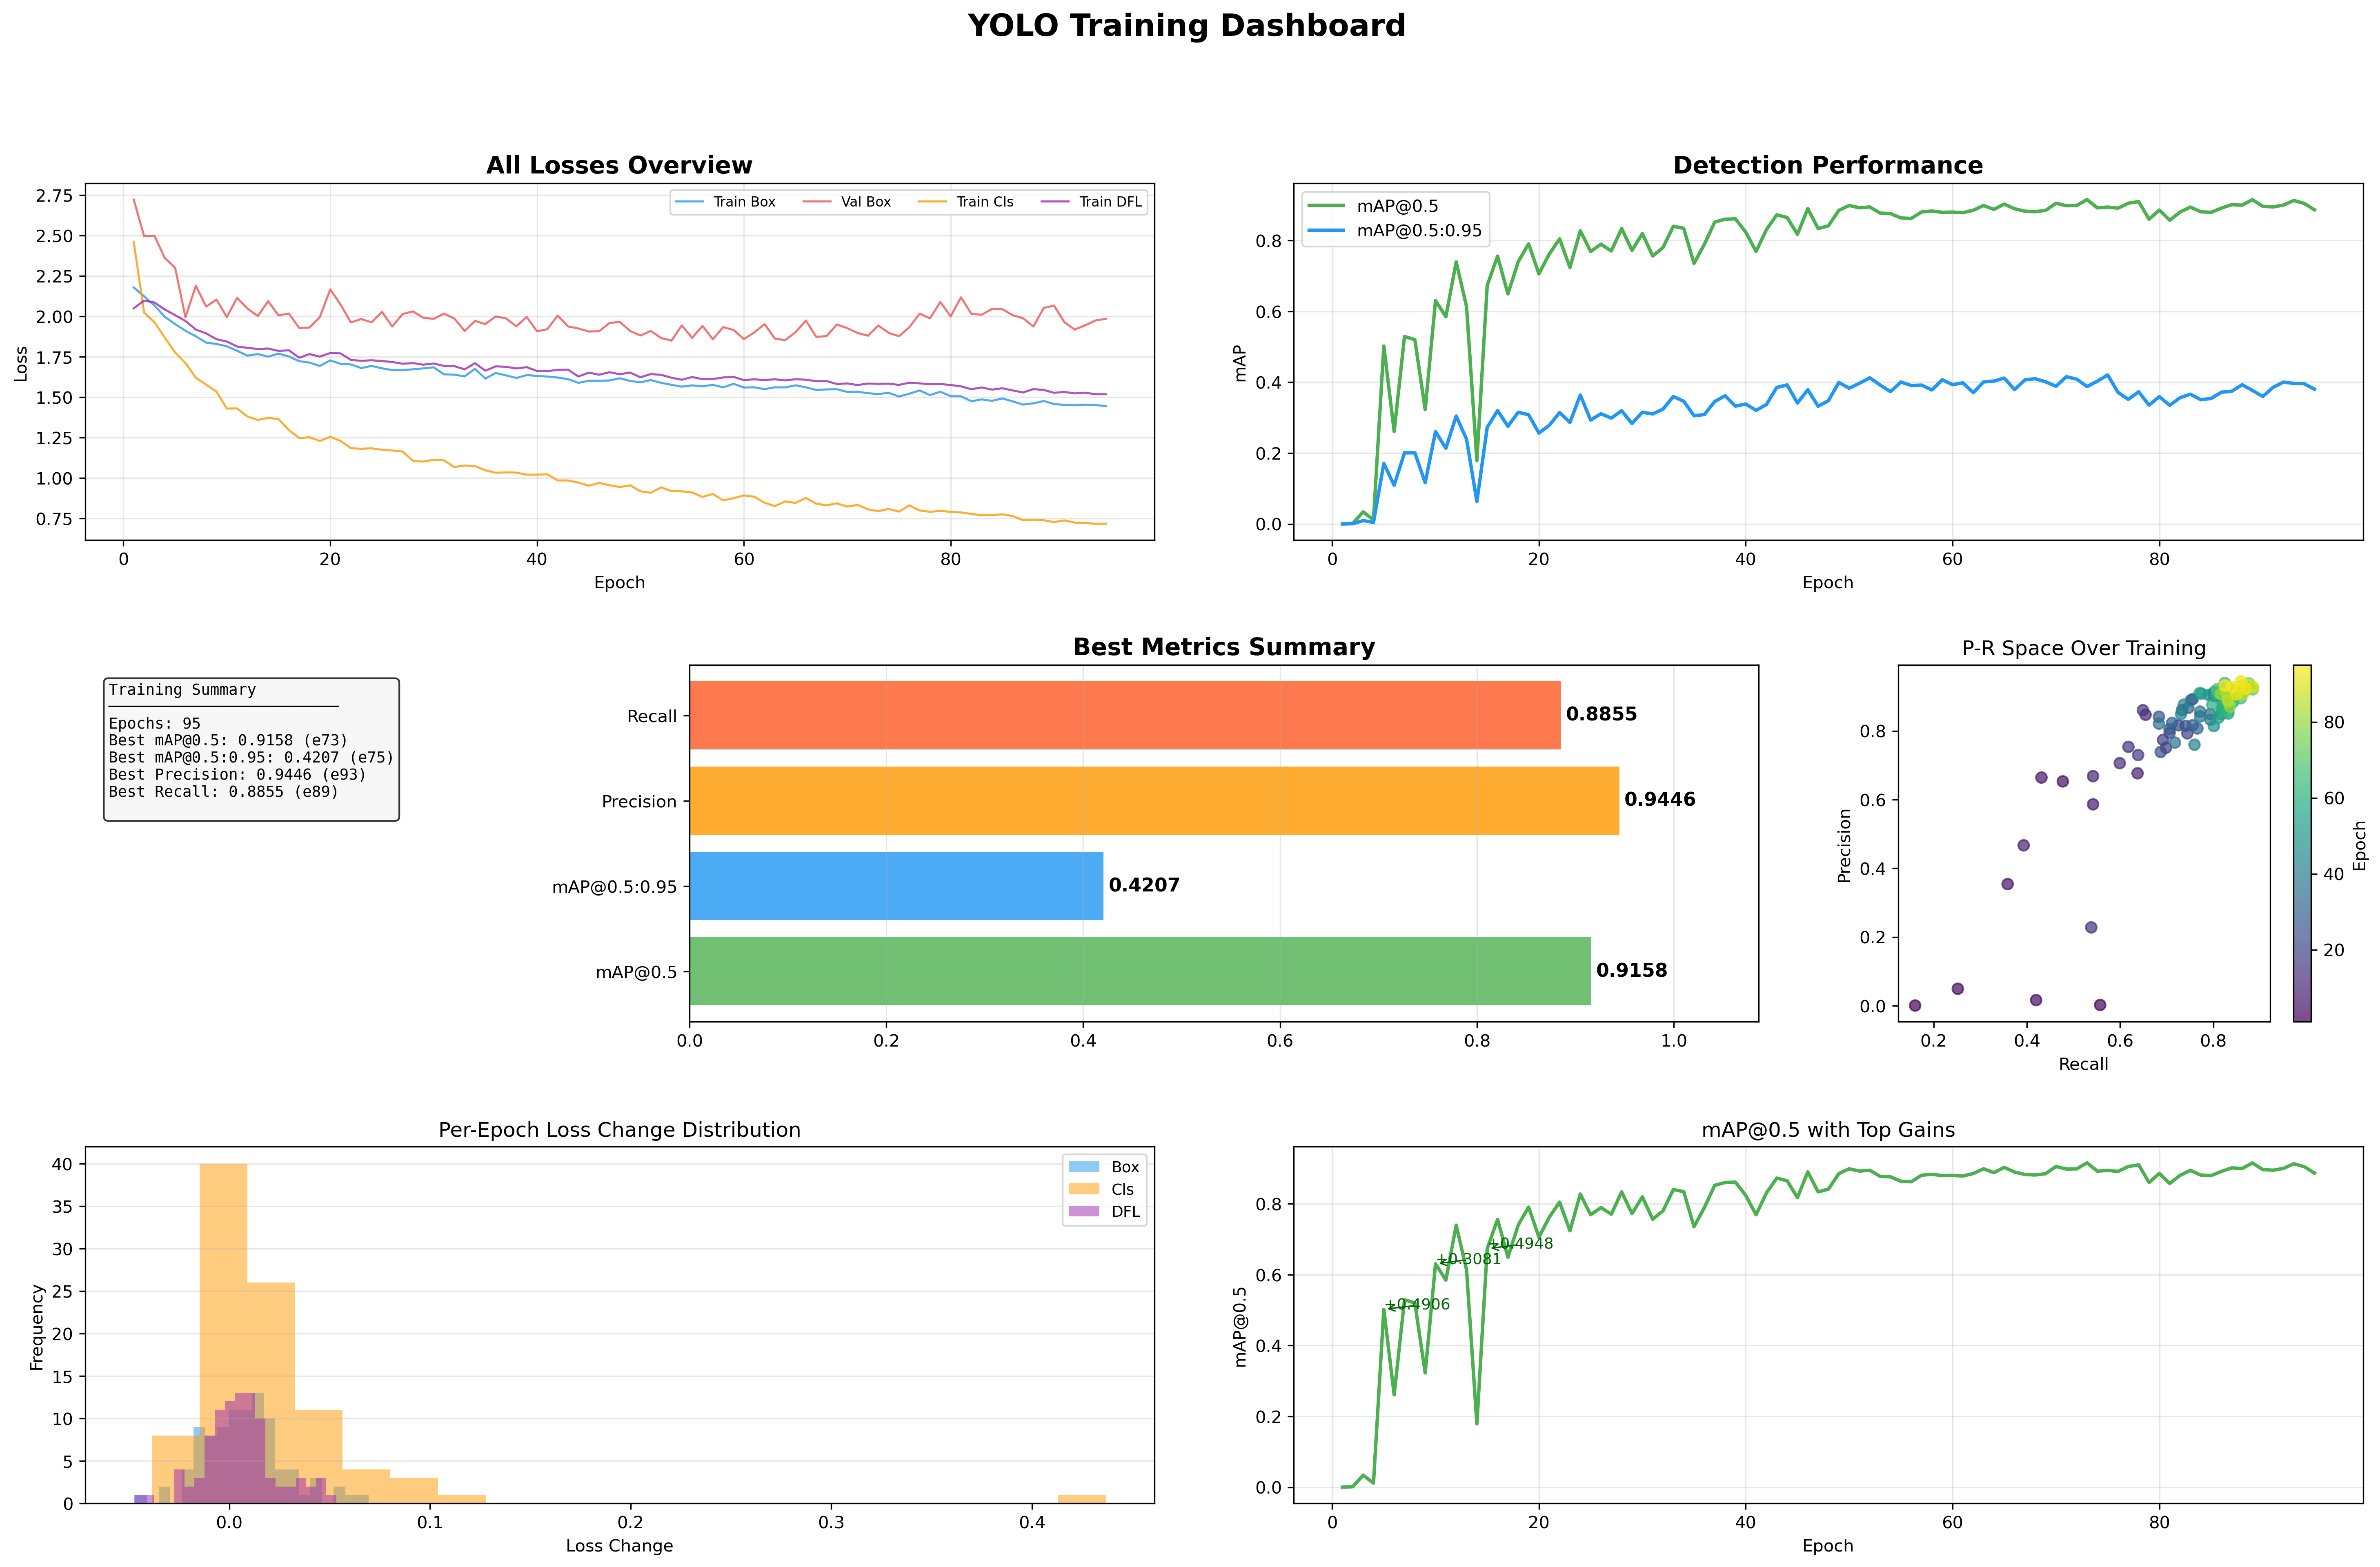
\includegraphics[width=0.92\linewidth]{figures/yolo/04_dashboard.png}
\caption{YOLO 训练过程综合仪表盘（损失、精度、召回率与 mAP）}
\label{fig:yolodash}
\end{figure}

第 95 轮（末轮）的验证指标为：精确率 0.928、召回率 0.840、mAP@0.5 为 0.905、mAP@0.5:0.95 为 0.396，全程最佳 mAP@0.5 达到 \textbf{0.916}。

从统计结果看，\textbf{精确率 0.928 与召回率 0.840 均较为优秀}：高精确率意味着报警结果可信、值班人员无需在大量误报中筛选，高召回率意味着绝大多数闯入目标都能被及时发现。两项指标同时保持在较高水平，说明模型在“不误报”与“不漏报”之间取得了良好平衡，能够满足低空无人机监测的使用要求；配合双目三角测量与多目标跟踪后，系统可在连续视频中稳定输出三维轨迹。



\begin{figure}[H]
\centering
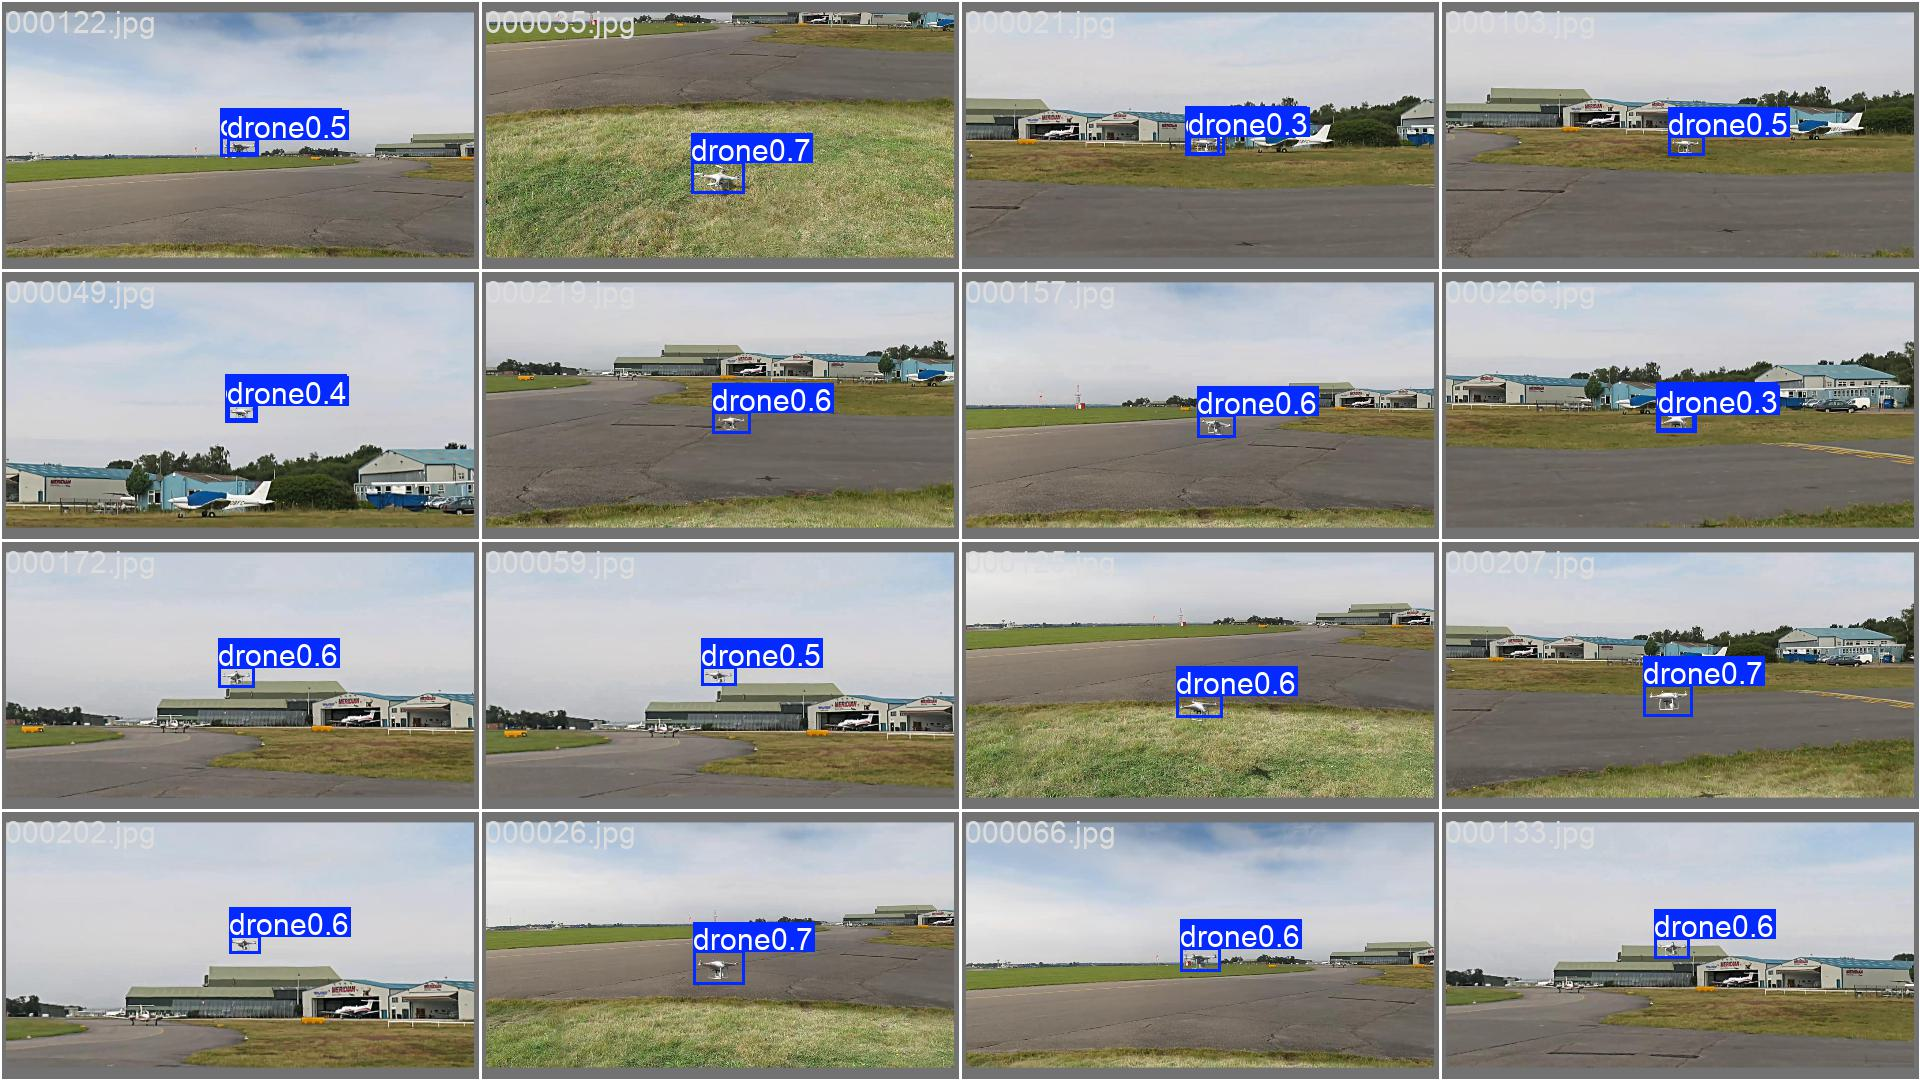
\includegraphics[width=0.78\linewidth]{figures/yolo/val_batch0_pred.jpg}
\caption{验证集检测结果示例（机场场景下的无人机目标）}
\label{fig:yolopred}
\end{figure}

从图~\ref{fig:yolopred} 可以看到，目标在画面中仅占数十像素，属于典型小目标检测场景；模型在草坪、跑道、机库等复杂背景下均能给出稳定框选，置信度集中在 0.3--0.7 之间，说明模型对该数据集的输出稳定、可信，与上述精确率与召回率的统计结果一致。

图~\ref{fig:yolopr} 给出验证集的 Precision--Recall 曲线：曲线整体靠近右上角，在不同置信度阈值下都能同时保持较高的精确率与召回率，说明模型对阈值选择不敏感，具备良好的部署适应性。

\begin{figure}[H]
\centering
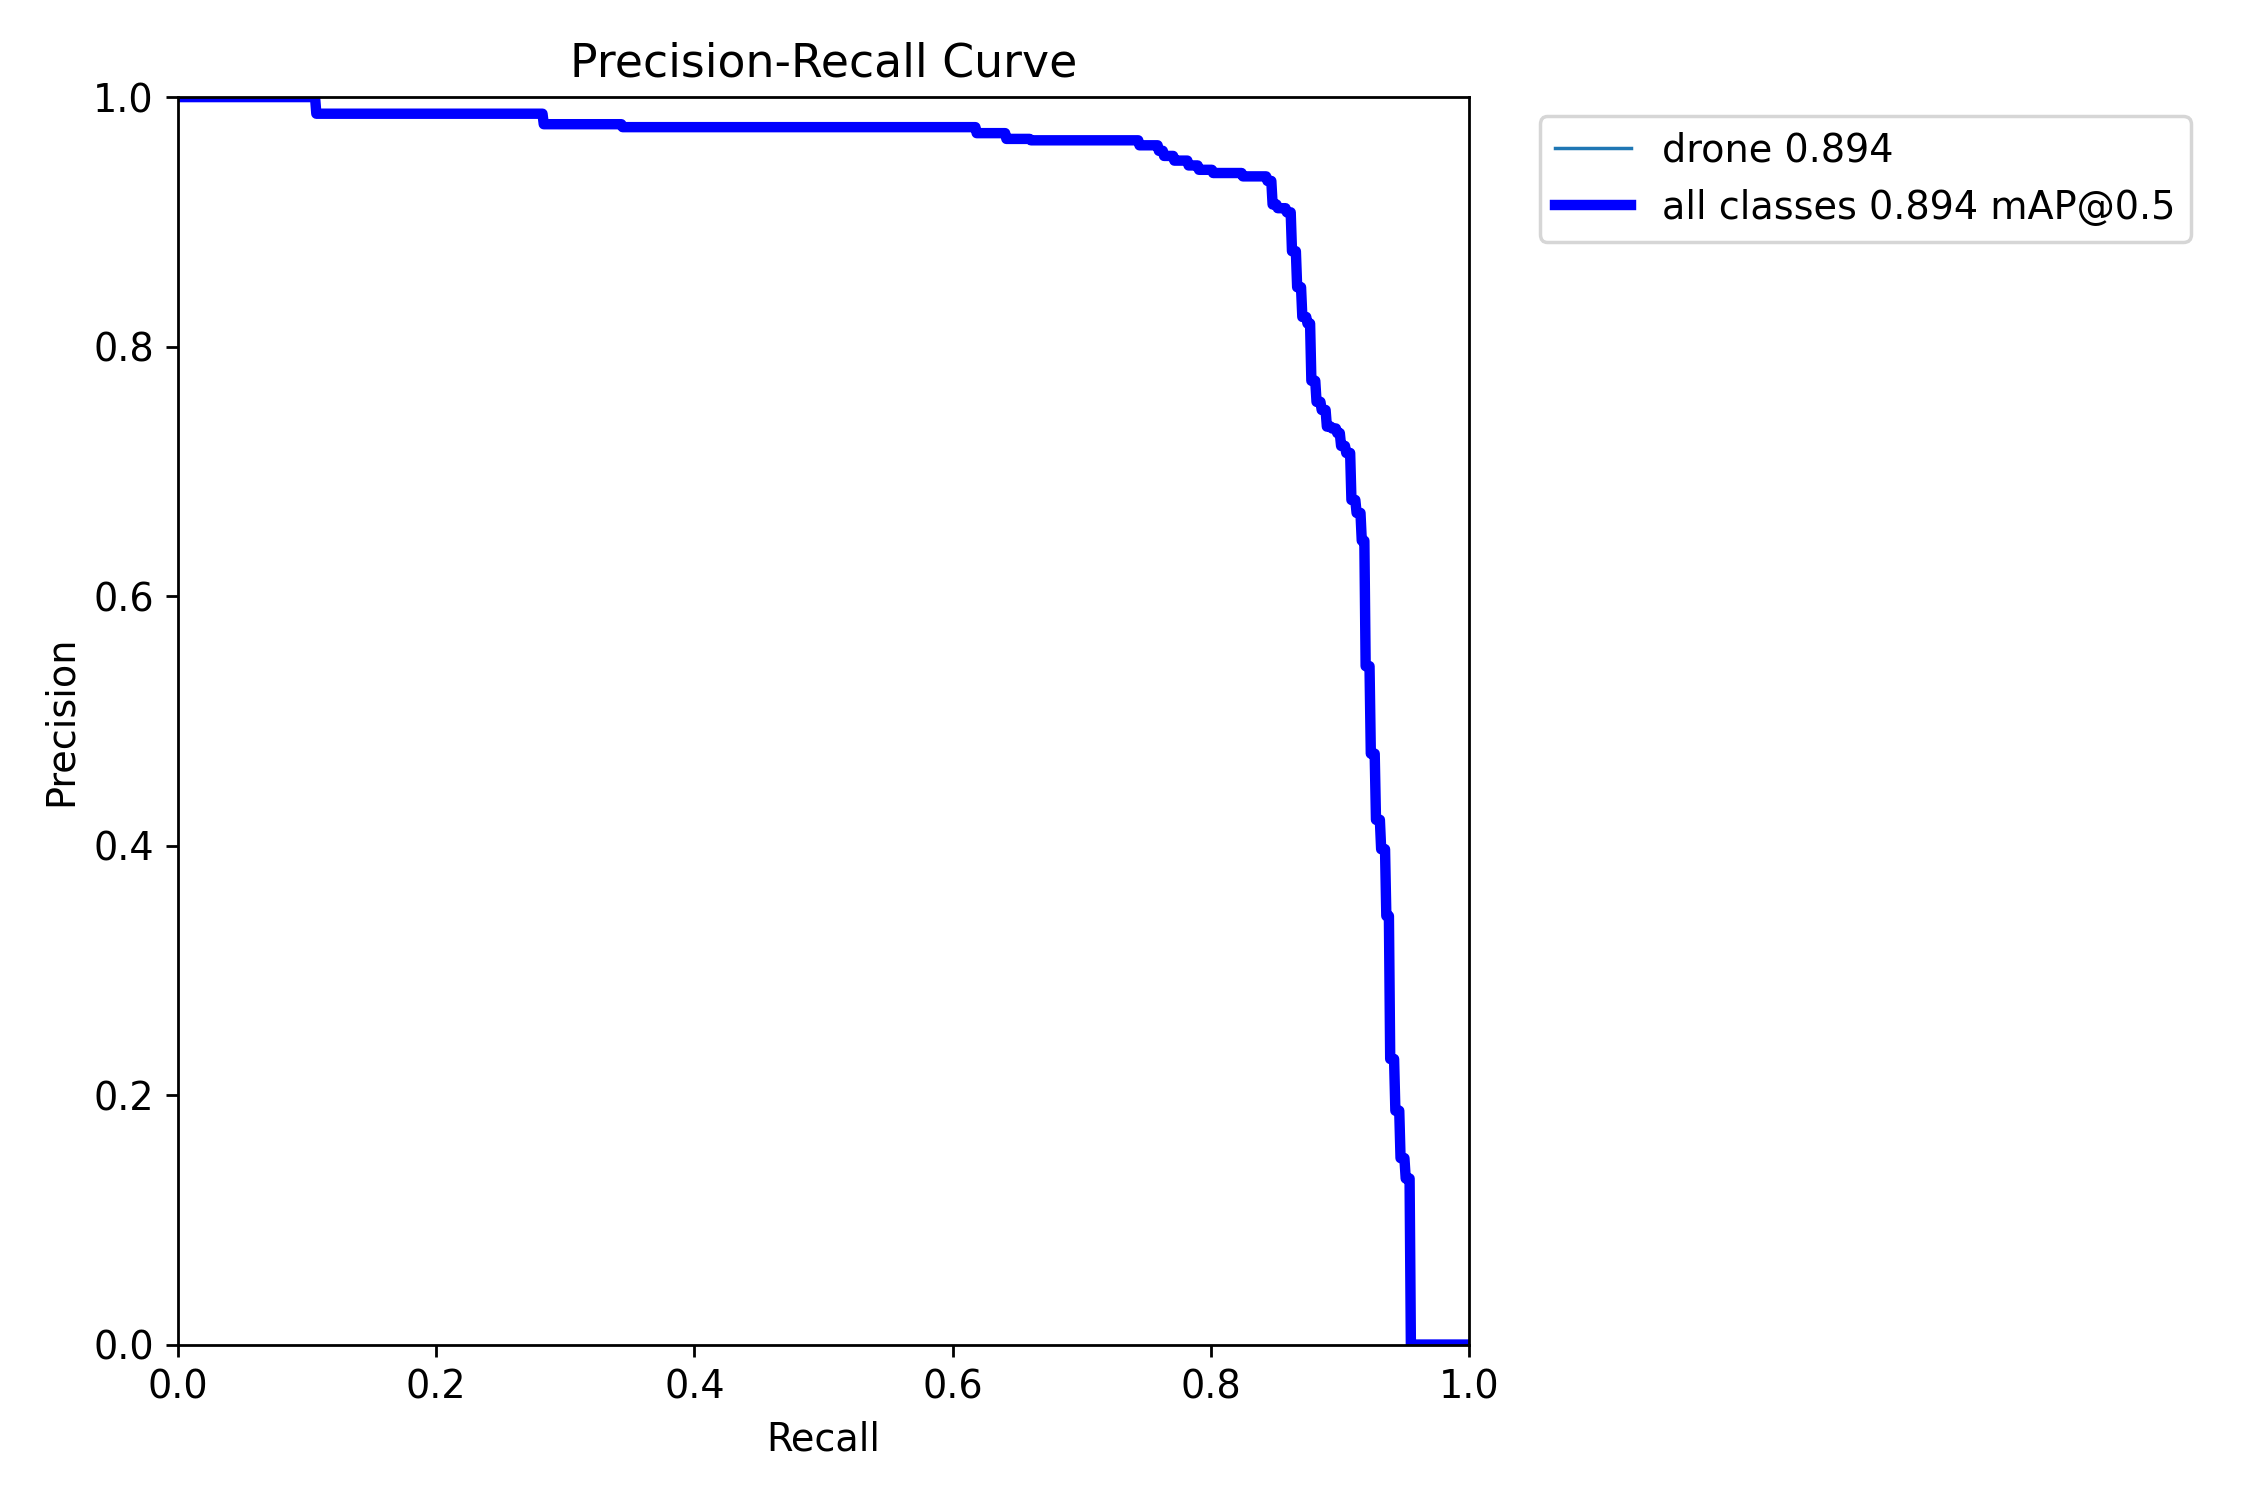
\includegraphics[width=0.78\linewidth]{figures/yolo/BoxPR_curve.png}
\caption{验证集 Precision--Recall 曲线}
\label{fig:yolopr}
\end{figure}

\subsection{多目标跟踪}

\code{MultiTracker} 支持两种工作模式，以适应不同的依赖条件：

\begin{enumerate}
  \item \term{ultralytics 内置跟踪}（推荐）：调用模型的跟踪接口并启用持久化与 ByteTrack 配置，由 ultralytics 完成 Kalman 预测与数据关联，直接返回稳定的跟踪 ID；\code{update_from_ultralytics()} 解析该结果并写入 \code{Track}。
  \item \term{独立 IOU 跟踪}（降级）：当内置跟踪不可用（未返回 ID 或未安装跟踪依赖）时，用贪心 IoU 匹配把当前帧检测关联到已有轨迹，IoU 低于阈值（默认 0.3）则新建轨迹。
\end{enumerate}

\code{Track} 对象同时保存 2D 与 3D 两条历史：\code{positions_2d}/\code{timestamps} 记录每帧的像素中心与时间，\code{positions}/\code{timestamps_3d} 只记录三角测量成功的点。两者分开保存的原因很关键：双目匹配并非每帧都成功，若把 3D 点按索引与 2D 时间戳对齐，会造成时间错位；因此 3D 点自带时间戳，写盘时以 \code{timestamps_3d} 为准。

轨迹的生命周期由三个参数控制：\code{max_missed_frames}（默认 30）决定连续多少帧未更新后判定丢失，\code{min_hits}（默认 3）决定累计命中多少次后才对外可见，从而抑制单帧误检产生的“幽灵轨迹”。

\subsection{双目三角测量}

\subsubsection{几何原理}

双目相机水平放置、光轴平行（或已知会聚角）时，同一目标在左右目图像上的横坐标差（视差）与深度成反比，如图~\ref{fig:stereo} 所示。

\begin{figure}[H]
\centering
\begin{tikzpicture}[x=1cm,y=1cm,font=\small]
% ---- 相机 ----
\draw[fill=cA, draw=cLine, rounded corners=1pt] (-0.45,-0.30) rectangle (0.45,0.30);
\draw[fill=cA, draw=cLine, rounded corners=1pt] (6.15,-0.30) rectangle (7.05,0.30);
\node[font=\scriptsize] at (0,0) {左目};
\node[font=\scriptsize] at (6.6,0) {右目};
% ---- 基线 ----
\draw[{Stealth[length=2mm]}-{Stealth[length=2mm]}, cLine] (0.45,-0.95) -- (6.15,-0.95);
\node[font=\scriptsize, fill=white, inner sep=1pt] at (3.3,-0.95) {基线 $B$};
% ---- 目标 ----
\coordinate (P) at (2.6,-4.5);
\node[circle, fill=cC, draw=cLine, inner sep=1.6pt] at (P) {};
\node[font=\scriptsize, anchor=west] at (2.78,-4.5) {目标 $P\;(x,y,z)$};
% ---- 视线 ----
\draw[cLine!70] (0,0.30) -- (P);
\draw[cLine!70] (6.6,0.30) -- (P);
% ---- 深度 ----
\draw[dashed, cLine] (2.6,-0.95) -- (2.6,-4.42);
\draw[{Stealth[length=2mm]}-{Stealth[length=2mm]}, cLine] (2.6,-1.15) -- (2.6,-4.28);
\node[font=\scriptsize, fill=white, inner sep=1pt, anchor=west] at (2.72,-2.9) {深度 $Z=\dfrac{f_xB}{d}$};
% ---- 直角标记 ----
\draw[cLine] (2.6,-1.15) -- (2.75,-1.15) -- (2.75,-1.30);
% ---- 说明 ----
\node[draw=cLine, dashed, rounded corners=2pt, fill=cD, align=left, font=\scriptsize, anchor=north west]
  at (-1.2,-5.55) {左、右目成像中目标的横坐标之差即视差 $d=x_l-x_r$，\\ 深度与视差成反比：视差越大，目标越近。};
\end{tikzpicture}
\caption{双目三角测量几何关系}
\label{fig:stereo}
\end{figure}

\subsubsection{焦距与主点}

若配置给出了像素焦距则直接使用；否则由视场角与分辨率推算：
\begin{equation}
f_x=\frac{W}{2\tan\left(\mathrm{FOV}_h/2\right)},\qquad
f_y=\frac{H}{2\tan\left(\mathrm{FOV}_v/2\right)}
\end{equation}
主点取图像中心 $(c_x,c_y)=(W/2,\,H/2)$，这是“无畸变标定信息时的合理假设”，工程上可通过标定文件替换。

\subsubsection{三角测量公式}

对左右目匹配框的中心点 $(x_l,y_l)$、$(x_r,y_r)$，视差 $d=x_l-x_r$，则
\begin{equation}
Z=\frac{f_x B}{d}
\end{equation}
\begin{equation}
X=\frac{(x_l-c_x)\,Z}{f_x}-\frac{B}{2},\qquad
Y=\frac{\left(\dfrac{y_l+y_r}{2}-c_y\right)Z}{f_y}
\end{equation}
其中 $B$ 为基线距离。$Y$ 取左右目纵坐标均值，可减小未完全行对齐带来的误差。输出坐标系为 OpenCV 相机系：$X$ 向右、$Y$ 向下、$Z$ 向前，原点位于双目光心中点。

\subsubsection{有效性校验}

三角测量前有三道校验：视差必须至少 1 像素且不小于由最大深度反推的下限；解算深度须落在 $[0.5\,\mathrm{m},\,2000\,\mathrm{m}]$；若深度超过由最小视差反推的上限，同样判为无效。任一校验失败返回 \code{None}，由调用方跳过该目标，绝不产生“无穷远”的异常点。

\subsection{跨目匹配}

左右目检测结果需要正确配对才能测距。\code{match_detections()} 采用“约束过滤 + 综合评分 + 贪心选择”的三段式策略。

\begin{enumerate}
  \item \term{硬约束}（不满足直接排除）：类别一致；垂直偏差 $|y_l-y_r|<50$ px；视差为正且在 $[d_{\min},d_{\max}]$ 内；左右框面积比不超过 2.0。
  \item \term{评分}（越小越好）：
  \begin{equation}
  s=\underbrace{|y_l-y_r|}_{\text{对齐误差}}
   +\underbrace{20\cdot\frac{|d-d_{\text{exp}}|}{d_{\text{exp}}}}_{\text{视差偏离}}
   +\underbrace{50\,(r_A-1)}_{\text{尺寸偏差}}
  \end{equation}
  其中 $d_{\text{exp}}$ 为视差范围中值，$r_A=\max(A_l,A_r)/\min(A_l,A_r)$ 为面积比。
  \item \term{类别加权}：若配置了目标类别，命中类别的得分乘以 0.5，非目标类别乘以 2.0，使无人机优先于飞鸟、飞机被配对。
\end{enumerate}

每个左目目标独立挑选得分最低且未被占用的右目目标（贪心），时间复杂度 $O(n^2)$；在单帧目标数通常小于 20 的场景下开销可忽略。

\subsection{世界坐标变换}

三角测量得到的是相机系坐标，尚需转换到统一世界系（$X$ 右、$Y$ 上、$Z$ 前），才能与其它平台的数据融合。变换按“翻转 $\rightarrow$ 偏航 $\rightarrow$ 俯仰 $\rightarrow$ 横滚 $\rightarrow$ 平移”的顺序执行：

\begin{equation}
\begin{aligned}
&\text{翻转：} && y \leftarrow -y\\
&\text{偏航 } \psi\text{：} && x' = x\cos\psi + z\sin\psi,\quad z' = z\cos\psi - x\sin\psi\\
&\text{俯仰 } \theta\text{：} && y' = y\cos\theta + z\sin\theta,\quad z' = z\cos\theta - y\sin\theta\\
&\text{横滚 } \phi\text{：} && x'' = x\cos\phi + y\sin\phi,\quad y'' = -x\sin\phi + y\cos\phi\\
&\text{平移：} && p_w = p'' + (p_x,p_y,p_z)
\end{aligned}
\end{equation}

该顺序等价于外旋（extrinsic）欧拉角 $R=R_z(\phi)R_x(\theta)R_y(\psi)$，与航空惯导的“偏航—俯仰—横滚”习惯一致。横滚的正方向做了特殊处理：绕 $Z$ 轴的正向旋转会使 $Y$ 轴倒向 $-X$（即左滚），因此右滚取 $-R_z(\phi)$。

\begin{notebox}[坐标约定提示]
配置中的 \code{pos_x/pos_y/pos_z} 是平台在世界系中的位置（米），\code{pitch/yaw/roll} 是平台朝向（度）。若平台安装方向与默认不一致，只需修改这六个参数，无需改代码。
\end{notebox}

\subsection{检测会话与并发模型}

一次检测任务对应一个 \code{DetectionSession} 对象，其状态迁移已在第~\ref{fig:sessstate} 节给出。会话的并发模型如下：

\begin{itemize}
  \item 每个会话拥有独立的后台守护线程，线程函数为 \code{_run_detection_pipeline()}；
  \item 主线程（Flask 请求线程）只负责创建会话、置位/清除事件标志、读取进度与预览帧，不参与计算；
  \item 进度、帧号、目标数、3D 点数等字段由工作线程写入、请求线程读取，均为单值写入，无需加锁；
  \item 预览帧以 JPEG 字节串缓存，接口 \code{/api/detection/preview} 直接返回，避免每次请求都重新编码；
  \item 会话注册表 \code{_sessions} 与“当前活跃会话”由 \code{_sessions_lock} 保护，防止并发创建/删除。
\end{itemize}

流水线的每个循环都执行“停止检查 $\rightarrow$ 暂停等待 $\rightarrow$ 取帧 $\rightarrow$ 检测 $\rightarrow$ 跟踪 $\rightarrow$ 匹配 $\rightarrow$ 三角测量 $\rightarrow$ 变换 $\rightarrow$ 关联”的固定序列，逻辑集中、便于定位问题。异常被捕获后写入 \code{error_message}，会话进入 \code{error} 状态而不是静默退出。

\subsection{数据桥接与落盘}

\code{tracks_to_dat()} 负责把内存中的多条轨迹合并成一个文件：

\begin{enumerate}
  \item 遍历所有 \code{Track}，收集 $(t,x,y,z)$ 四元组，时间戳取 \code{timestamps_3d}；
  \item 若没有任何 3D 点（双目全程未匹配成功），退化为写入 2D 像素坐标并将高度置 0，保证“至少有数据可回放”；
  \item 按时间排序后保存为 \file{.npz}（\code{positions}+\code{timestamps}）；
  \item 写入前调用 \code{backup_existing_fact()} 备份将被覆盖的文件，备份目录名带平台中文名，便于用户辨识；
  \item 删除同名旧 \file{.dat} 文件，避免两种格式并存导致读取歧义；
  \item 调用 \code{notify_reconstruction()} 向 5000 端口发送刷新请求，失败则静默忽略。
\end{enumerate}

\subsection{前端界面}

检测模块包含三个页面：检测工作台（视频上传、预览、控制、实时信息）、检测设置（模型与参数）、检测历史（文件与备份列表）。页面脚本分为 \file{detection.js}（接口通信封装）、\file{recognition.js}（工作台控制器）、\file{settings.js}、\file{history.js} 四个模块，通信层与界面层分离，便于替换界面而不改动接口逻辑。

工作台采用“双路上传 + 双路预览”布局：左右目各一个拖拽区，支持文件、流地址与摄像头 ID 三种输入；预览区并排显示两路带检测框的画面，右侧面板实时刷新状态、进度、目标数、3D 点数与已用时。

% ============================================================
%  第七章  轨迹预测（后续开发）
% ============================================================
\section{轨迹预测：现状与后续开发方案}
\label{sec:prediction_future}

\begin{notebox}[V2.0 修订说明]
本章描述的是 V1.0 的 Phy-ODE-Diffusion 方案，\textbf{已不再使用}。V2.0 的预测内核为 KinFlow，
训练/推理/评估详见 \file{docs/kinflow_prediction_model.md} 与版本说明表~\ref{tab:revision}。
本章保留作为设计过程记录。
\end{notebox}

本章说明轨迹预测功能的当前状态、失败原因与后续开发方案。需要明确的是：\textbf{本版本（V1.0）的轨迹预测尚未达到可用精度}，界面上的预测点实际由“线性外推”兜底算法产生，基于深度学习的混合模型仅完成了代码框架、训练脚本与权重加载链路，属于后续开发内容。

\subsection{现状说明}

\subsubsection{已实现的部分}

系统中与预测相关的代码已具备完整骨架：

\begin{itemize}
  \item \file{core/prediction/prediction.py}：预测入口、模型权重查找与缓存、线性外推兜底；
  \item \file{core/prediction/hybrid/}：Phy-ODE-Diffusion 模型定义（Transformer 编码器、物理 ODE 模块、扩散解码器、DDIM 采样器）；
  \item \file{services/predict_service.py}：单平台/全平台预测编排、时间轴对齐、综合预测合成；
  \item \file{train/hybrid_predictor/}：数据集加载、四旋翼动力学合成数据生成器、三阶段训练脚本；
  \item \file{models/hybrid_predictor/}：若干训练产出的检查点文件。
\end{itemize}

\subsubsection{未解决的部分}

当前版本存在三个层面的问题，导致混合模型无法投入使用：

\begin{enumerate}
  \item \term{权重与模型结构不匹配}。加载检查点时出现状态字典缺键错误：
\begin{lstlisting}[style=sh, caption={混合模型加载失败的运行日志（节选）}]
[预测] 模型加载失败: Error(s) in loading state_dict for PhyODEDiffusion:
    Missing key(s): "diffusion.lambda_zmax",
                    "diffusion.scheduler.alphas_cumprod", ...
    ，回退到线性外推
\end{lstlisting}
  根因是扩散模块中的若干缓冲区（高度上限缩放系数、扩散调度器的累积乘积表）在保存检查点时未被持久化，重新实例化模型后这些缓冲区已由构造函数生成，但状态字典中缺少对应条目，\code{load_state_dict(strict=True)} 因此失败。

  \item \term{训练数据不足且分布单一}。现有训练集主要由 \code{generate_synthetic.py} 按四旋翼动力学模型合成，缺少真实飞行数据；合成数据的运动模式（悬停、匀速盘旋、爬升）覆盖面有限，模型学到的是“生成器的分布”而非真实空域的运动分布。

  \item \term{缺少可信的评估闭环}。由于前两项问题，模型尚未在统一的验证协议下与线性外推做过对比，ADE/FDE 等指标无从谈起；现有检查点文件名中的 \code{v0.0249} 等数值是训练损失，不是位移误差，不能作为精度依据。
\end{enumerate}

\subsubsection{当前的实际行为}

预测接口 \code{/api/predict} 与 \code{/api/predict_all} 始终返回可用结果：当混合模型不可用（权重缺失、结构不匹配、历史点少于 10 个、推理异常）时，自动退回线性外推。线性外推以最后两点的速度向量延拓：

\begin{equation}
p_{n+k}=p_n+v\,\Delta t\,k,\qquad v=\frac{p_n-p_{n-1}}{t_n-t_{n-1}}
\end{equation}

该算法计算量极小、结果稳定，但假设“速度恒定”，对转弯、加速、爬升等机动完全无能为力。图~\ref{fig:use_analysis} 中可见可见光平台的预测高度持续下降并跌至负值，正是线性外推无法感知“无人机不会穿过地面”这一物理约束的表现。

因此，本版本对预测功能的定位是“\textbf{占位与兜底}”：接口、页面、数据结构、时间轴对齐逻辑均已就绪，后续替换预测内核时无需改动上层代码。

\subsection{需求分析}

后续开发需满足以下指标，方可称为“可用”：

\begin{table}[H]
\centering
\caption{轨迹预测功能的验收指标}
\label{tab:predreq}
\small
\begin{tabularx}{\linewidth}{@{}>{\heiti}p{3.2cm}p{3.4cm}X@{}}
\toprule
指标 & 目标值 & 说明 \\
\midrule
ADE & $\leq 1.5$ m & 预测 10 步（约 3 秒）内的平均位移误差 \\
FDE & $\leq 3.0$ m & 末点位移误差 \\
物理违反率 & $\leq 2\%$ & 高度越界、速度/加速度超限的预测点占比 \\
推理时延 & $\leq 150$ ms（GPU）\newline $\leq 800$ ms（CPU） & 单平台 20 点预测，10 步 DDIM 采样 \\
可用性 & 100\% & 任何异常都必须回退到线性外推，接口不得失败 \\
\bottomrule
\end{tabularx}
\end{table}

\subsection{技术路线：Phy-ODE-Diffusion}

拟采用的模型把“数据驱动”与“物理约束”结合，整体结构如图~\ref{fig:hybridarch} 所示。

\begin{figure}[H]
\centering
\begin{tikzpicture}[x=1cm,y=1cm,
  blk/.style={draw=cLine, line width=0.5pt, fill=cA, rounded corners=2pt,
              minimum height=0.9cm, align=center, font=\scriptsize, inner sep=3pt}]
\node[blk, minimum width=2.9cm, fill=cB] (in)  at (0,0)     {历史轨迹\\$(t_i,p_i)_{i=1}^{N}$};
\node[blk, minimum width=3.2cm]          (enc) at (3.95,0)  {Transformer 编码器\\6 层 · 4 头};
\node[blk, minimum width=3.0cm, fill=cC] (ode) at (7.95,0)  {物理结构 ODE\\$\dot z=f_\theta(z,t)$};
\node[blk, minimum width=3.0cm]          (ctx) at (11.85,0) {上下文向量\\$c$};
\node[blk, minimum width=2.9cm, fill=cD] (phy) at (3.4,-2.3)  {物理约束\\速度 / 加速度 / 高度};
\node[blk, minimum width=3.4cm]          (dif) at (7.95,-2.3) {物理引导扩散\\$x_\tau\to x_0$};
\node[blk, minimum width=3.0cm, fill=cB] (out) at (11.85,-2.3){预测轨迹\\$\hat p_{n+1..n+K}$};
\draw[arr] (in) -- (enc);
\draw[arr] (enc) -- node[lbl, above]{$z_0$} (ode);
\draw[arr] (ode) -- node[lbl, above]{$c$} (ctx);
\draw[arr] (ctx.south) -| (dif.north);
\draw[arr] (phy) -- (dif);
\draw[arr] (dif) -- (out);
\end{tikzpicture}
\caption{Phy-ODE-Diffusion 混合预测模型结构（开发方案）}
\label{fig:hybridarch}
\end{figure}

\subsubsection{编码器}

Transformer 编码器把不等间隔的历史轨迹映射为隐状态序列。时间间隔通过时间嵌入（\code{dt_emb_dim}）注入，使模型能处理“采样率不恒定”的真实数据；位置编码与时间嵌入相加后进入自注意力层。

\subsubsection{物理结构 ODE}

隐状态在连续时间上演化，由神经常微分方程描述：
\begin{equation}
\frac{\mathrm{d}z(t)}{\mathrm{d}t}=f_\theta\big(z(t),\,t,\,c\big),\qquad z(t_0)=z_0
\end{equation}
其中 $f_\theta$ 为两层 MLP（隐藏维 128），$c$ 为编码器给出的上下文。用四阶 Runge--Kutta 积分求解，ODE 的“连续时间”特性使模型可以在任意时间点查询状态，天然适配变步长预测。

\subsubsection{物理引导扩散}

预测轨迹被视为一个待去噪的样本。前向扩散逐步加噪：
\begin{equation}
q(x_\tau\mid x_0)=\mathcal{N}\left(\sqrt{\bar\alpha_\tau}\,x_0,\;(1-\bar\alpha_\tau)\mathbf{I}\right)
\end{equation}
反向过程由网络预测噪声，并在每一步施加物理引导：
\begin{equation}
x_{\tau-1}=\mathrm{DDIM}\big(x_\tau,\;\epsilon_\theta(x_\tau,\tau,c)\big)
-\eta\,\nabla_{x}\mathcal{L}_{\text{phy}}(x)
\end{equation}
其中 $\mathcal{L}_{\text{phy}}$ 由四项组成：
\begin{equation}
\mathcal{L}_{\text{phy}}=\lambda_v\mathcal{L}_{\text{speed}}
+\lambda_a\mathcal{L}_{\text{accel}}
+\lambda_z\mathcal{L}_{\text{height}}
+\lambda_{\text{tilt}}\mathcal{L}_{\text{tilt}}
\end{equation}
分别惩罚速度超限、加速度超限、高度越界（$z_{\min}\leq z\leq z_{\max}$）与倾角超限（$a_h\leq g\tan\theta_{\max}$）。$\eta$ 为引导强度，可由配置项 \code{guidance_eta} 调整。

\subsubsection{三阶段训练}

\begin{enumerate}
  \item \term{阶段一：表征学习}。冻结扩散模块，以 MSE 训练编码器 + ODE + 读出层，学习“历史 $\rightarrow$ 未来”的确定性映射；
  \item \term{阶段二：扩散拟合}。冻结编码器与 ODE，训练扩散网络拟合残差分布，加入物理损失（权重 0.01）；
  \item \term{阶段三：联合微调}。解冻全部参数，以小学习率（$10^{-4}$）联合优化，采用 scheduled sampling 缓解 exposure bias。
\end{enumerate}

每阶段独立保存检查点，支持断点续训；warmup + 余弦退火的学习率策略用于稳定训练。

\subsection{已有基础与复用清单}

后续开发可直接复用以下成果，无需从零开始：

\begin{table}[H]
\centering
\caption{预测模块可复用的已有成果}
\label{tab:reuse}
\small
\begin{tabularx}{\linewidth}{@{}>{\raggedright\ttfamily\scriptsize}p{6.5cm}>{\raggedright\arraybackslash}X@{}}
\toprule
文件 / 组件 & 可复用内容 \\
\midrule
core/prediction/prediction.py & 权重查找优先级、设备回退、异常降级、缓存机制 \\
core/prediction/hybrid/model.py & 模型主体、前向接口 \code{predict()}、参数统计 \\
core/prediction/hybrid/diffusion.py & 前向/反向扩散、DDIM 采样、物理引导 \\
core/prediction/hybrid/physics\_ode.py & ODE 右端函数与 RK4 积分器 \\
core/prediction/hybrid/ode\_manager.py & 变步长积分与状态管理 \\
train/hybrid\_predictor/dataset.py & 滑动窗口采样、归一化、变长序列批处理 \\
train/hybrid\_predictor/generate\_synthetic.py & 四旋翼动力学合成数据（含噪声与丢帧） \\
train/hybrid\_predictor/train.py & 三阶段训练、检查点、指标计算与图表输出 \\
\bottomrule
\end{tabularx}
\end{table}

\subsection{待解决的关键问题}

\begin{table}[H]
\centering
\caption{后续开发需解决的关键问题}
\label{tab:issues}
\small
\begin{tabularx}{\linewidth}{@{}>{\heiti}p{3.0cm}>{\raggedright\arraybackslash}X@{}}
\toprule
问题 & 说明与对策 \\
\midrule
检查点兼容 & 缓冲区改为 \code{register_buffer(..., persistent=False)} 或加载时使用 \code{strict=False} 并显式校验关键参数；同时在保存时写入 \code{model_info}（层数、维度、约束参数）以便版本校验 \\
真实数据 & 采集不少于 200 条真实飞行轨迹（多机型、多天气、多背景），与合成数据按 1:1 混合训练，并做域随机化（噪声、丢帧、传输延迟） \\
评估协议 & 固定训练/验证/测试划分与随机种子，统一报告 MSE、ADE、FDE、物理违反率，并与线性外推、卡尔曼滤波、LSTM 基线对比 \\
长时预测 & 采用滚动预测 + 误差累积抑制（多步一致性损失），避免误差随步数指数增长 \\
推理性能 & 采用 DDIM 少步采样（10--20 步）、TorchScript 导出与 INT8 量化，控制在 200 ms 以内 \\
退化输出 & 增加输出合法性检查（高度、速度、加速度），越界即裁剪并记录，确保不出现“钻地”预测 \\
\bottomrule
\end{tabularx}
\end{table}

\subsection{开发计划}

后续开发按四个里程碑推进，计划如图~\ref{fig:gantt} 所示。

\begin{figure}[H]
\centering
\begin{tikzpicture}[x=1cm,y=1cm,font=\scriptsize]
% 时间轴（每月 1.55cm，共 6 个月）
\foreach \m in {0,1,...,6} {
  \draw[cLine!45] (\m*1.55,0.35) -- (\m*1.55,-4.05);
}
\foreach \m in {1,2,...,6} {
  \pgfmathsetmacro{\xc}{(\m-0.5)*1.55}
  \node[font=\scriptsize] at (\xc,0.62) {第 \m 月};
}
\draw[cLine] (0,0.35) -- (9.3,0.35);
% 任务名称（左侧）与条形
\node[anchor=east, font=\scriptsize] at (-0.35,-0.55) {M1 缺陷修复};
\node[anchor=east, font=\scriptsize] at (-0.35,-1.55) {M2 数据建设};
\node[anchor=east, font=\scriptsize] at (-0.35,-2.55) {M3 模型训练};
\node[anchor=east, font=\scriptsize] at (-0.35,-3.55) {M4 评估集成};
\fill[cA] (0,-0.30) rectangle (4.65,-0.80);
\fill[cB] (2.33,-1.30) rectangle (6.98,-1.80);
\fill[cC] (4.65,-2.30) rectangle (9.30,-2.80);
\fill[cD] (6.98,-3.30) rectangle (9.30,-3.80);
\draw[cLine!50] (0,-0.55) -- (4.65,-0.55);
\end{tikzpicture}
\caption{轨迹预测功能开发计划（示意）}
\label{fig:gantt}
\end{figure}

\begin{table}[H]
\centering
\caption{里程碑与交付物}
\label{tab:milestone}
\small
\begin{tabularx}{\linewidth}{@{}>{\heiti}p{1.4cm}>{\heiti}p{3.4cm}p{4.0cm}X@{}}
\toprule
编号 & 里程碑 & 交付物 & 验收标准 \\
\midrule
M1 & 缺陷修复 & 可正常加载的检查点、加载日志 & 状态字典无缺键，推理可跑通 \\
M2 & 数据建设 & 真实轨迹数据集、数据清洗脚本 & 不少于 200 条，覆盖 3 类机动 \\
M3 & 模型训练 & 三阶段训练权重、训练曲线 & 验证集 ADE $<2.0$ m \\
M4 & 评估集成 & 对比报告、集成后的服务 & ADE $\leq1.5$ m，时延 $\leq200$ ms \\
\bottomrule
\end{tabularx}
\end{table}

\subsection{与现有接口的兼容性}

后续实现不改变任何对外契约：

\begin{itemize}
  \item 函数签名 \code{generate_prediction(points, timestamps, num_points, time_step)} 与 \code{generate_prediction_hybrid(...)} 保持不变；
  \item 接口 \code{/api/predict} 的请求与响应字段保持不变；
  \item 配置项 \code{hybrid_model} 的键名不变，新增参数以“有默认值”的方式追加；
  \item 降级策略保留：新模型任何异常都必须回退到线性外推，保证界面永不报错。
\end{itemize}

因此，切换预测内核只需替换 \file{models/hybrid_predictor/} 下的权重并修正加载逻辑，前端与接口层无需任何改动。

% ============================================================
%  第八章  数据结构设计
% ============================================================
\section{数据结构设计}

系统的数据分为四类：轨迹数据（文件）、运行时状态（内存）、配置数据（JSON）与备份元数据（JSON）。本章逐一给出格式定义。

\subsection{轨迹数据文件}

\subsubsection{主格式 .npz}

轨迹以 NumPy 压缩归档保存，包含两个数组：

\begin{table}[H]
\centering
\caption{轨迹文件 .npz 的结构}
\label{tab:npz}
\small
\begin{tabularx}{\linewidth}{@{}>{\ttfamily}p{2.2cm}>{\ttfamily}p{2.4cm}>{\ttfamily}p{2.0cm}>{\raggedright\arraybackslash}X@{}}
\toprule
键名 & 形状 / 类型 & 单位 & 含义 \\
\midrule
positions & (N, 3) float32 & m & 三维坐标，列顺序为 $x$（右）、$y$（上）、$z$（前） \\
timestamps & (N,) float32 & s & 各点时间戳，单调不减 \\
\bottomrule
\end{tabularx}
\end{table}

读写由 \code{np.savez} / \code{np.load} 完成，文件扩展名统一为 \file{.npz}。选择该格式的理由是：二进制读写快、精度可控、可直接被训练脚本消费，且无需引入数据库。

\subsubsection{兼容格式 .dat}

纯文本，每行四个以空白分隔的浮点数：

\begin{lstlisting}[style=sh, caption={轨迹文本格式示例（data/fact/visible.dat）}]
12.3456 -3.2100 150.0000 0.0000
12.5120 -3.1850 150.1230 0.3000
12.6890 -3.1420 150.2450 0.6000
\end{lstlisting}

读取时忽略空行，字段不足四个的行被跳过；解析失败的行不会中断整个文件，仅被忽略并返回已解析的部分。该格式用于人工准备数据、外部脚本导出与旧数据迁移。

\subsubsection{格式优先级}

加载器对同一“基名”按 \file{.npz} $\rightarrow$ \file{.dat} 的顺序尝试；恢复备份时若发现同名 \file{.dat} 与 \file{.npz} 并存，会主动删除被遮蔽的 \file{.npz}，确保恢复内容生效。

\subsection{平台标识与文件映射}

系统使用固定的平台标识串联前后端、配置与文件。映射关系如表~\ref{tab:platform} 所示。

\begin{table}[H]
\centering
\caption{平台标识与文件映射}
\label{tab:platform}
\small
\begin{tabularx}{\linewidth}{@{}>{\ttfamily\scriptsize}p{1.9cm}>{\scriptsize}p{1.7cm}>{\raggedright\ttfamily\scriptsize}p{3.4cm}>{\raggedright\ttfamily\scriptsize}p{3.1cm}>{\raggedright\arraybackslash}X@{}}
\toprule
标识 & 中文名 & 事实数据文件 & 预测数据文件 & 说明 \\
\midrule
visible & 可见光 & visible.npz & predict\_visible.npz & 默认平台 \\
infrared & 红外 & infrared.npz & predict\_infrared.npz & 默认平台 \\
radar & 雷达 & radar.npz & predict\_radar.npz & 默认平台 \\
self & 自选 & self.npz & predict\_self.npz & 上传数据后动态出现 \\
synthetic & 综合 & 不落盘 & predict\_synthetic.npz & 融合结果，运行期生成 \\
\bottomrule
\end{tabularx}
\end{table}

\subsection{运行时状态结构}

\subsubsection{平台状态字典}

全局字典 \code{detection_methods} 的每一项结构如下：

\begin{lstlisting}[style=py, caption={平台状态字典的字段}]
{
  "name":       str,      # 显示名称，如 "可见光"
  "color":      str,      # 十六进制颜色，如 "#ff6b6b"
  "visible":    bool,     # 是否在界面显示
  "enabled":    bool,     # 是否参与合成与预测
  "weight":     float,    # 融合权重（synthetic 无此字段）
  "points":     [[x, y, z], ...],   # 三维坐标序列
  "timestamps": [t, ...],           # 与 points 等长的时间戳
}
\end{lstlisting}

\subsubsection{检测对象}

\begin{table}[H]
\centering
\caption{检测与跟踪相关的数据结构}
\label{tab:detstruct}
\small
\begin{tabularx}{\linewidth}{@{}>{\ttfamily\scriptsize}p{3.4cm}>{\scriptsize}p{1.1cm}>{\raggedright\arraybackslash}X@{}}
\toprule
字段 & 类型 & 含义 \\
\midrule
\multicolumn{3}{@{}l}{\heiti Detection（单帧检测结果）} \\
bbox & list & $[x_1,y_1,x_2,y_2]$ 像素坐标（左上、右下） \\
confidence & float & 置信度，$[0,1]$ \\
class\_id & int & 类别编号 \\
class\_name & str & 类别名称 \\
\midrule
\multicolumn{3}{@{}l}{\heiti Track（单目标轨迹）} \\
track\_id & int & 跟踪 ID \\
positions / timestamps\_3d & list & 三维点及其时间戳（一一对应） \\
positions\_2d / timestamps & list & 二维中心点及其时间戳 \\
bboxes / confidences & list & 逐帧检测框与置信度 \\
first\_seen / last\_seen & float & 首次与最近一次出现时间 \\
is\_active & bool & 是否活跃 \\
frames\_since\_update & int & 连续未更新帧数 \\
\bottomrule
\end{tabularx}
\end{table}

\subsubsection{会话结构}

\code{DetectionSession} 由“可序列化字段”与“运行时对象”两部分组成。前者通过 \code{to_dict()} 暴露给前端，后者仅在服务端使用：

\begin{table}[H]
\centering
\caption{检测会话的字段划分}
\label{tab:session}
\small
\begin{tabularx}{\linewidth}{@{}>{\heiti}p{2.4cm}>{\ttfamily}p{6.0cm}>{\raggedright\arraybackslash}X@{}}
\toprule
类别 & 字段 & 说明 \\
\midrule
可序列化 & session\_id, status, progress & 会话编号、状态、进度 \\
 & current\_frame\_a/b, total\_frames & 双路帧号与总帧数 \\
 & track\_count, points\_3d & 活跃目标数、三维点数 \\
 & platform\_id, source\_a/b & 目标平台与视频源 \\
 & started\_at, finished\_at, error\_message & 时间与错误信息 \\
\midrule
运行时 & \_detector, \_tracker, \_stereo & 检测器、跟踪器、三角测量器 \\
 & \_thread, \_pause\_event, \_stop\_event & 后台线程与控制事件 \\
 & \_frame\_a, \_frame\_b & 最新预览帧（JPEG 字节串） \\
\bottomrule
\end{tabularx}
\end{table}

\subsection{备份元数据}

每个快照目录下的 \file{manifest.json} 描述该快照的内容：

\begin{lstlisting}[style=json, caption={备份清单 manifest.json 示例}]
{
  "created": "2026-10-28 12:53:49",
  "label": "可见光+红外+雷达",
  "methods": {
    "visible":  {"name": "可见光", "color": "#ff6b6b", "point_count": 60},
    "infrared": {"name": "红外",   "color": "#4ecdc4", "point_count": 60},
    "radar":    {"name": "雷达",   "color": "#ffe66d", "point_count": 60}
  },
  "files": {
    "fact":    ["visible.npz", "infrared.npz", "radar.npz"],
    "predict": ["predict_visible.npz"],
    "memory":  ["visible.npz", "infrared.npz", "radar.npz"]
  }
}
\end{lstlisting}

检测模块的备份使用同一结构（见 \file{data_bridge.py}），只是 \code{predict} 为空，从而两个模块的备份列表可以互认。

\subsection{配置结构}

配置文件分为十个顶层节，结构与用途如表~\ref{tab:conftree} 所示。完整字段说明见附录~B。

\begin{table}[H]
\centering
\caption{配置文件的顶层结构}
\label{tab:conftree}
\small
\begin{tabularx}{\linewidth}{@{}>{\raggedright\ttfamily\scriptsize}p{4.2cm}>{\raggedright\scriptsize}p{4.6cm}>{\raggedright\arraybackslash}X@{}}
\toprule
节名 & 主要内容 & 使用方 \\
\midrule
ai & 接口地址、密钥、模型名 & AI 策略 \\
detection\_methods & 五个平台的名称、颜色、权重、可见性 & 全部页面 \\
prediction\_settings & 预测点数上下限、默认点数、步长 & 预测页 \\
capture\_weights & 捕捉评分四项权重 & 分析页 \\
hybrid\_model & 混合模型开关、物理约束、设备 & 预测服务 \\
drone\_dynamics & 四旋翼动力学参数 & 训练与物理约束 \\
training & 训练超参（层数、维度、学习率、轮数） & 训练脚本 \\
detection & YOLO 模型路径、阈值、跟踪器、输入尺寸 & 检测服务 \\
platforms & 各平台双目内参、外参与位姿 & 检测服务 \\
theme / camera\_speed & 界面默认主题、相机移动速度 & 前端 \\
\bottomrule
\end{tabularx}
\end{table}

\subsection{报告文件}

AI 策略生成的报告以 Markdown 保存，文件名由 \code{strategy_} 前缀与 14 位时间戳组成，扩展名为 \code{.md}。内容包含：生成时间、参与平台列表、策略正文（由大模型返回）。报告保存在 \file{reports/} 目录，不参与数据融合，仅供查阅与归档。

% ============================================================
%  第九章  接口设计
% ============================================================
\section{接口设计}

系统对外提供四类接口：命令行接口、页面路由、REST 接口与前端脚本接口；此外还依赖一个外部 AI 接口。所有 REST 接口遵循统一约定：成功返回 \code{\{"success": true, ...\}}，失败返回 \code{\{"success": false, "error": "..."\}}，并配合适当的 HTTP 状态码。

\subsection{命令行接口}

\subsubsection{系统启动}

\begin{table}[H]
\centering
\caption{main.py 命令行参数}
\label{tab:cli}
\small
\begin{tabularx}{\linewidth}{@{}>{\raggedright\ttfamily\scriptsize}p{5.4cm}>{\raggedright\arraybackslash}X@{}}
\toprule
命令 & 说明 \\
\midrule
python main.py & 同时启动两个模块，并以桌面窗口打开重建模块 \\
python main.py --headless & 纯 HTTP 模式，不创建桌面窗口 \\
python main.py recon & 仅启动轨迹重建与分析（5000） \\
python main.py recog & 仅启动无人机检测（5001） \\
python -m trajectory\_reconstruction & 以模块方式启动重建分析 \\
python -m trajectory\_recognition & 以模块方式启动检测 \\
\bottomrule
\end{tabularx}
\end{table}

无论采用哪种方式，启动前都会扫描并终止占用 5000/5001 端口的残留进程，避免“端口被占用”导致的启动失败。

\subsubsection{训练脚本}

\begin{table}[H]
\centering
\caption{训练脚本参数}
\label{tab:traincli}
\small
\begin{tabularx}{\linewidth}{@{}>{\raggedright\ttfamily\scriptsize}p{4.5cm}>{\raggedright\ttfamily\scriptsize}p{3.0cm}>{\raggedright\arraybackslash}X@{}}
\toprule
脚本 & 常用参数 & 说明 \\
\midrule
train/yolotrain/train.py & --data / --model & 数据集描述文件与基础权重 \\
 & --epochs / --imgsz & 训练轮数与输入尺寸 \\
 & --batch / --device & 批次大小与设备（auto/cpu/cuda:0） \\
 & --freeze / --lr & 冻结层数与初始学习率 \\
 & --export / --format & 导出模型（onnx/engine/tflite） \\
 & --val & 仅验证，不训练 \\
\midrule
train/hybrid\_predictor/train.py & --stage & 训练阶段（1/2/3/all） \\
 & --epochs-s1..s3 & 各阶段轮数 \\
 & --batch-s1..s3 & 各阶段批次大小 \\
 & --resume & 从检查点恢复 \\
\bottomrule
\end{tabularx}
\end{table}

\subsection{页面路由}

\begin{table}[H]
\centering
\caption{页面路由}
\label{tab:pages}
\small
\begin{tabularx}{\linewidth}{@{}>{\ttfamily}p{3.0cm}>{\ttfamily}p{1.6cm}p{3.4cm}>{\raggedright\arraybackslash}X@{}}
\toprule
路径 & 模块 & 模板 & 页面说明 \\
\midrule
/ & 5000 & index.html & 总览：全屏三维轨迹视图 \\
/predict & 5000 & predict.html & 预测：参数设置与预测预览 \\
/analysis/ & 5000 & analysis.html & 分析：四联图与捕捉时机 \\
/ai & 5000 & ai.html & AI 策略：平台勾选与策略正文 \\
/data & 5000 & data.html & 数据：上传、备份、恢复 \\
/docs & 5000 & docs.html & 帮助文档中心 \\
/settings & 5000 & settings.html & 设置：主题、权重、模型参数 \\
/ & 5001 & index.html & 检测工作台 \\
/settings & 5001 & settings.html & 检测参数配置 \\
/history & 5001 & history.html & 检测历史与备份 \\
\bottomrule
\end{tabularx}
\end{table}

\subsection{REST 接口：轨迹重建与分析}

共 18 个接口，按功能分为四组，如表~\ref{tab:apirecon} 所示。

\begin{longtable}{@{}>{\ttfamily\scriptsize}p{1.3cm}>{\raggedright\ttfamily\scriptsize}p{4.2cm}>{\raggedright\ttfamily\scriptsize}p{3.4cm}>{\raggedright\arraybackslash}p{4.9cm}@{}}
\caption{轨迹重建与分析的 REST 接口}\label{tab:apirecon}\\
\toprule
{\heiti 方法} & {\heiti 路径} & {\heiti 请求参数} & {\heiti 返回} \\
\midrule
\endfirsthead
\multicolumn{4}{@{}l}{\small 续表~\thetable}\\
\toprule
{\heiti 方法} & {\heiti 路径} & {\heiti 请求参数} & {\heiti 返回} \\
\midrule
\endhead
\bottomrule
\endlastfoot
POST & /api/predict & method\_id, num\_points, time\_step & prediction, pred\_times \\
POST & /api/predict\_all & num\_points, time\_step & results\{平台: 预测\} \\
POST & /api/ai\_suggestion & methods\_data & suggestion \\
POST & /api/save\_report & content, platforms & filepath \\
POST & /api/refresh\_data & --- & success \\
POST & /api/load\_data & form: file, method\_id & success, name \\
POST & /api/clear\_all\_data & --- & backup\_name \\
POST & /api/toggle\_method & method\_id & visible \\
POST & /api/synthesize & --- & point\_count, platforms, weights \\
POST & /api/weights & synth\_weights 等 & success \\
POST & /api/hybrid\_model & v\_max, a\_max 等 & hybrid\_model \\
GET/POST & /api/theme & theme & theme \\
GET & /api/list\_backups & --- & backups[] \\
POST & /api/restore\_backup & backup\_file, full & message \\
POST & /api/restore\_all\_backups & --- & restored[] \\
POST & /api/backup/create & --- & name \\
POST & /api/backup/delete & backup\_name & message \\
GET & /analysis/data & --- & 各平台运动学序列 \\
GET & /analysis/capture & --- & 前三名捕捉时机 \\
\end{longtable}
其中 \code{/analysis/data} 与 \code{/analysis/capture} 挂在 \code{/analysis} 前缀下，其余接口未设前缀。

\subsection{REST 接口：无人机检测}

检测接口统一挂在 \code{/api/detection} 前缀下，共 12 个，如表~\ref{tab:apidet} 所示。

\begin{table}[H]
\centering
\caption{无人机检测的 REST 接口}
\label{tab:apidet}
\footnotesize
\begin{tabularx}{\linewidth}{@{}>{\ttfamily\scriptsize}p{1.2cm}>{\raggedright\ttfamily\scriptsize}p{3.3cm}>{\raggedright\ttfamily\scriptsize}p{3.9cm}>{\raggedright\arraybackslash}X@{}}
\toprule
方法 & 路径 & 参数 & 说明 \\
\midrule
POST & /start & 表单: video\_a, video\_b, config & 上传双路视频并启动会话 \\
POST & /stop & session\_id? & 停止检测 \\
POST & /pause & session\_id? & 暂停 \\
POST & /resume & session\_id? & 恢复 \\
GET & /status & session\_id? & 会话状态与进度 \\
GET & /tracks & session\_id?, format & 跟踪结果（summary/full） \\
GET & /preview & channel=a|b & 最新预览帧 JPEG \\
GET & /sessions & status? & 历史会话列表 \\
DELETE & /sessions/\{id\} & --- & 删除会话 \\
GET/POST & /config & detection/platforms & 读写检测配置 \\
GET & /models & --- & 可用模型列表 \\
GET & /files & --- & 轨迹文件列表 \\
DELETE & /files/\{name\} & --- & 删除轨迹文件 \\
GET & /backups & --- & 备份列表 \\
POST & /save & session\_id?, platform\_id & 保存轨迹到 data/fact \\
\bottomrule
\end{tabularx}
\end{table}

\subsection{前端脚本接口}

页面脚本通过 \code{window._PAGE_DATA_} 获取服务端注入的数据，通过 \code{fetch} 调用上述接口。检测模块把通信封装为 \code{DetectionAPI} 对象，主要方法如表~\ref{tab:jsapi} 所示。

\begin{table}[H]
\centering
\caption{前端脚本的主要接口}
\label{tab:jsapi}
\small
\begin{tabularx}{\linewidth}{@{}>{\raggedright\ttfamily\scriptsize}p{5.4cm}>{\raggedright\arraybackslash}X@{}}
\toprule
方法 / 对象 & 说明 \\
\midrule
DetectionAPI.start(formData) & 提交双路视频与配置，返回会话信息 \\
DetectionAPI.status(sessionId) & 轮询状态、进度与统计 \\
DetectionAPI.previewUrl(channel) & 生成预览图 URL \\
DetectionAPI.tracks(sessionId) & 拉取跟踪摘要 \\
DetectionAPI.save(payload) & 保存轨迹到共享目录 \\
toast.show/error/success & 统一的通知浮层 \\
buildAxes / buildLights & 构建三维坐标轴与光照 \\
bindWASD / bindCoordTooltip & 键盘漫游与坐标拾取 \\
\bottomrule
\end{tabularx}
\end{table}

\subsection{外部 AI 接口}

AI 策略调用遵循 OpenAI Chat Completions 协议：

\begin{lstlisting}[style=json, basicstyle=\ttfamily\scriptsize, caption={AI 策略的请求体结构}]
{
  "model": "Qwen/Qwen2.5-7B-Instruct",
  "messages": [
    {"role": "system", "content": "无人机反制专家……"},
    {"role": "user", "content": "检测手段: 可见光 ……”}
  ],
  "temperature": 0.7,
  "max_tokens": 800
}
\end{lstlisting}

响应取 \code{choices} 数组首项的 \code{message.content}。系统对四类异常分别给出可读提示：请求超时、HTTP 错误、响应非 JSON、响应缺少 \code{choices} 字段。

\subsection{响应约定与错误处理}

\begin{table}[H]
\centering
\caption{HTTP 状态码与响应约定}
\label{tab:http}
\small
\begin{tabularx}{\linewidth}{@{}>{\heiti}p{1.6cm}>{\ttfamily}p{4.4cm}>{\raggedright\arraybackslash}X@{}}
\toprule
状态码 & 响应体 & 触发条件 \\
\midrule
200 & \{"success": true, ...\} & 请求成功 \\
400 & \{"success": false, "error"\} & 参数缺失、格式错误、数据不足 \\
404 & \{"success": false, "error"\} & 接口或资源不存在 \\
500 & \{"success": false, "error"\} & 服务内部异常（不暴露堆栈） \\
204 & 空响应 & 检测预览暂无可用帧 \\
\bottomrule
\end{tabularx}
\end{table}

所有响应统一添加禁止缓存的响应头（\code{Cache-Control: no-store}），确保前端始终加载最新脚本与数据。

% ============================================================
%  第十章  软件使用说明
% ============================================================
\section{软件使用说明}

本章说明软件“怎么用”。先介绍界面风格与通用操作，再按页面给出标注了编号的界面截图、操作步骤与区域用途说明，最后把常用操作串成三条典型流程，并汇总常见问题。截图取自 V1.0 实际运行界面（默认深色主题，1600$\times$1000 视口）。

\subsection{快速上手}

\subsubsection{启动与入口}

软件有两个入口（表~\ref{tab:use_entry}）。日常使用推荐第一种，双击或执行一条命令即可同时启动两个模块并打开桌面窗口。

\begin{table}[H]
\centering
\caption{启动方式与访问地址}
\label{tab:use_entry}
\small
\begin{tabularx}{\linewidth}{@{}>{\ttfamily}p{4.4cm}>{\raggedright\arraybackslash}X@{}}
\toprule
命令 & 说明 \\
\midrule
python main.py & 桌面窗口，两个模块同时运行（推荐） \\
python main.py --headless & 不弹窗口，用浏览器访问两个地址 \\
python main.py recon & 只启动轨迹重建与分析（5000） \\
python main.py recog & 只启动无人机检测（5001） \\
\bottomrule
\end{tabularx}
\end{table}

启动成功后，浏览器访问 \url{http://127.0.0.1:5000} 进入轨迹重建与分析，访问 \url{http://127.0.0.1:5001} 进入无人机检测；在 5000 页面点击导航栏右侧的“识别”可直接跳转到检测模块。

\subsubsection{首次使用要做的三件事}

\begin{enumerate}
  \item \term{准备数据}：\file{data/fact/} 目录下至少有一个平台的轨迹文件（如 \file{visible.npz}）。软件自带示例数据，首次启动即可看到轨迹。
  \item \term{准备检测模型}：\file{models/yolo/detect.pt} 为检测权重；未放置时检测页仍可打开，但无法开始检测。
  \item \term{配置 AI 密钥（可选）}：编辑 \file{config.json} 的 \code{ai} 段，填入可用的接口地址、密钥与模型名，才能使用“AI 策略”；不配置不影响其它功能。
\end{enumerate}

\subsection{界面总览与通用操作}

\subsubsection{界面风格}

界面采用统一的设计语言，由 \file{templates/frontend/static/css/main.css} 中的 CSS 变量驱动：

\begin{itemize}
  \item \term{导航栏}：固定在顶部，左侧为品牌与五个主功能入口，右侧为“识别 / 帮助 / 设置”三个辅助入口；当前页高亮。
  \item \term{面板}：半透明毛玻璃背景、1 px 描边、8 px 圆角；面板标题左侧配线性图标。
  \item \term{配色}：深色主题以深蓝灰为底，主色为蓝色，五个平台各有专属颜色（可见光珊瑚红、红外青绿、雷达黄、自选橙、综合白）。
  \item \term{图形语言}：全部图标为几何风格 SVG，不使用 emoji；数值统一使用等宽字体，便于对齐比较。
  \item \term{双主题}：深色/浅色主题通过 \code{data-theme} 属性切换，所有颜色由变量定义，切换时无需刷新页面。
\end{itemize}

\subsubsection{界面结构}

两个模块界面风格一致：顶部导航栏、中间内容区、右下角浮层提示。以总览页为例，界面由五个部分组成（图~\ref{fig:use_dashboard}）。

\begin{figure}[H]
\centering
\begin{tikzpicture}
\node[inner sep=0, anchor=south west] (im) at (0,0)
  {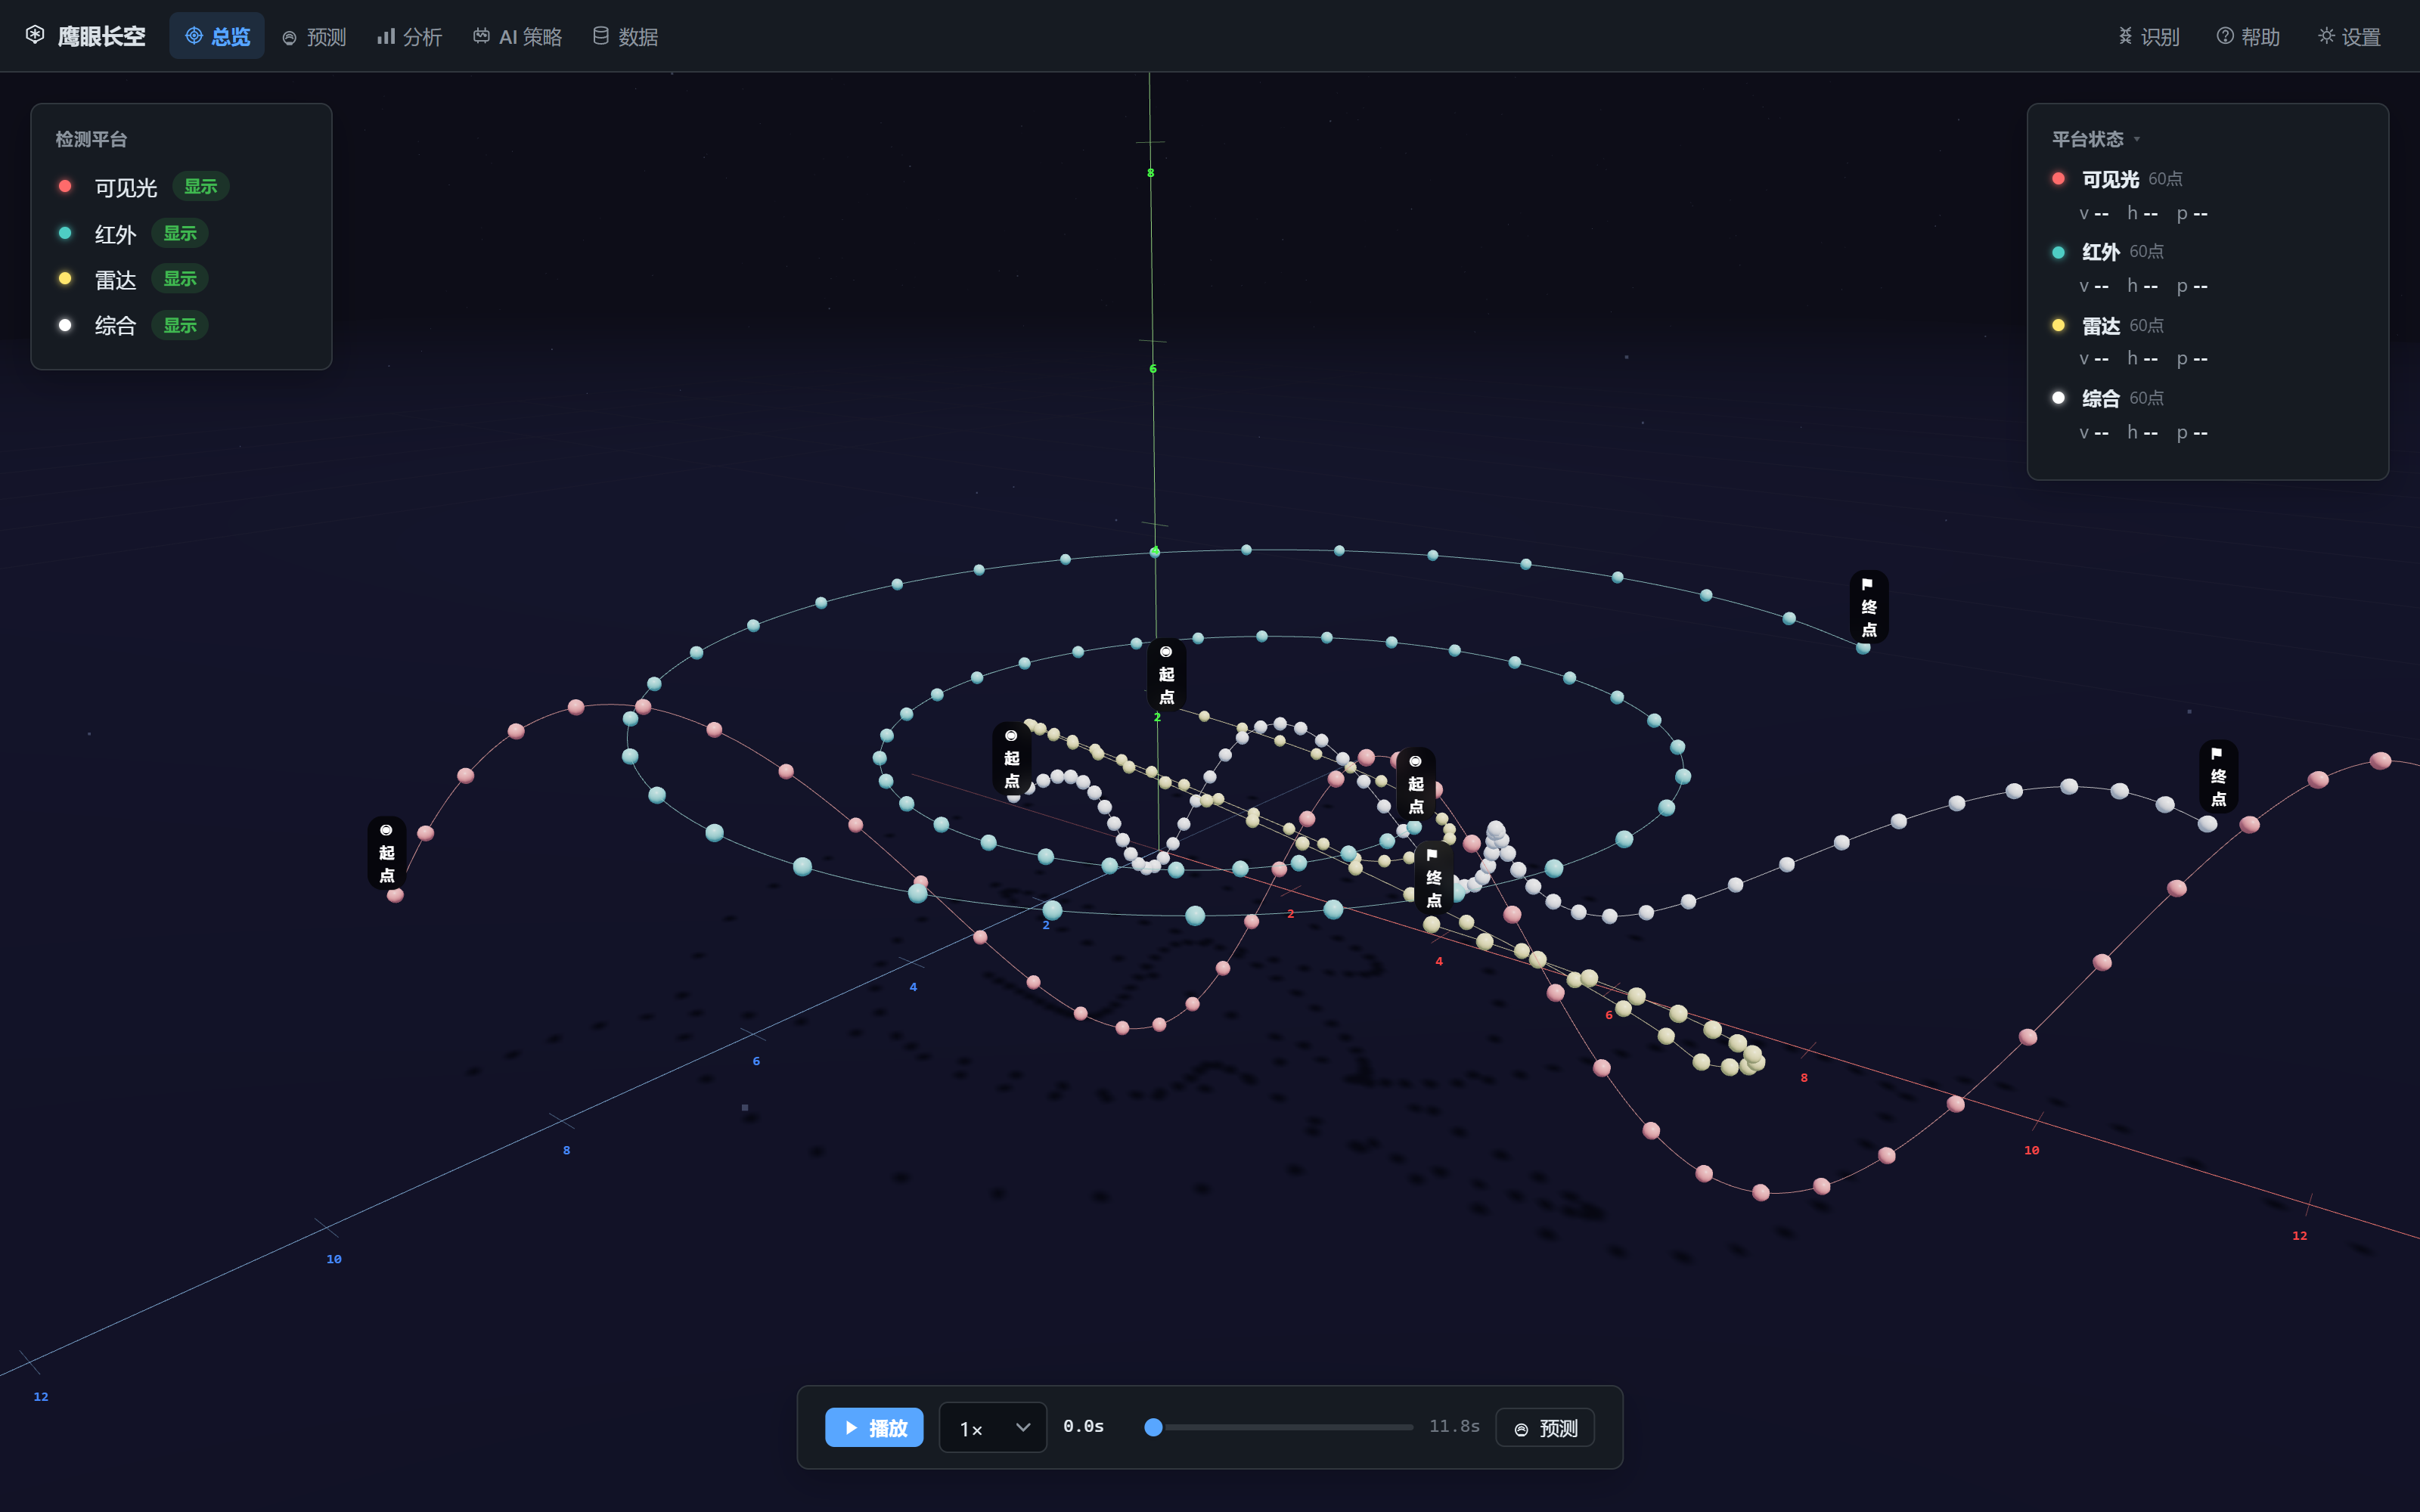
\includegraphics[width=\linewidth]{figures/ui/dashboard.png}};
\begin{scope}[x={(im.south east)},y={(im.north west)}]
  \hotspot{1}{0.115}{0.880}
  \hotspot{2}{0.945}{0.880}
  \hotspot{3}{0.500}{0.430}
  \hotspot{4}{0.345}{0.052}
  \hotspot{5}{0.640}{0.978}
\end{scope}
\end{tikzpicture}
\caption{总览页操作区域：\cn{1}~检测平台面板\quad \cn{2}~平台状态面板\quad \cn{3}~三维轨迹场景\quad \cn{4}~时间轴控制条\quad \cn{5}~顶部导航栏}
\label{fig:use_dashboard}
\end{figure}

\begin{enumerate}
  \item \term{检测平台面板（左上，\cn{1}）}：每一项左侧圆点为该平台颜色，右侧按钮切换“显示/隐藏”；隐藏只影响绘制，不删除数据。
  \item \term{平台状态面板（右上，\cn{2}）}：显示各平台点数与当前时刻的速度 $v$、高度 $h$、位置 $p$，随播放实时刷新；点击标题可折叠。
  \item \term{三维轨迹场景（\cn{3}）}：彩色曲线为各平台轨迹，白色为加权融合的综合轨迹；每条轨迹标注起点与终点，中央坐标轴标注 $X$（红）、$Y$（绿）、$Z$（蓝）。
  \item \term{时间轴控制条（\cn{4}）}：播放/暂停、倍速（0.5×--4×）、当前时刻、进度滑块与总时长；右侧“预测”按钮直达预测页。
  \item \term{顶部导航栏（\cn{5}）}：左侧五个主功能入口（总览、预测、分析、AI 策略、数据），右侧“识别 / 帮助 / 设置”；当前页面入口高亮。
\end{enumerate}

\subsubsection{三维视图操作}

\begin{table}[H]
\centering
\caption{三维视图与常用操作}
\label{tab:use_ops}
\small
\begin{tabularx}{\linewidth}{@{}>{\heiti}p{4.0cm}>{\raggedright\arraybackslash}X@{}}
\toprule
操作 & 效果 \\
\midrule
按住左键拖动 & 绕视点旋转，换角度观察轨迹 \\
滚动滚轮 & 拉近 / 拉远 \\
按住右键拖动 & 平移视点 \\
W / S / A / D & 相机前后左右移动 \\
Q / E & 相机下降 / 上升 \\
鼠标悬停轨迹点 & 球体放大并弹出该点坐标与时刻 \\
空格键 & 播放 / 暂停动画 \\
\bottomrule
\end{tabularx}
\end{table}

\begin{notebox}[两个实用技巧]
轨迹重叠时，先在左侧面板隐藏部分平台逐个观察；相机移动速度可在 \file{config.json} 的 \code{camera_speed} 中调整（默认 0.1）。所有操作结果以右下角浮层提示反馈：绿色成功、红色失败、黄色警告。
\end{notebox}

\subsection{轨迹重建与分析的操作}

\subsubsection{预测页}

预测页在历史轨迹之后叠加预测段（图~\ref{fig:use_predict}）。

\begin{figure}[H]
\centering
\begin{tikzpicture}
\node[inner sep=0, anchor=south west] (im) at (0,0)
  {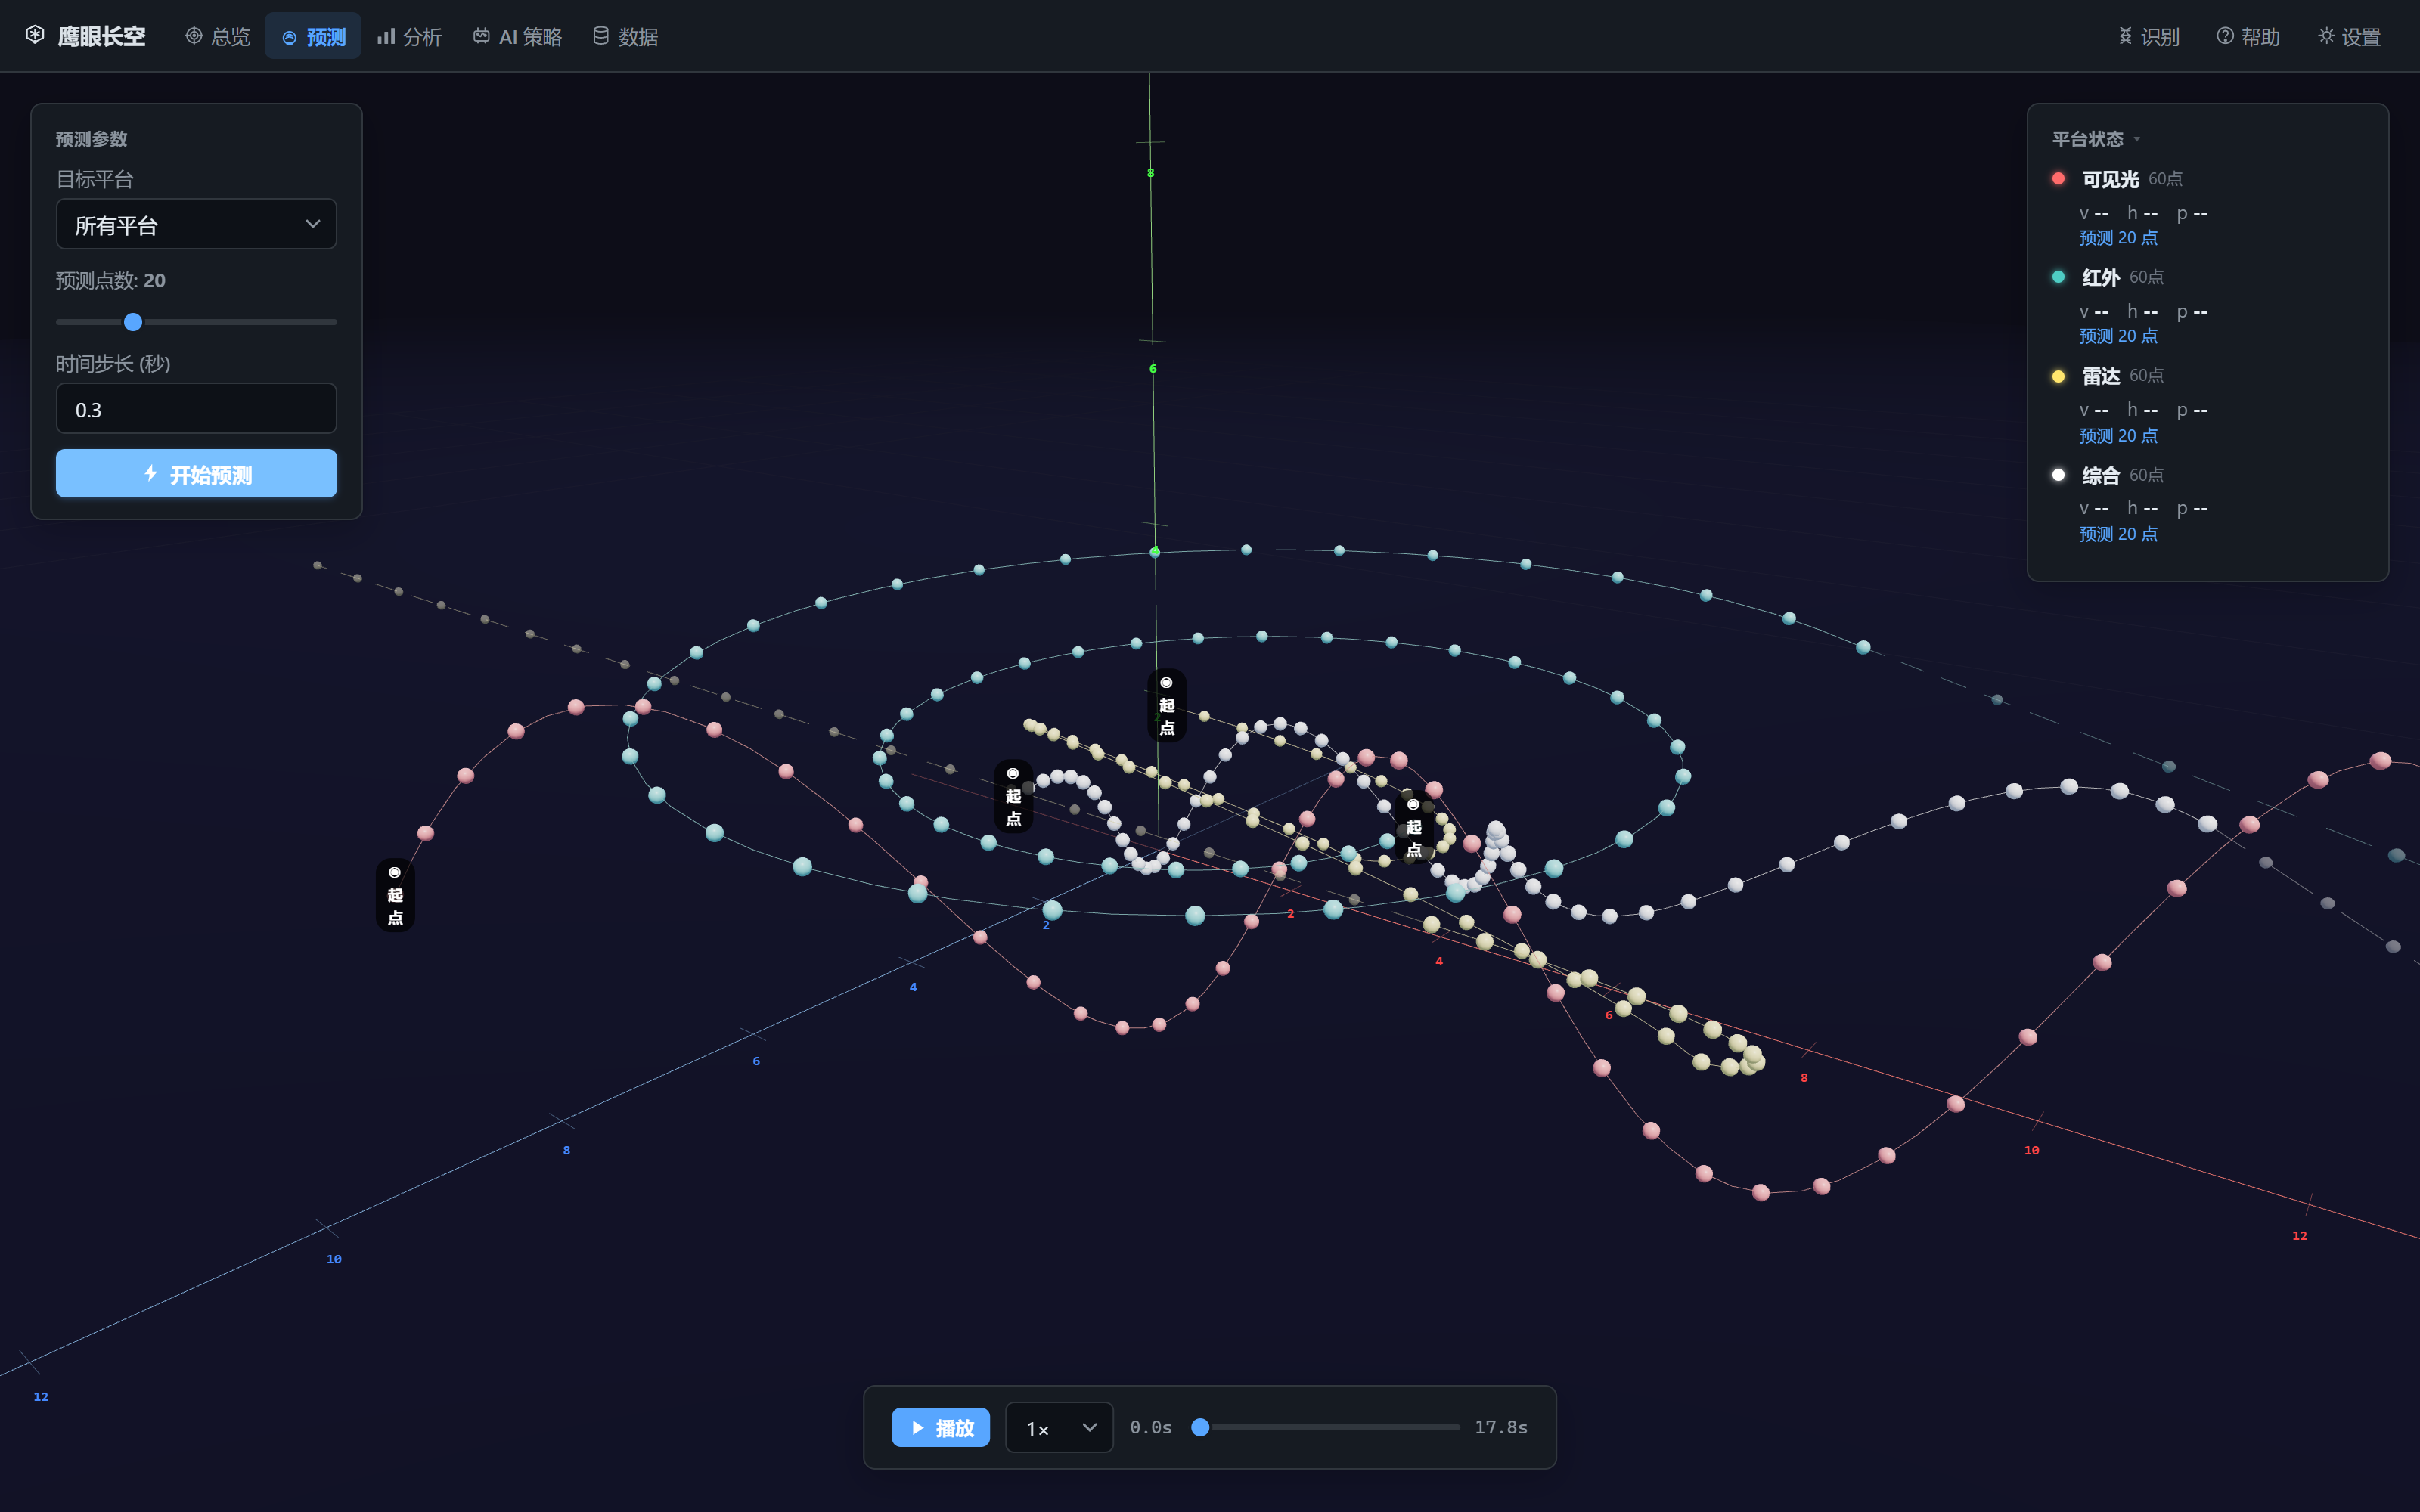
\includegraphics[width=\linewidth]{figures/ui/predict.png}};
\begin{scope}[x={(im.south east)},y={(im.north west)}]
  \hotspot{1}{0.133}{0.848}
  \hotspot{2}{0.133}{0.735}
  \hotspot{3}{0.960}{0.880}
  \hotspot{4}{0.170}{0.600}
  \hotspot{5}{0.335}{0.055}
\end{scope}
\end{tikzpicture}
\caption{预测页操作区域：\cn{1}~目标平台\quad \cn{2}~预测点数与步长\quad \cn{3}~平台状态（含预测点数）\quad \cn{4}~预测段（虚线）\quad \cn{5}~回放控制条}
\label{fig:use_predict}
\end{figure}

操作步骤：

\begin{enumerate}
  \item 在“目标平台”中选择单个平台或“所有平台”（\cn{1}）；
  \item 拖动“预测点数”滑块（10--50，默认 20），填写“时间步长”（默认 0.3 s）（\cn{2}）；
  \item 点击“开始预测”，场景中出现虚线预测段（\cn{4}），右上状态面板出现“预测 20 点”标注（\cn{3}）；
  \item 点击“播放”（\cn{5}），观察目标从历史段进入预测段的过渡是否平滑。
\end{enumerate}

\begin{notebox}[预测精度说明]
当前预测以线性外推兜底，即按最后两点的速度直线延伸，对转弯、加速等机动的描述能力有限；深度学习混合模型仍在完善中。预测结果适合判断大致走向，不宜作为精确拦截依据。
\end{notebox}

\subsubsection{分析页}

分析页把轨迹拆成四条曲线，并给出最适宜处置的三个时刻（图~\ref{fig:use_analysis}）。

\begin{figure}[H]
\centering
\begin{tikzpicture}
\node[inner sep=0, anchor=south west] (im) at (0,0)
  {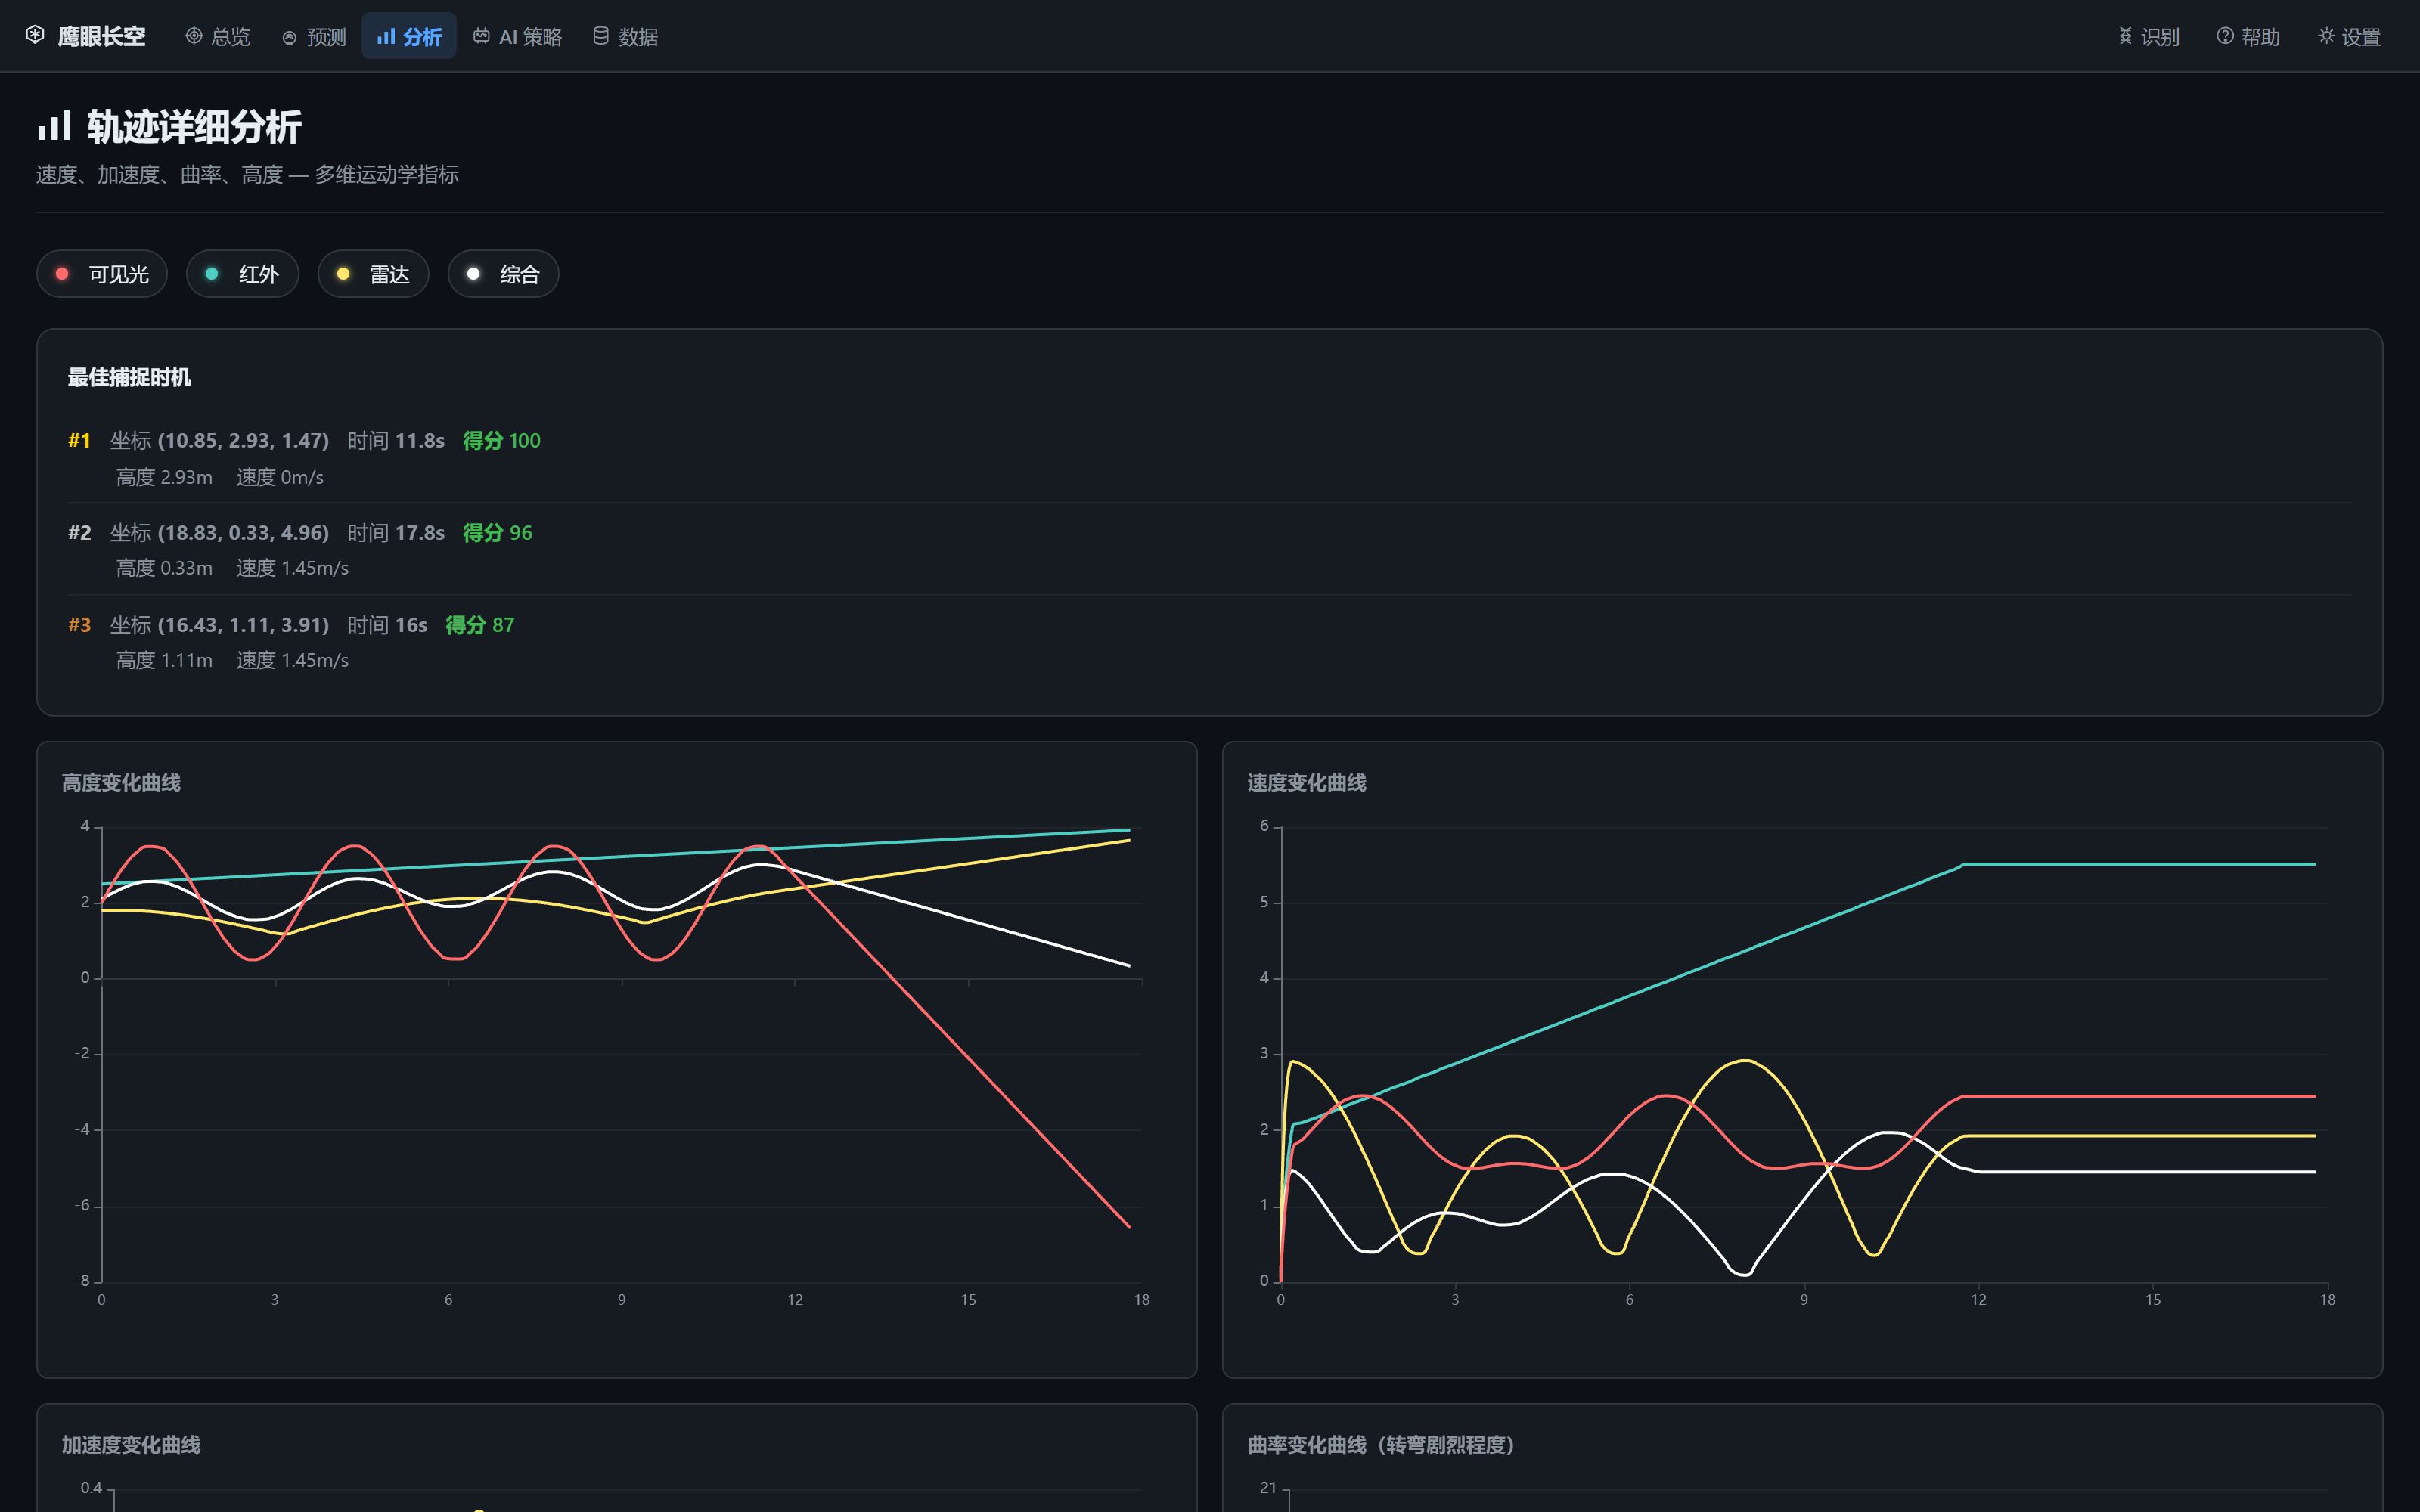
\includegraphics[width=\linewidth]{figures/ui/analysis.png}};
\begin{scope}[x={(im.south east)},y={(im.north west)}]
  \hotspot{1}{0.300}{0.805}
  \hotspot{2}{0.600}{0.720}
  \hotspot{3}{0.440}{0.600}
  \hotspot{4}{0.945}{0.600}
\end{scope}
\end{tikzpicture}
\caption{分析页操作区域：\cn{1}~平台筛选\quad \cn{2}~最佳捕捉时机\quad \cn{3}~高度/速度曲线\quad \cn{4}~加速度/曲率曲线}
\label{fig:use_analysis}
\end{figure}

\begin{enumerate}
  \item \term{平台筛选（\cn{1}）}：点击彩色标签只看某一平台，便于横向对比；默认全部显示。
  \item \term{最佳捕捉时机（\cn{2}）}：列出得分前三的时刻、坐标、得分（最高 100）、高度与速度；“越低、越慢、越平稳、航线越直”得分越高。
  \item \term{高度/速度曲线（\cn{3}）}：曲线末端为预测段，若出现陡降或突跳，说明预测偏离物理常识，应谨慎采信。
  \item \term{加速度/曲率曲线（\cn{4}）}：两者同时出现峰值，通常表示目标正在急转机动。
\end{enumerate}

\begin{notebox}[使用前提]
捕捉时机依赖预测数据：需先在预测页执行一次预测，否则该卡片为空。切换页面或重启后预测文件会被清空，需重新预测。
\end{notebox}

\subsubsection{AI 策略页}

AI 策略页把勾选平台的轨迹提交大模型，生成反制建议（图~\ref{fig:use_ai}）。

\begin{figure}[H]
\centering
\begin{tikzpicture}
\node[inner sep=0, anchor=south west] (im) at (0,0)
  {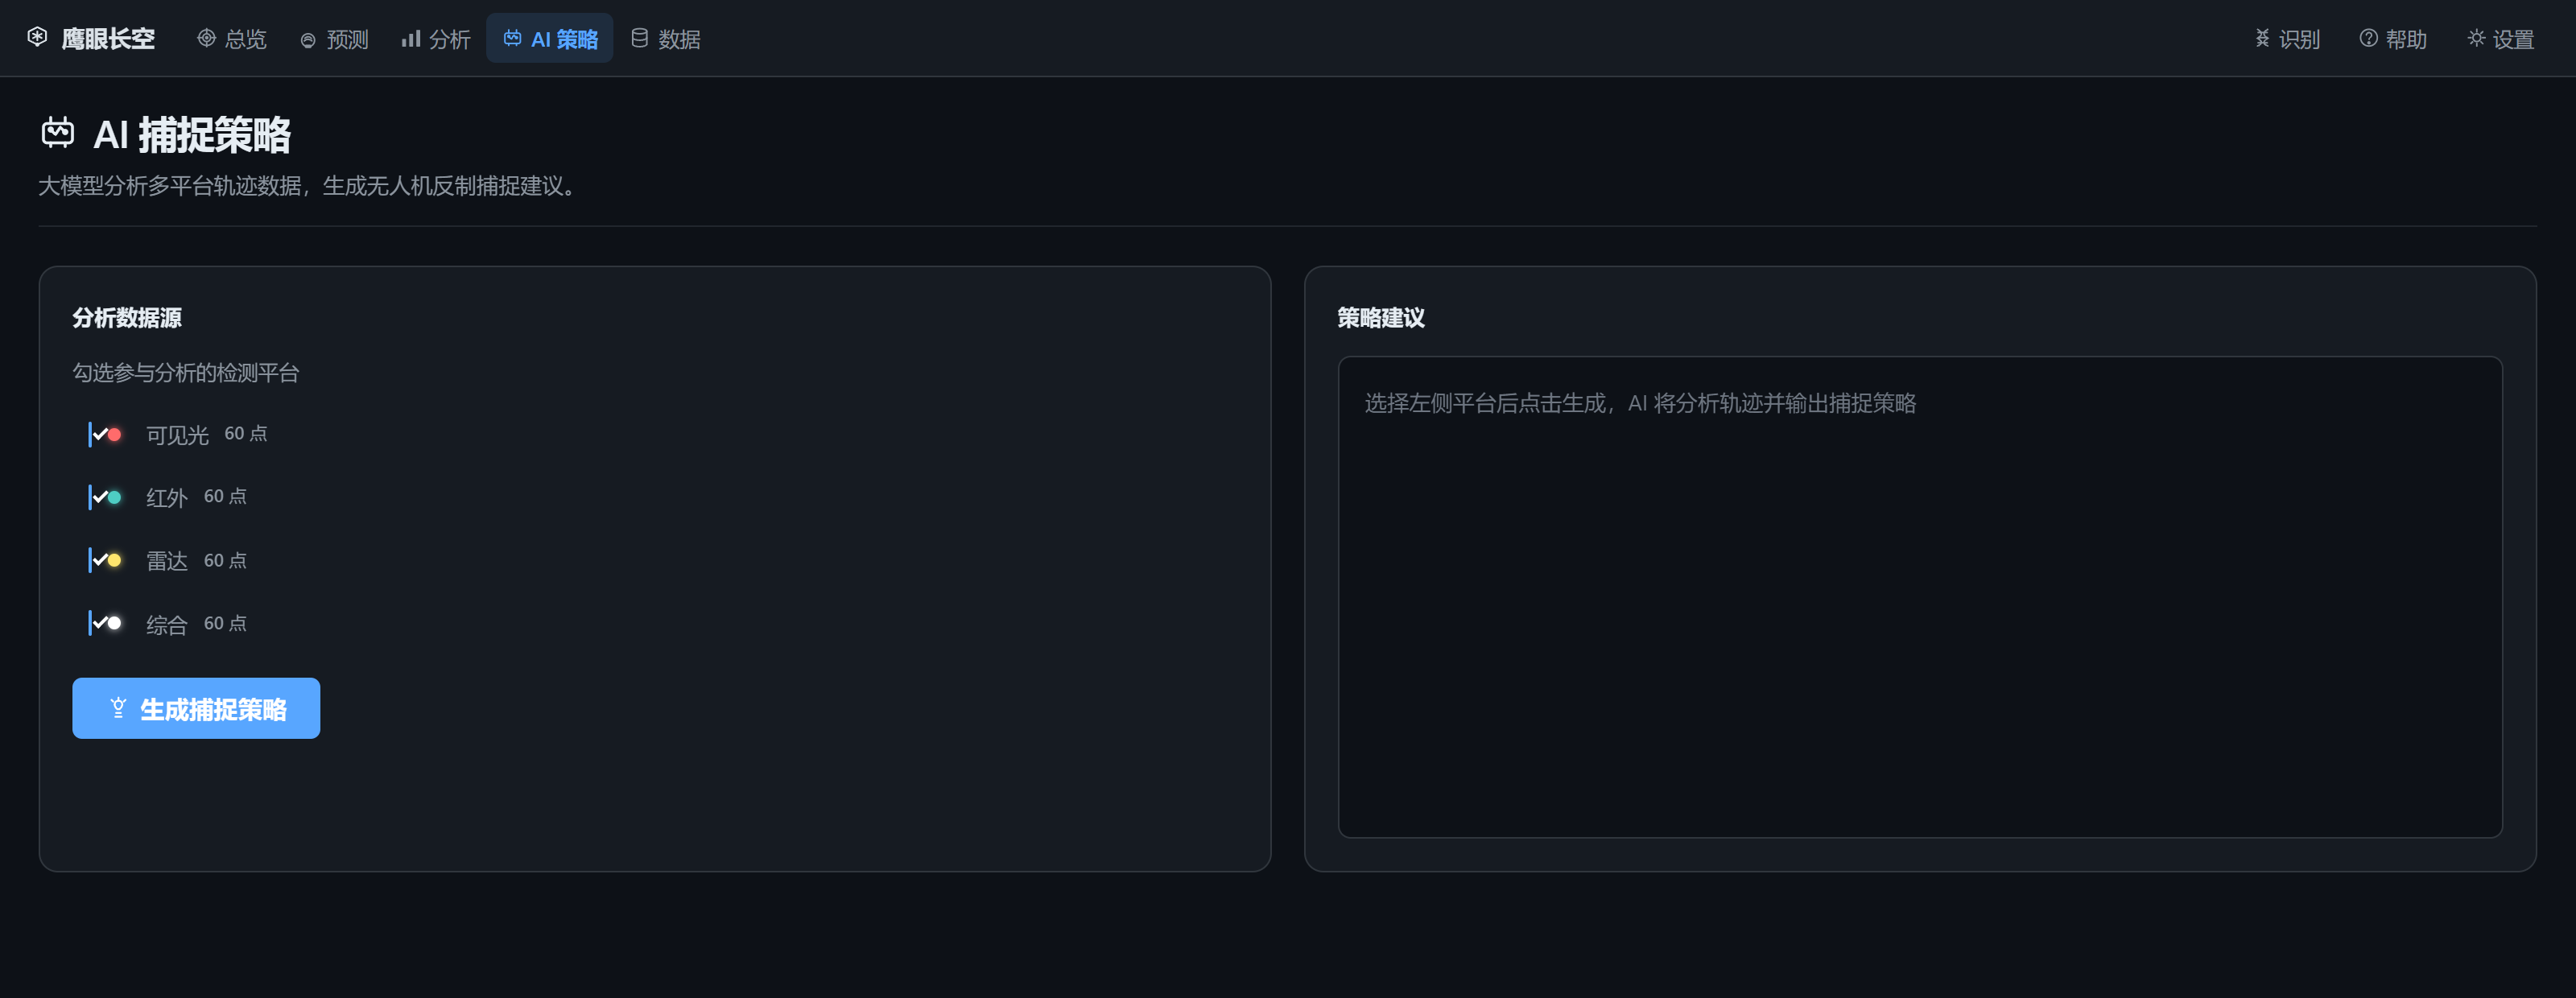
\includegraphics[width=\linewidth]{figures/ui/ai.png}};
\begin{scope}[x={(im.south east)},y={(im.north west)}]
  \hotspot{1}{0.300}{0.520}
  \hotspot{2}{0.155}{0.320}
  \hotspot{3}{0.800}{0.300}
\end{scope}
\end{tikzpicture}
\caption{AI 策略页操作区域：\cn{1}~平台勾选\quad \cn{2}~生成按钮\quad \cn{3}~策略输出区}
\label{fig:use_ai}
\end{figure}

\begin{enumerate}
  \item 勾选参与分析的平台（\cn{1}），建议一次勾选 2--3 个，避免提示词过长；
  \item 点击“生成捕捉策略”（\cn{2}），等待期间按钮显示加载状态；
  \item 返回的建议显示在右侧（\cn{3}），可点击“保存为报告”存入 \file{reports/}，文件名带时间戳。
\end{enumerate}

若提示“AI 服务异常”，请先检查 \file{config.json} 中 \code{ai} 段的地址、密钥与模型名，并确认网络可访问该接口。

\subsubsection{数据管理页}

数据页负责数据上传与备份恢复（图~\ref{fig:use_data}）。

\begin{figure}[H]
\centering
\begin{tikzpicture}
\node[inner sep=0, anchor=south west] (im) at (0,0)
  {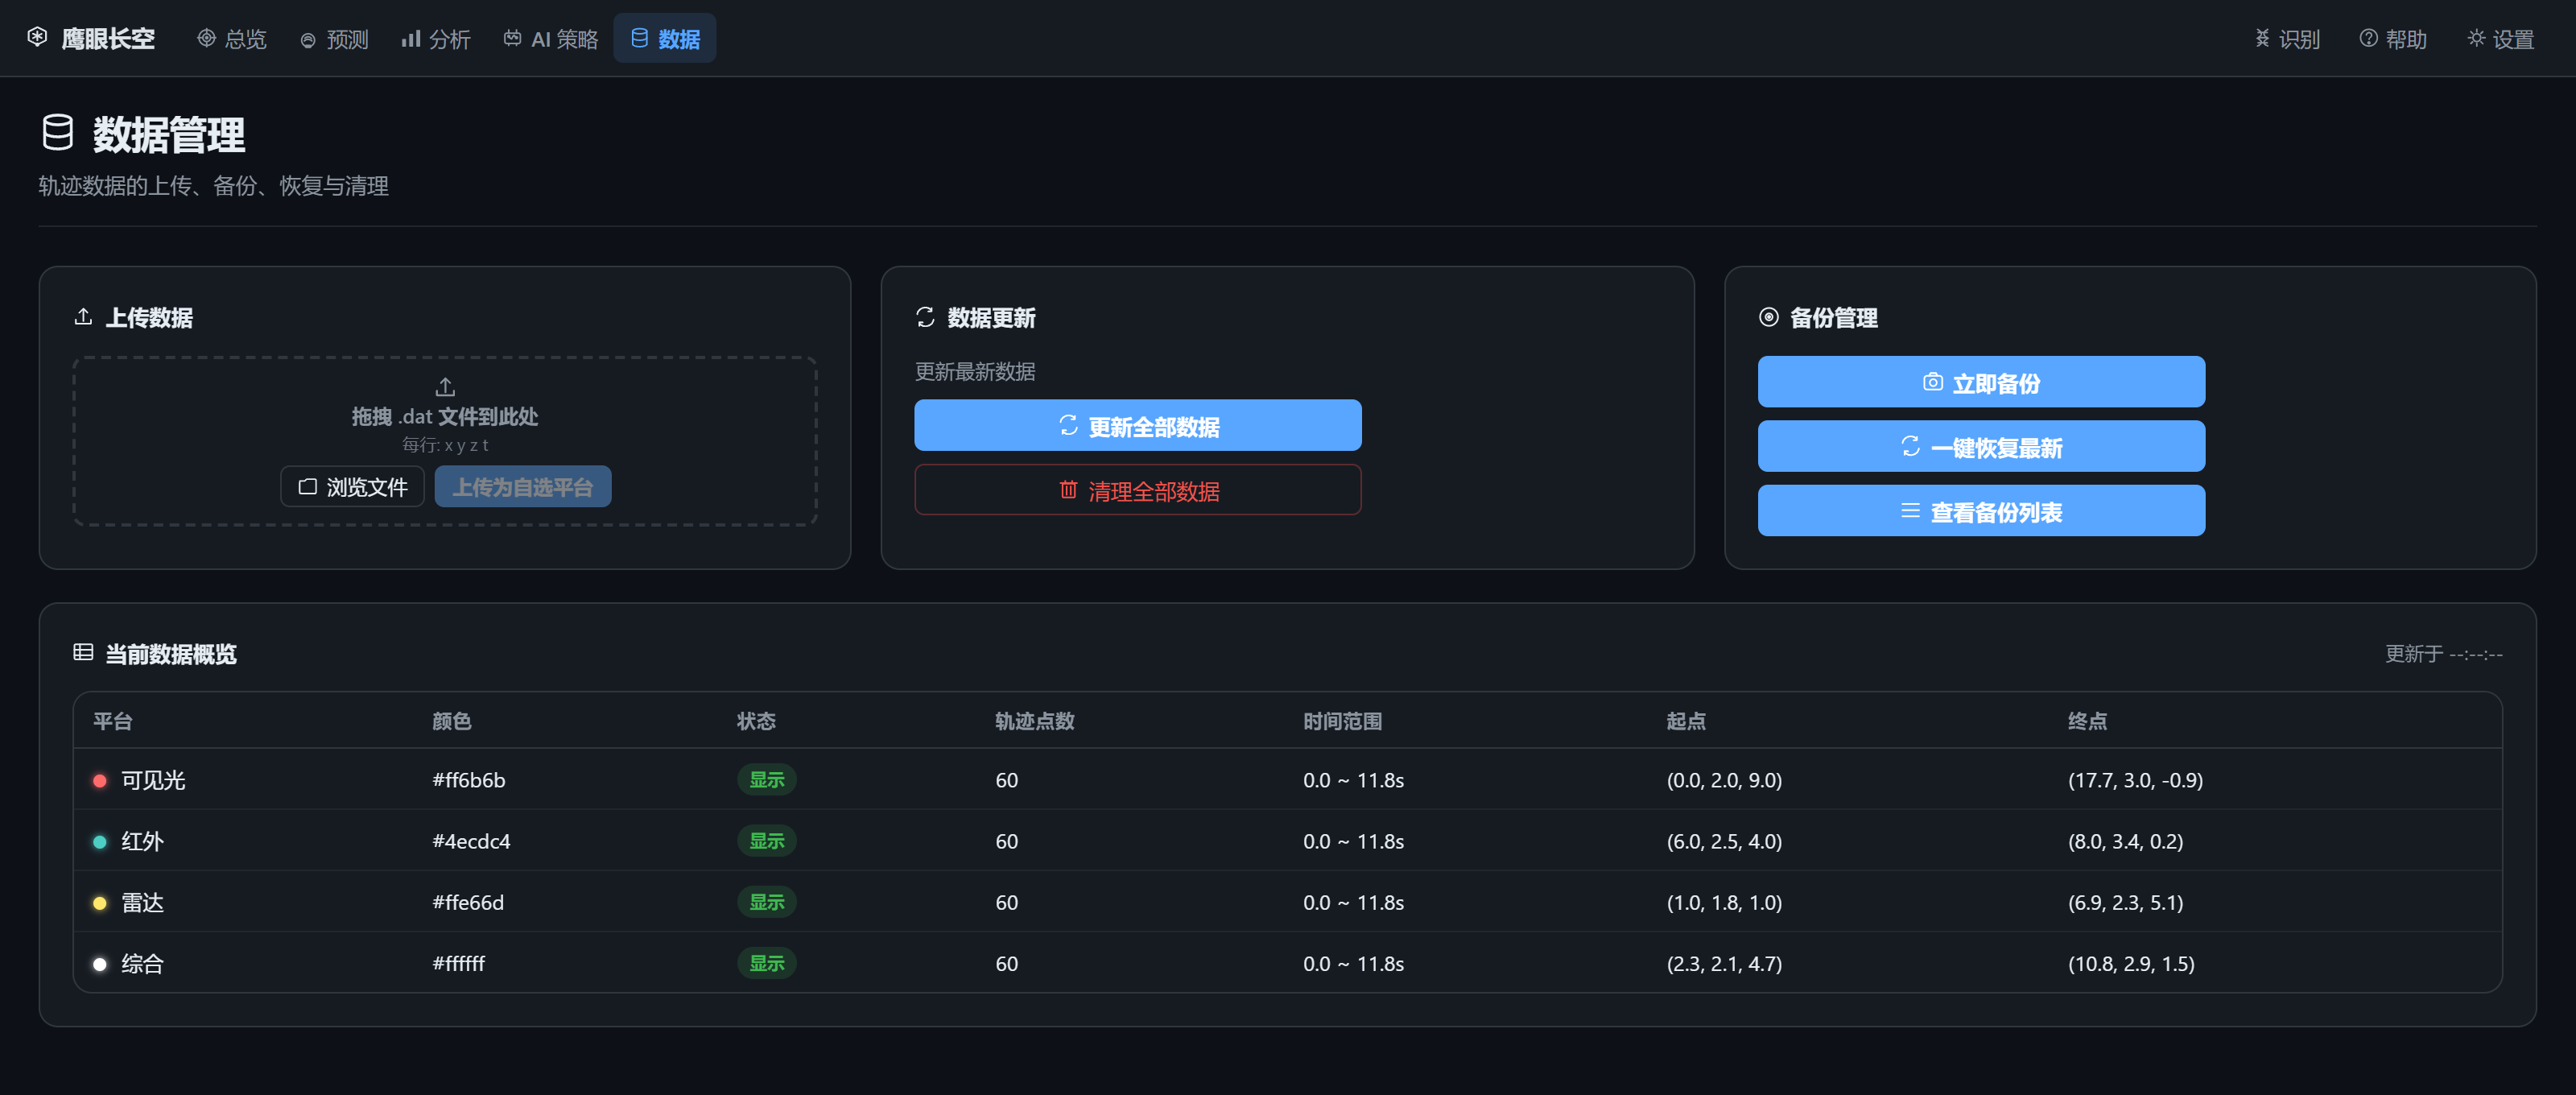
\includegraphics[width=\linewidth]{figures/ui/data.png}};
\begin{scope}[x={(im.south east)},y={(im.north west)}]
  \hotspot{1}{0.315}{0.815}
  \hotspot{2}{0.635}{0.815}
  \hotspot{3}{0.955}{0.815}
  \hotspot{4}{0.145}{0.400}
\end{scope}
\end{tikzpicture}
\caption{数据管理页操作区域：\cn{1}~上传自选数据\quad \cn{2}~数据更新与清理\quad \cn{3}~备份管理\quad \cn{4}~数据概览}
\label{fig:use_data}
\end{figure}

\begin{enumerate}
  \item \term{上传自选数据（\cn{1}）}：把每行 \code{x y z t} 的 \file{.dat} 文件拖入虚线框，或点击“浏览文件”；成功后出现新的“自选”平台。
  \item \term{数据更新与清理（\cn{2}）}：“更新全部数据”重新读取事实轨迹并重算综合轨迹；“清理全部数据”会先自动备份再清空，用于演示复位。
  \item \term{备份管理（\cn{3}）}：“立即备份”生成快照；“一键恢复最新”回到最近快照；“查看备份列表”可做部分恢复或删除。
  \item \term{数据概览（\cn{4}）}：逐平台显示颜色、状态、点数、时间范围、起点与终点，用于核对数据。
\end{enumerate}

\begin{notebox}[两种恢复方式]
\term{部分恢复}只覆盖快照中存在的文件，适合找回单个平台；\term{完整恢复}先清空现有数据再释放快照，适合回到某个历史状态。恢复后软件自动重算综合轨迹。
\end{notebox}

\subsubsection{设置页}

设置页调整主题、平台权重与评分权重（图~\ref{fig:use_settings}）。

\begin{figure}[H]
\centering
\begin{tikzpicture}
\node[inner sep=0, anchor=south west] (im) at (0,0)
  {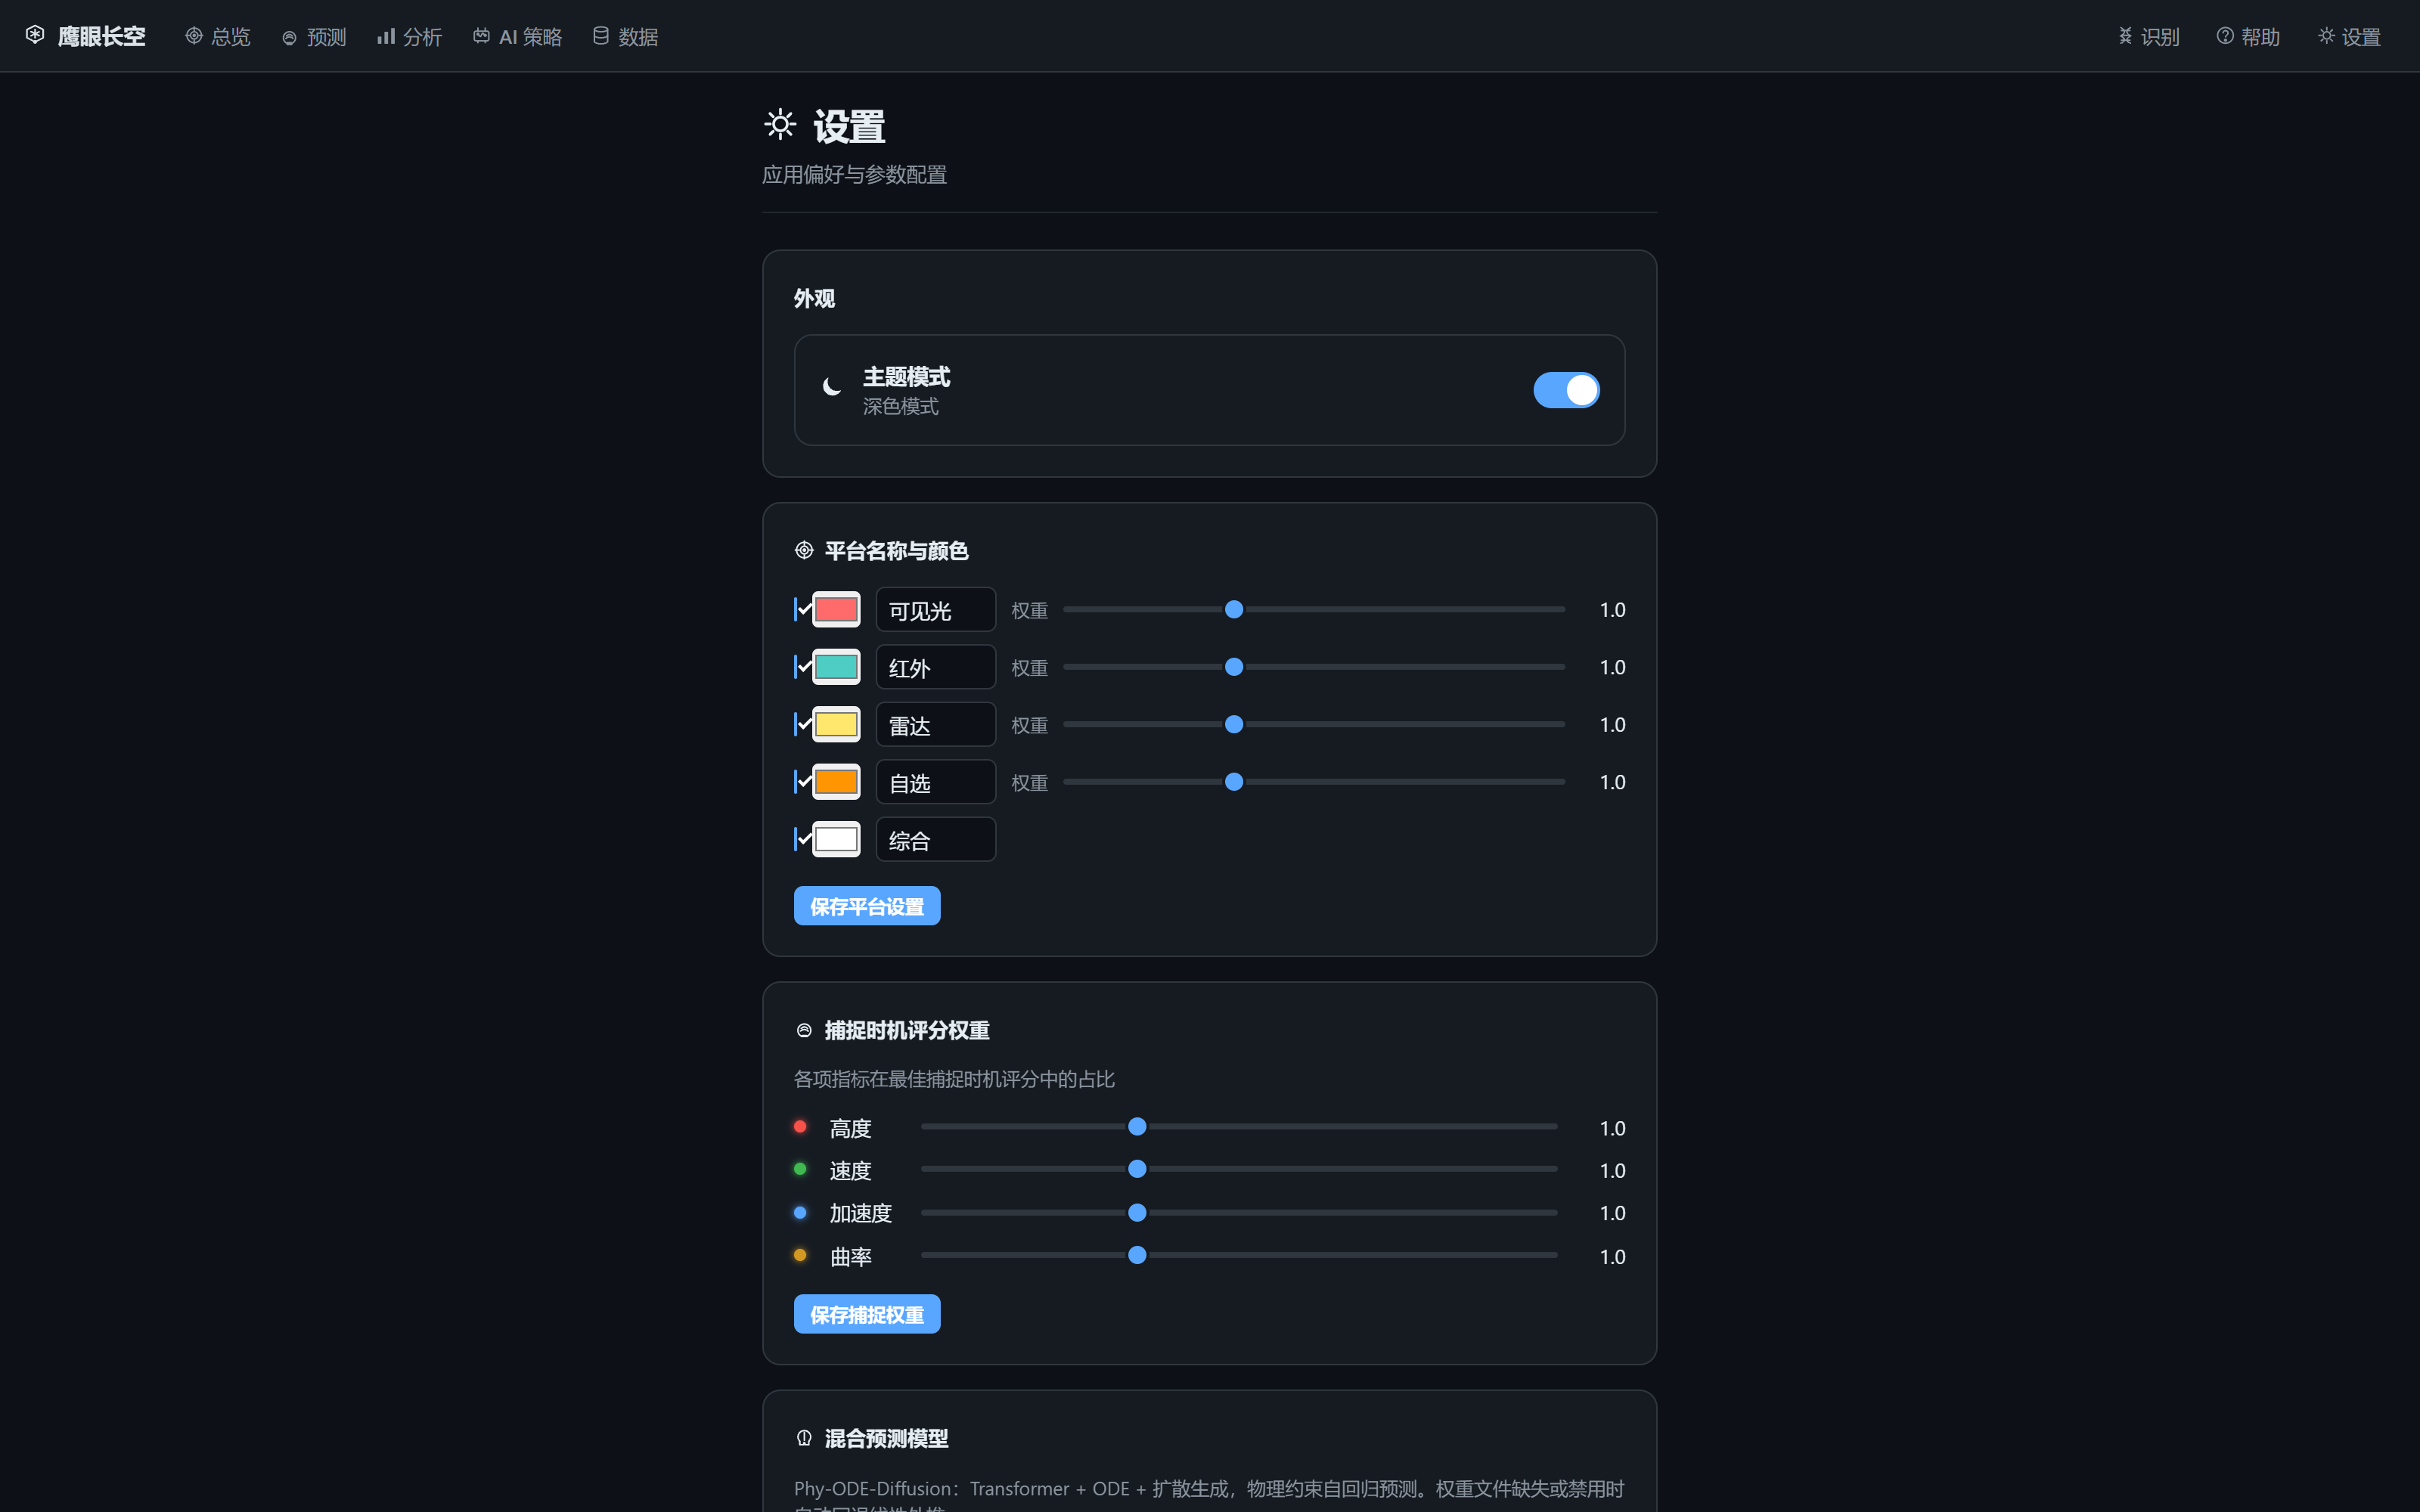
\includegraphics[width=\linewidth]{figures/ui/settings.png}};
\begin{scope}[x={(im.south east)},y={(im.north west)}]
  \hotspot{1}{0.600}{0.800}
  \hotspot{2}{0.600}{0.630}
  \hotspot{3}{0.600}{0.310}
\end{scope}
\end{tikzpicture}
\caption{设置页操作区域：\cn{1}~主题切换\quad \cn{2}~平台名称、颜色与权重\quad \cn{3}~捕捉评分权重}
\label{fig:use_settings}
\end{figure}

\begin{enumerate}
  \item \term{主题切换（\cn{1}）}：深色/浅色一键切换，立即生效并记住选择。
  \item \term{平台设置（\cn{2}）}：可改名称、颜色与融合权重；权重越大对综合轨迹影响越大，设为 0 即不参与融合。
  \item \term{捕捉权重（\cn{3}）}：调整高度、速度、加速度、曲率在评分中的比重，例如更看重低空就调大高度权重。
\end{enumerate}

设置页下方的“混合预测模型”区块用于调整最大速度、加速度、高度范围与推理步数等物理约束，保存后下一次预测生效。

\subsection{无人机检测的操作}

\subsubsection{检测工作台}

工作台自下而上分为视频源、检测控制、双目预览与实时信息四部分（图~\ref{fig:use_detect}）。

\begin{figure}[H]
\centering
\begin{tikzpicture}
\node[inner sep=0, anchor=south west] (im) at (0,0)
  {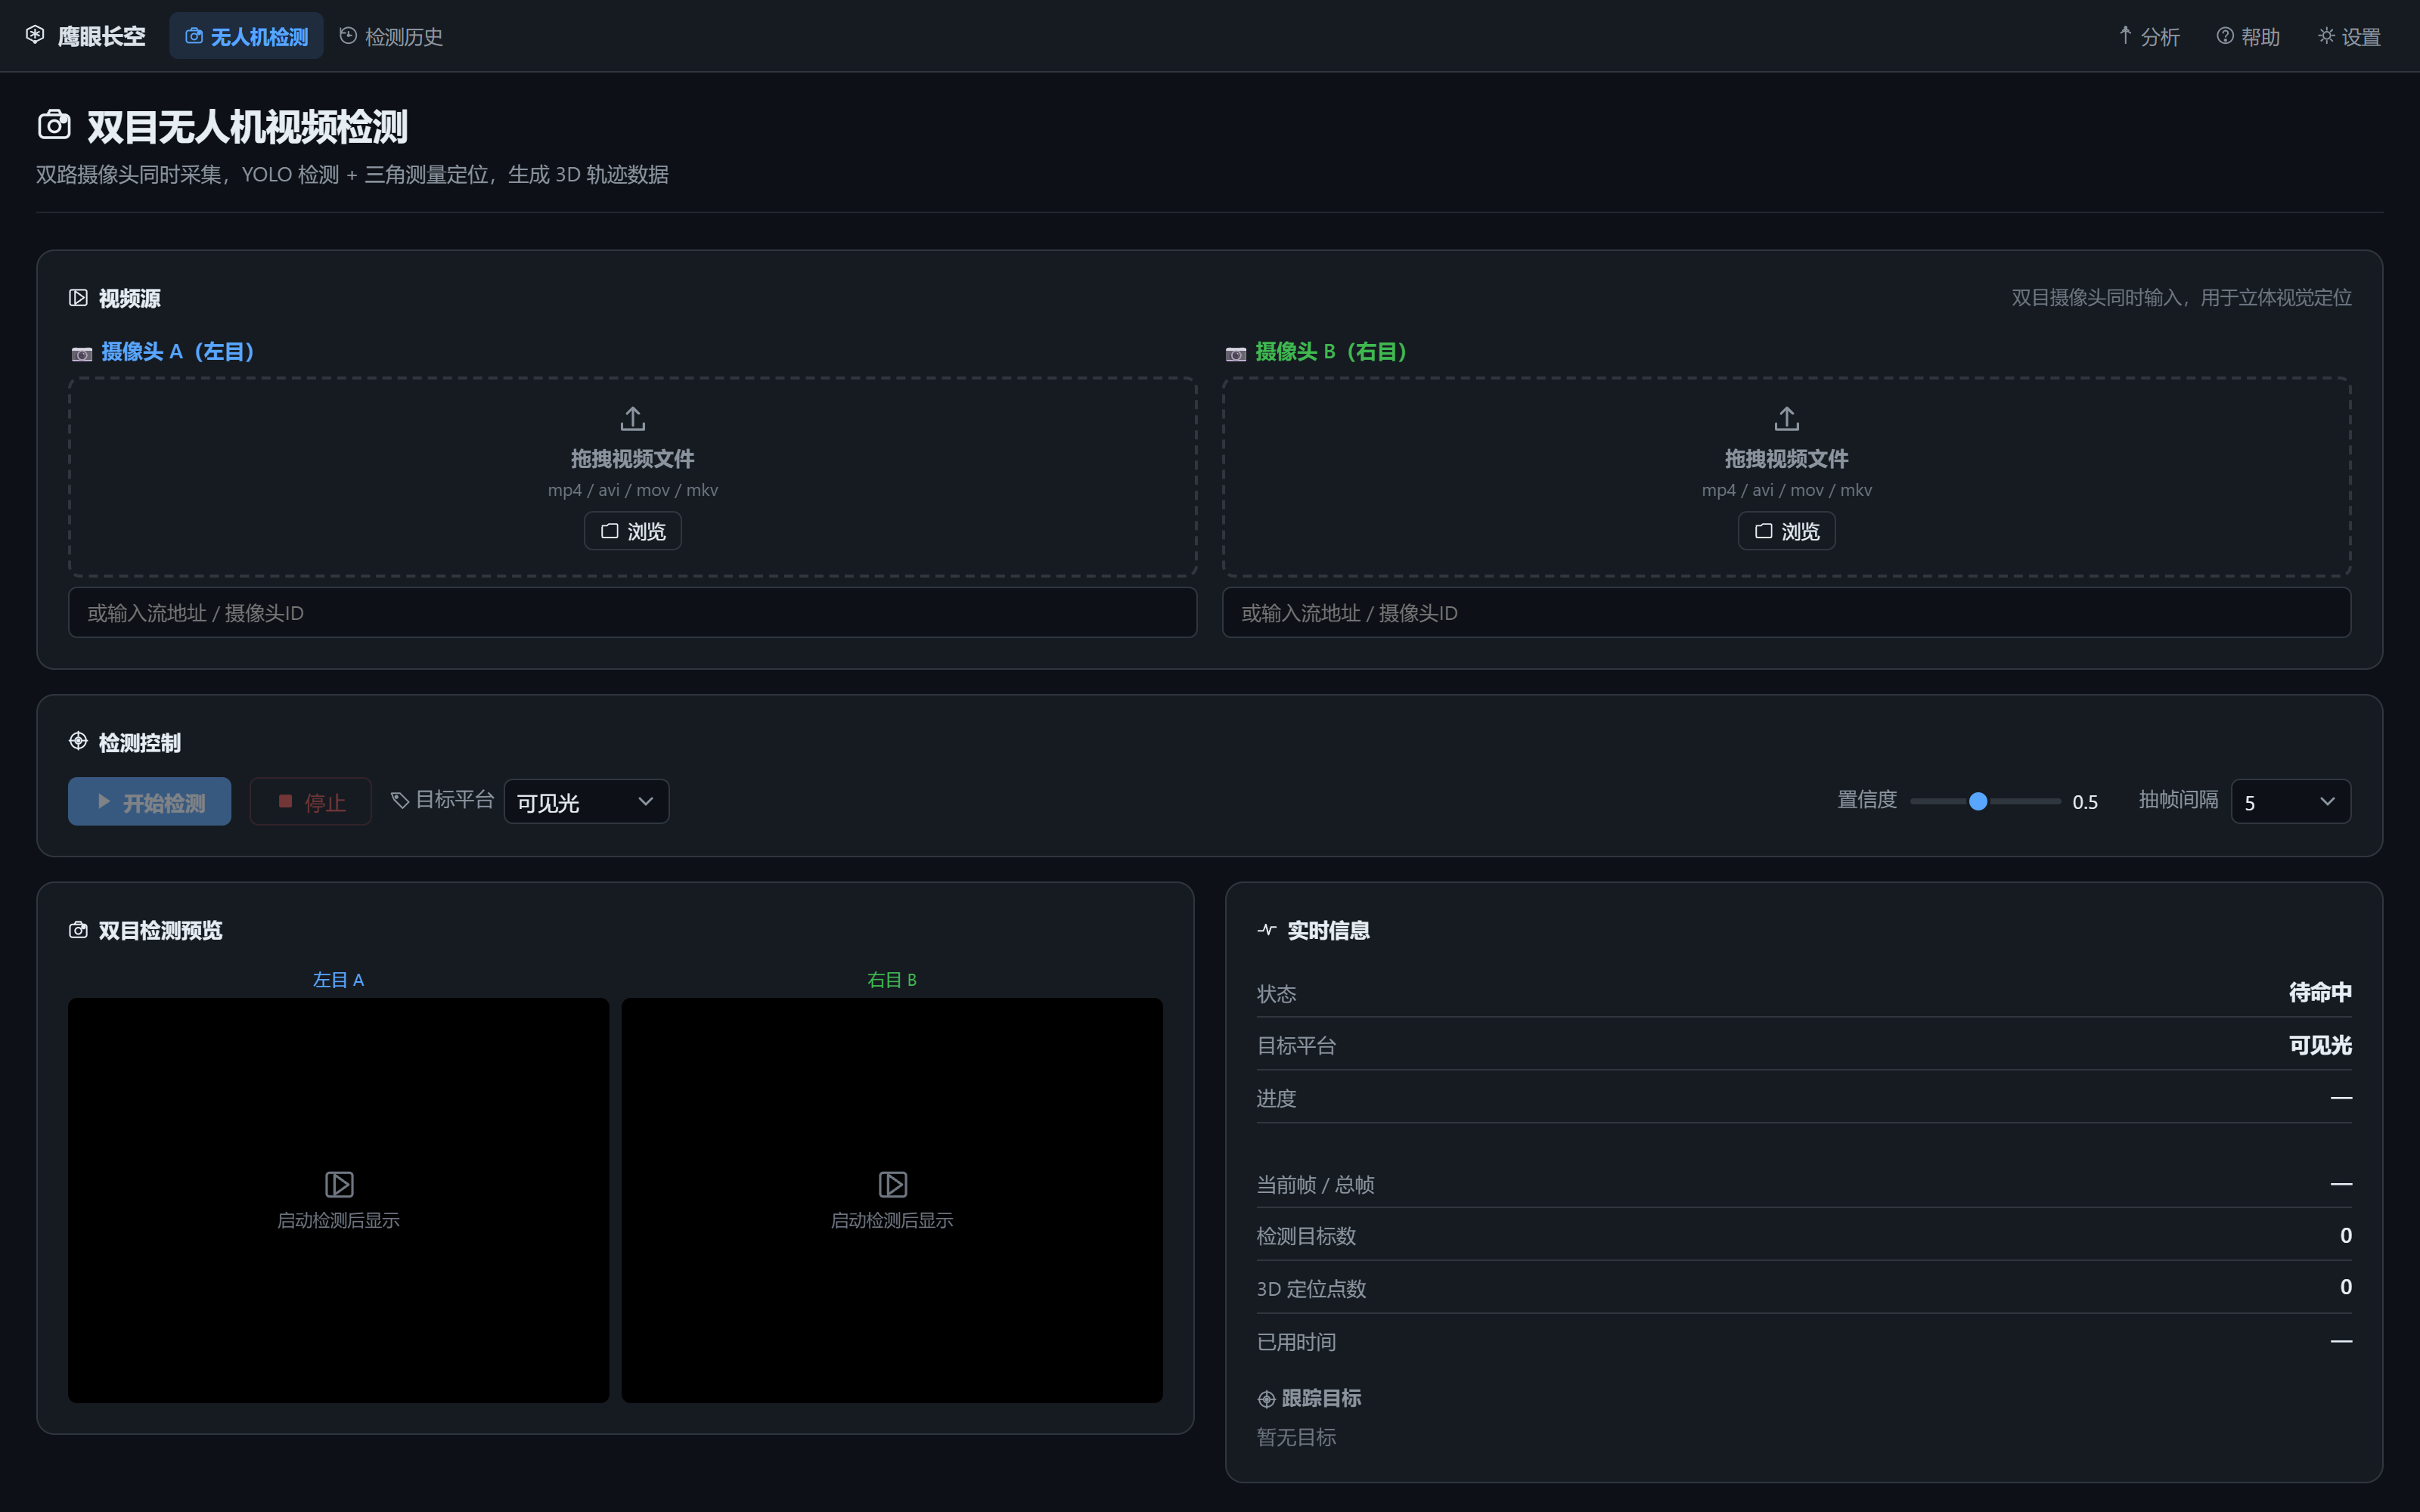
\includegraphics[width=\linewidth]{figures/ui/detect.png}};
\begin{scope}[x={(im.south east)},y={(im.north west)}]
  \hotspot{1}{0.300}{0.810}
  \hotspot{2}{0.350}{0.490}
  \hotspot{3}{0.440}{0.395}
  \hotspot{4}{0.945}{0.395}
\end{scope}
\end{tikzpicture}
\caption{检测工作台操作区域：\cn{1}~视频源上传\quad \cn{2}~检测控制条\quad \cn{3}~双目预览\quad \cn{4}~实时信息面板}
\label{fig:use_detect}
\end{figure}

\begin{enumerate}
  \item \term{视频源（\cn{1}）}：左右目各一个虚线框，可拖入视频文件（mp4/avi/mov/mkv），也可在下方填写 RTSP/HTTP 流地址或摄像头编号（如 \code{0}、\code{1}）。两路视频应来自同一时刻的双目相机，分辨率与帧率尽量一致。
  \item \term{检测控制（\cn{2}）}：开始/停止按钮、目标平台选择、置信度滑块与抽帧间隔；置信度越低越易检出但误检增多，抽帧间隔越大处理越快、轨迹越疏。
  \item \term{双目预览（\cn{3}）}：并排显示左右目画面，检测框上标注“类别 + 置信度”。
  \item \term{实时信息（\cn{4}）}：显示状态、进度、当前帧/总帧、目标数、三维点数、已用时与跟踪目标列表。
\end{enumerate}

操作步骤：拖入双路视频 → 选择目标平台 → 按需调整置信度与抽帧间隔 → 点击“开始检测” → 完成后点击“保存结果”（开启自动保存则无需此步）→ 回到总览页刷新即可看到新轨迹。

\begin{notebox}[检测没有结果怎么办]
先确认视频能正常播放；再检查设置页中的模型文件是否存在、目标类别是否与模型匹配；最后可把置信度调低到 0.1 重试。画面中明显有目标却完全没有框，多半是类别不匹配。
\end{notebox}

\subsubsection{检测设置}

\begin{figure}[H]
\centering
\begin{tikzpicture}
\node[inner sep=0, anchor=south west] (im) at (0,0)
  {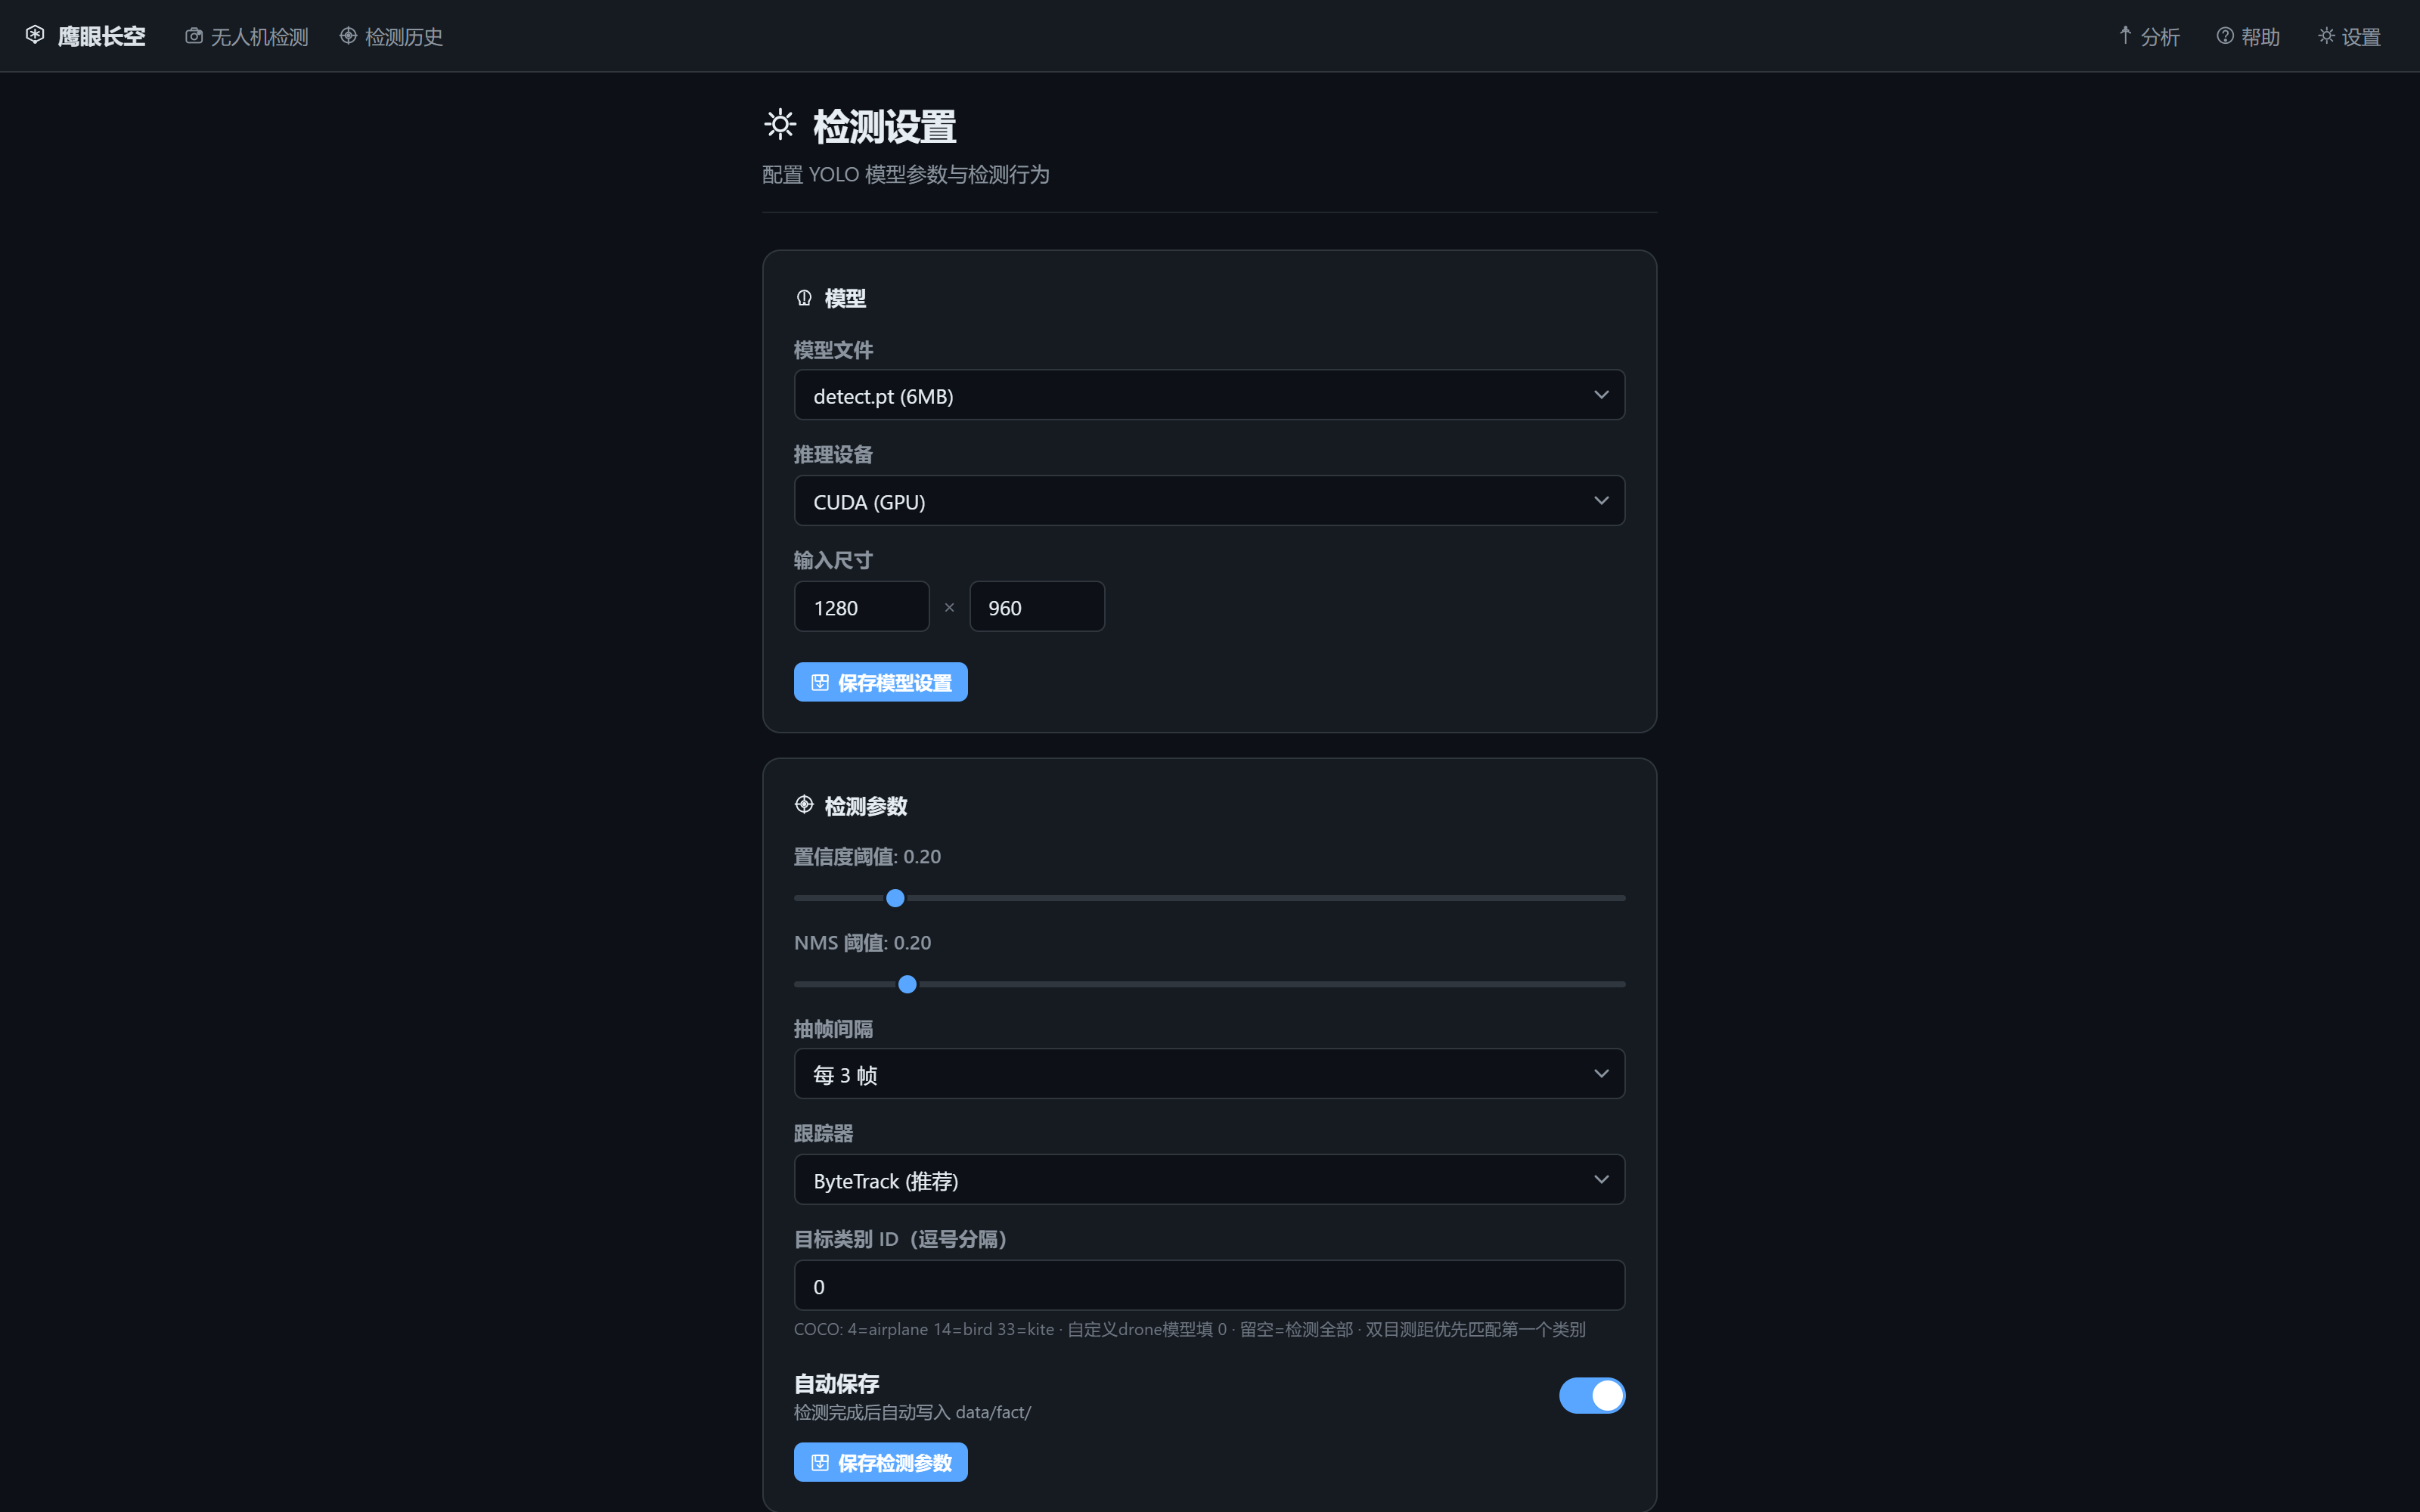
\includegraphics[width=\linewidth]{figures/ui/detect_settings.png}};
\begin{scope}[x={(im.south east)},y={(im.north west)}]
  \hotspot{1}{0.600}{0.800}
  \hotspot{2}{0.600}{0.470}
  \hotspot{3}{0.580}{0.080}
\end{scope}
\end{tikzpicture}
\caption{检测设置页操作区域：\cn{1}~模型与设备\quad \cn{2}~检测参数\quad \cn{3}~自动保存}
\label{fig:use_detect_settings}
\end{figure}

\begin{enumerate}
  \item \term{模型与设备（\cn{1}）}：选择 \file{models/yolo/} 中的权重；有 NVIDIA 显卡时选 CUDA 明显更快；输入尺寸一般保持 1280×960。
  \item \term{检测参数（\cn{2}）}：置信度、NMS、抽帧间隔、跟踪器与目标类别 ID。类别须与模型一致：自训练无人机模型通常为 0，COCO 预训练模型中飞机为 4、鸟为 14。
  \item \term{自动保存（\cn{3}）}：开启后检测完成即自动写入轨迹文件。
\end{enumerate}

修改后点击对应的“保存”按钮，参数立即写入 \file{config.json}，下一次检测生效。

\subsubsection{检测历史}

\begin{figure}[H]
\centering
\begin{tikzpicture}
\node[inner sep=0, anchor=south west] (im) at (0,0)
  {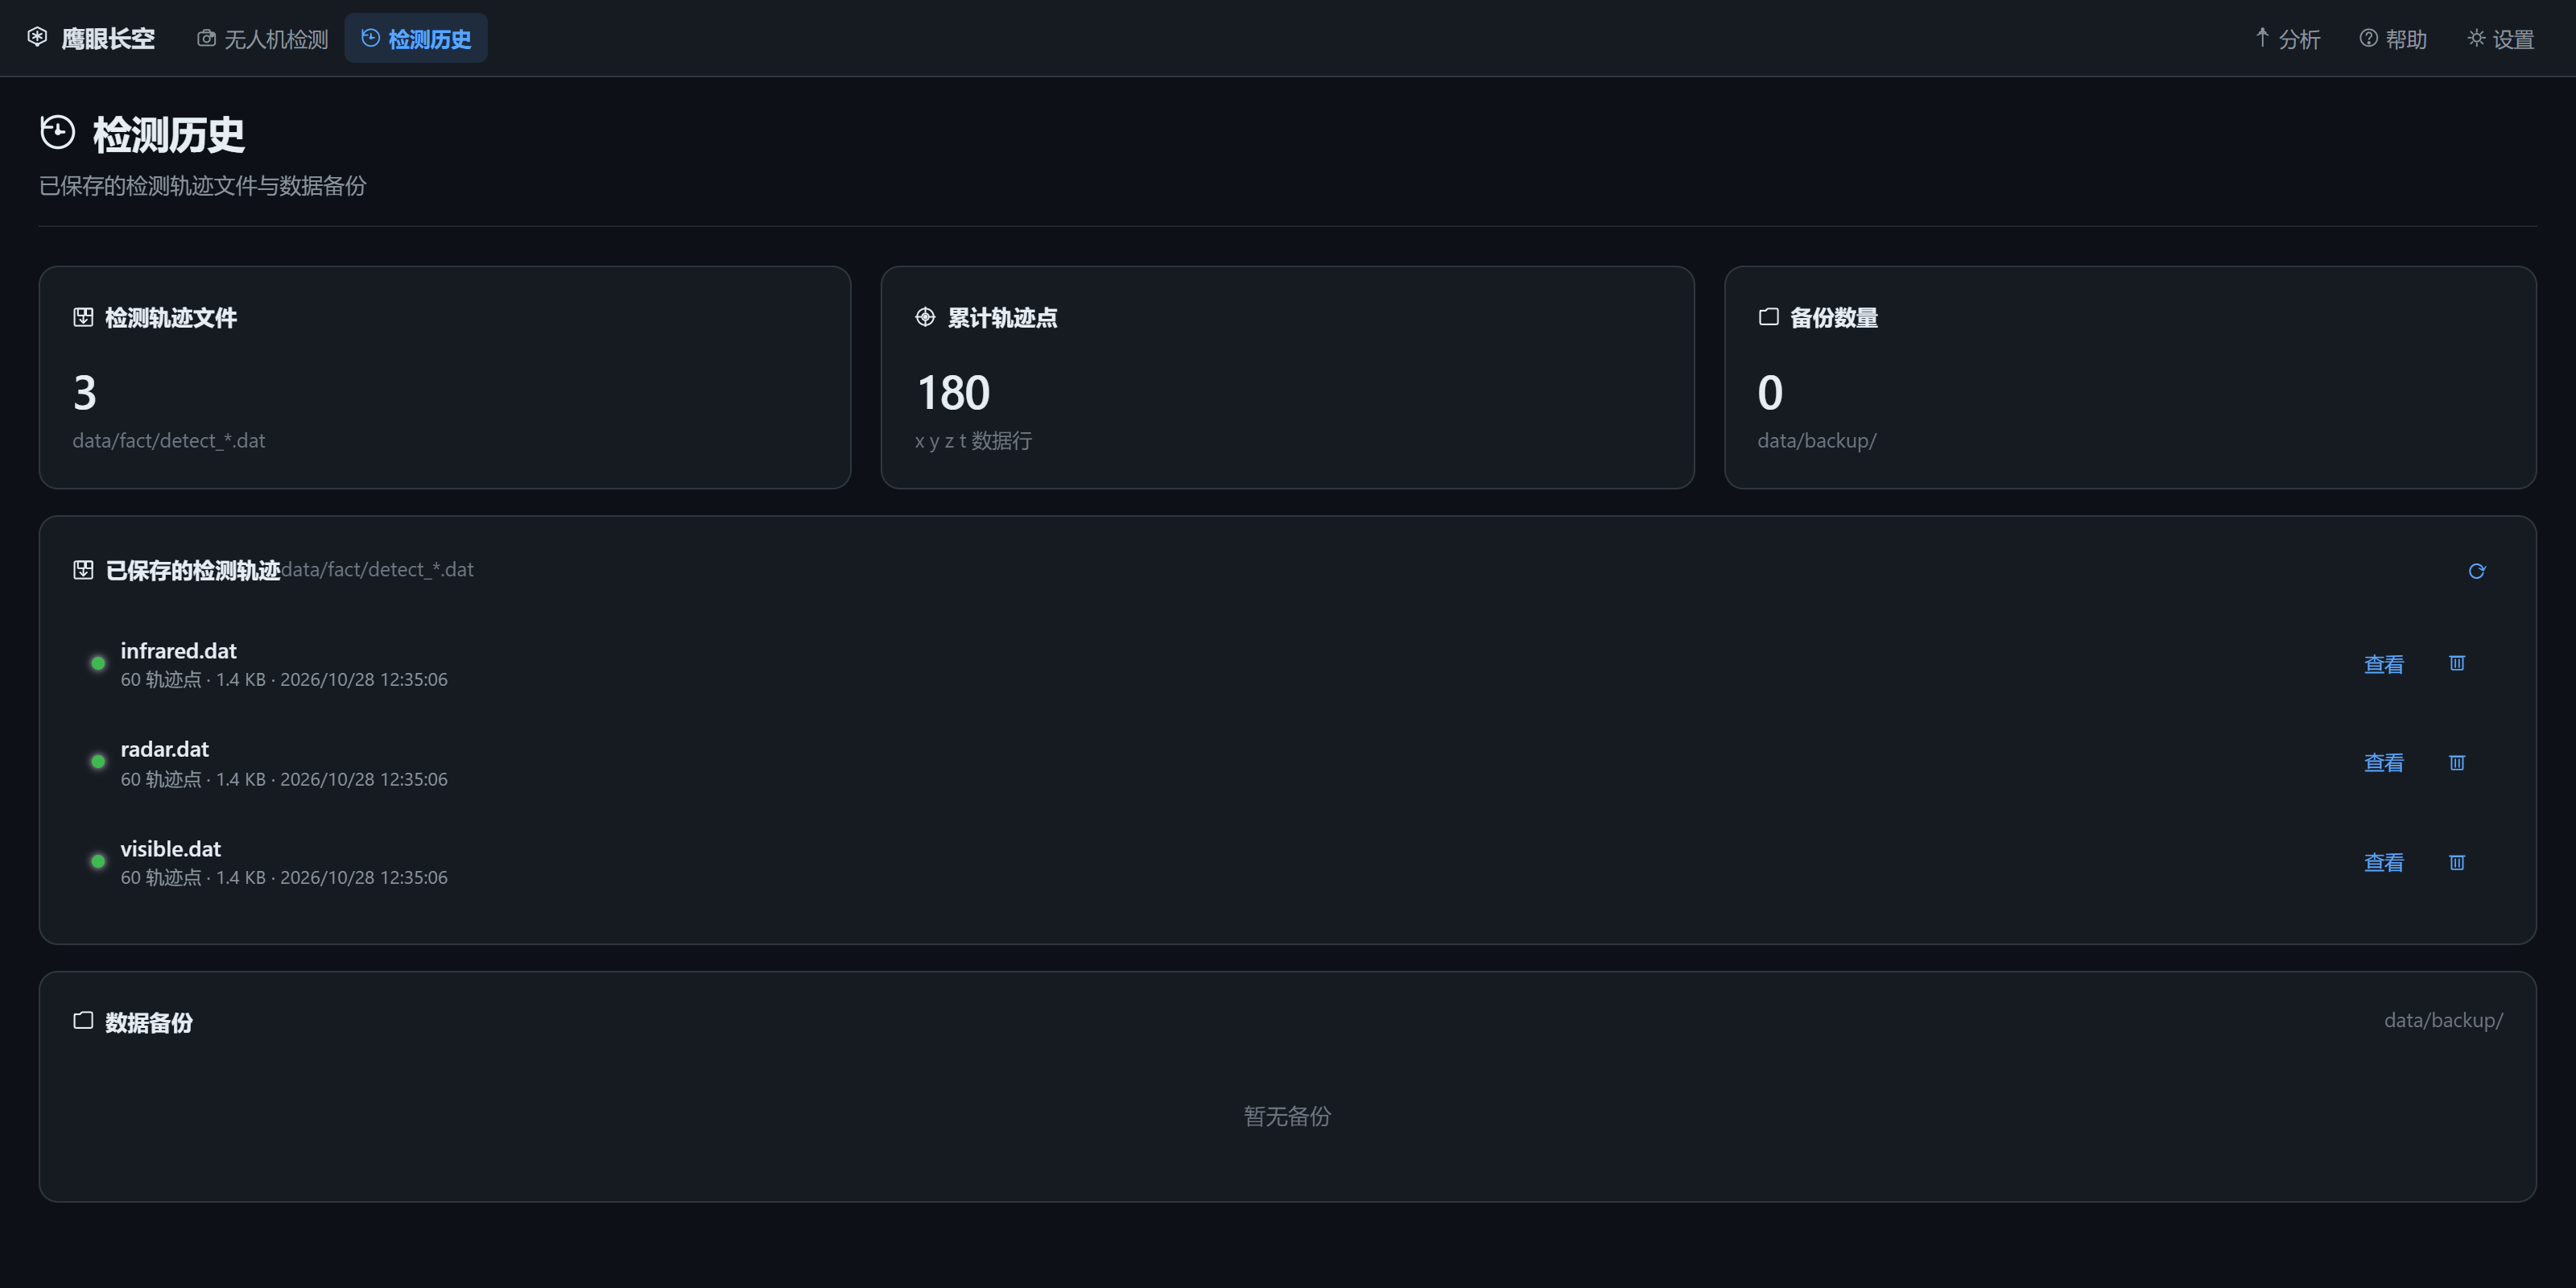
\includegraphics[width=\linewidth]{figures/ui/detect_history.png}};
\begin{scope}[x={(im.south east)},y={(im.north west)}]
  \hotspot{1}{0.300}{0.730}
  \hotspot{2}{0.945}{0.600}
  \hotspot{3}{0.945}{0.200}
\end{scope}
\end{tikzpicture}
\caption{检测历史页操作区域：\cn{1}~统计卡片\quad \cn{2}~轨迹文件列表\quad \cn{3}~备份列表}
\label{fig:use_detect_history}
\end{figure}

\begin{enumerate}
  \item \term{统计卡片（\cn{1}）}：轨迹文件数、累计轨迹点与备份数量。
  \item \term{轨迹文件列表（\cn{2}）}：显示平台名、点数、大小与修改时间，可查看或删除；删除前请确认已备份。
  \item \term{备份列表（\cn{3}）}：快照的时间、标签、文件数与点数；恢复操作在 5000 端口数据页完成，两个模块共用同一备份目录。
\end{enumerate}

\subsection{典型使用流程}

把常用操作串成三条流程，便于新用户按图索骥（图~\ref{fig:use_flow_view}--\ref{fig:use_flow_detect}）。

\begin{figure}[H]
\centering
\begin{tikzpicture}[node distance=6mm]
\node[term] (s) {启动软件};
\node[proc, below=6mm of s, text width=54mm] (p1) {打开总览页（5000）};
\node[proc, below=6mm of p1, text width=54mm] (p2) {按需隐藏/显示平台};
\node[proc, below=6mm of p2, text width=54mm] (p3) {旋转、缩放、平移视角};
\node[proc, below=6mm of p3, text width=54mm] (p4) {播放动画，悬停读点};
\node[term, below=6mm of p4] (e) {形成态势判断};
\foreach \a/\b in {s/p1,p1/p2,p2/p3,p3/p4,p4/e} \draw[arr] (\a) -- (\b);
\end{tikzpicture}
\caption{流程一：快速查看多平台态势}
\label{fig:use_flow_view}
\end{figure}

\begin{figure}[H]
\centering
\begin{tikzpicture}[node distance=6mm]
\node[term] (s) {总览页};
\node[proc, below=6mm of s, text width=58mm] (p1) {进入预测页，选平台与参数并预测};
\node[deci, below=7mm of p1] (d1) {预测成功};
\node[proc, below left=9mm and 6mm of d1, text width=46mm] (p2) {分析页看曲线与捕捉时机};
\node[proc, below right=9mm and 6mm of d1, text width=40mm] (p3) {调整点数/步长重试};
\node[proc, below=6mm of p2, text width=46mm] (p4) {AI 策略页生成建议};
\node[term, below=6mm of p4] (e) {形成处置建议};
\draw[arr] (s) -- (p1); \draw[arr] (p1) -- (d1);
\draw[arr] (d1.west) -| node[lbl, above, pos=0.7]{是} (p2.north);
\draw[arr] (d1.east) -| node[lbl, above, pos=0.7]{否} (p3.north);
\draw[arr] (p3.south) |- (p1.east);
\draw[arr] (p2) -- (p4); \draw[arr] (p4) -- (e);
\end{tikzpicture}
\caption{流程二：预测—分析—AI 策略}
\label{fig:use_flow_analyze}
\end{figure}

\begin{figure}[H]
\centering
\begin{tikzpicture}[node distance=6mm]
\node[term] (s) {检测工作台};
\node[proc, below=6mm of s, text width=62mm] (p1) {上传左右目视频或填写流地址};
\node[proc, below=6mm of p1, text width=62mm] (p2) {选平台，调置信度与抽帧间隔};
\node[proc, below=6mm of p2, text width=62mm] (p3) {开始检测，观察预览与进度};
\node[proc, below=6mm of p3, text width=62mm] (p4) {保存结果（或开启自动保存）};
\node[proc, below=6mm of p4, text width=62mm] (p5) {总览页刷新查看新轨迹};
\node[term, below=6mm of p5] (e) {轨迹可供预测与分析};
\foreach \a/\b in {s/p1,p1/p2,p2/p3,p3/p4,p4/p5,p5/e} \draw[arr] (\a) -- (\b);
\end{tikzpicture}
\caption{流程三：从视频检测到轨迹入库}
\label{fig:use_flow_detect}
\end{figure}

\subsection{常见问题速查}

\begin{table}[H]
\centering
\caption{常见问题与处理办法}
\label{tab:use_faq}
\small
\begin{tabularx}{\linewidth}{@{}>{\heiti}p{4.0cm}>{\raggedright\arraybackslash}X@{}}
\toprule
现象 & 原因与处理 \\
\midrule
提示端口被占用 & 程序会自动清理；仍失败时用 \code{netstat -ano | findstr :5000} 找到进程并结束 \\
页面空白或样式缺失 & 浏览器强制刷新（Ctrl+F5）；确认通过 5000/5001 地址进入 \\
桌面窗口打不开 & 缺少 WebView2 运行时；安装后重试，或改用 \code{--headless} 模式 \\
总览页没有轨迹 & \file{data/fact/} 无数据；到数据页点“更新全部数据”，或用检测模块生成 \\
分析页没有捕捉卡片 & 尚未预测；先到预测页执行一次预测 \\
预测段是一条直线 & 当前为线性外推兜底，属正常现象 \\
AI 策略报错 & 检查 \code{ai} 段配置与网络连通性 \\
检测没有检测框 & 类别不匹配或置信度偏高；调低置信度、核对 \code{target_classes} \\
检测速度慢 & 无 GPU 时单帧约 1.5 s；增大抽帧间隔或改用 CUDA 版 PyTorch \\
上传文件被拒 & 文件需为每行 \code{x y z t} 的文本，空格分隔、四列齐全 \\
配置损坏无法启动 & 删除 \file{config.json}，重启后按模板自动重建 \\
\bottomrule
\end{tabularx}
\end{table}

% ============================================================
%  第十一章  安装部署与运行
% ============================================================
\section{安装部署与运行}

\subsection{环境准备}

推荐使用 Conda 创建独立环境，避免与系统 Python 包冲突。本项目统一使用名为 \code{drone} 的环境：

\begin{lstlisting}[style=sh, caption={创建并激活虚拟环境}]
conda create -n drone python=3.11 -y
conda activate drone
\end{lstlisting}

选择 Python 3.11 的原因：PyTorch、OpenCV、ultralytics 等依赖在该版本上的预编译轮子最完整；过新的版本（如 3.13/3.14）常出现轮子缺失、需本地编译的问题。

\subsection{依赖安装}

\subsubsection{安装 PyTorch}

先安装与硬件匹配的 PyTorch，再安装其余依赖，可避免 pip 自动拉取不匹配的版本：

\begin{lstlisting}[style=sh, caption={PyTorch 安装（按硬件三选一）}]
# CPU 版本
pip install torch torchvision --index-url https://download.pytorch.org/whl/cpu

# NVIDIA GPU（CUDA 12.4）
pip install torch torchvision --index-url https://download.pytorch.org/whl/cu124

# NVIDIA GPU（CUDA 11.8）
pip install torch torchvision --index-url https://download.pytorch.org/whl/cu118
\end{lstlisting}

\subsubsection{安装其余依赖}

\begin{lstlisting}[style=sh, caption={安装项目依赖}]
cd D:\CodeWorks\drone
pip install -r requirements.txt
\end{lstlisting}

\file{requirements.txt} 的内容为：flask、requests、pywebview、ultralytics、opencv-python、numpy、tqdm、matplotlib。

\subsubsection{版本验证}

安装完成后执行自检：

\begin{lstlisting}[style=sh, caption={环境自检}]
python -c "import flask, cv2, torch, numpy, ultralytics, webview; \
print(flask.__version__, cv2.__version__, torch.__version__)"
\end{lstlisting}

本次文档编写环境实测的版本如表~\ref{tab:versions} 所示。

\begin{table}[H]
\centering
\caption{实测环境版本}
\label{tab:versions}
\small
\begin{tabularx}{\linewidth}{@{}>{\heiti}p{3.4cm}>{\ttfamily}p{4.2cm}>{\raggedright\arraybackslash}X@{}}
\toprule
组件 & 实测版本 & 说明 \\
\midrule
操作系统 & Windows 11（x64） & 亦支持 Windows 10 \\
Python & 3.11.17 & Conda 环境 \code{drone} \\
Flask & 3.1.3 & Web 框架 \\
PyTorch & 2.14.1+cpu & CPU 轮子，GPU 环境为 +cu124 \\
torchvision & 0.29.1+cpu & 与 PyTorch 配套 \\
OpenCV & 5.0.0 & 视频解码与图像处理 \\
NumPy & 2.4.6 & 数组与文件读写 \\
ultralytics & 8.4.191 & YOLO 推理与跟踪 \\
pywebview & 5.x & 桌面窗口（依赖 WebView2） \\
\bottomrule
\end{tabularx}
\end{table}

\begin{notebox}[WebView2 运行时]
Windows 11 已内置 WebView2 运行时；Windows 10 若缺少，需安装“Microsoft Edge WebView2 Runtime”。若不希望安装该运行时，可使用 \code{--headless} 模式，通过浏览器访问。
\end{notebox}

\subsection{模型与数据准备}

\begin{enumerate}
  \item \term{YOLO 权重}：放置在 \file{models/yolo/}，默认读取 \file{detect.pt}。首次使用 ultralytics 时若指定 \code{yolov8n.pt} 等官方名称，会自动从网络下载。
  \item \term{预测权重}：放置在 \file{models/kinflow/}（或训练产物 \file{train/kinflow_predictor/train_result/best/}）。按“\code{best_s2} $\rightarrow$ \code{best_s1}”的优先级选择；缺失时自动回退线性外推。
  \item \term{轨迹数据}：\file{data/fact/} 下的 \file{visible.npz}、\file{infrared.npz}、\file{radar.npz}。首次运行若为空，界面显示空场景，不影响启动。
\end{enumerate}

\subsection{启动与访问}

\begin{lstlisting}[style=sh, caption={启动方式}]
python main.py               # 桌面窗口，同时启动 5000 与 5001
python main.py --headless    # 纯 HTTP，浏览器访问
python main.py recon         # 仅轨迹重建与分析
python main.py recog         # 仅无人机检测
\end{lstlisting}

启动成功后控制台输出两个地址；浏览器访问 \code{http://127.0.0.1:5000} 与 \code{http://127.0.0.1:5001} 即可。桌面模式下，重建模块以 1280$\times$800 的窗口打开，检测模块不弹窗，通过导航栏“识别”入口跳转。

启动前程序会扫描并终止占用 5000/5001 的残留进程（Windows 使用 \code{netstat} + \code{taskkill}，类 Unix 使用 \code{lsof} + \code{kill}），因此重复启动不会因端口占用失败。

\subsection{部署建议}

\begin{table}[H]
\centering
\caption{不同使用场景的部署建议}
\label{tab:deploy}
\small
\begin{tabularx}{\linewidth}{@{}>{\heiti}p{3.4cm}>{\raggedright\arraybackslash}X@{}}
\toprule
场景 & 建议 \\
\midrule
单机演示 & 默认桌面模式，双击启动脚本即可；无需联网（AI 策略除外） \\
现场指挥 & \code{--headless} 模式，两个标签页分别打开 5000/5001；关闭屏幕保护 \\
GPU 加速 & 安装 CUDA 版 PyTorch，将 \code{detection.device} 设为 \code{cuda:0} \\
离线环境 & 预先下载模型权重并放入 \file{models/}；前端库已随包提供，无需 CDN \\
二次开发 & 以 \code{flask run} 方式启动并开启调试；或使用 \code{python -m} 方式分模块调试 \\
\bottomrule
\end{tabularx}
\end{table}

\subsection{常见问题排查}

\begin{table}[H]
\centering
\caption{常见问题与处理}
\label{tab:faq}
\small
\begin{tabularx}{\linewidth}{@{}>{\heiti}p{4.0cm}>{\raggedright\arraybackslash}X@{}}
\toprule
现象 & 原因与处理 \\
\midrule
端口被占用 & 程序会自动清理；若仍失败，手动执行 \code{netstat -ano | findstr :5000} 后终止进程 \\
页面空白 / 样式缺失 & 检查静态资源路由；浏览器强制刷新（Ctrl+F5） \\
无法打开桌面窗口 & 缺少 WebView2 运行时，改用 \code{--headless} 模式 \\
检测无结果 & 模型类别与目标不符；确认 \code{target_classes} 与模型类别一致 \\
预测点成直线 & 混合模型未加载，正在使用线性外推（见第~\ref{sec:prediction_future} 章） \\
AI 策略报错 & 检查 \code{config.json} 中 \code{ai} 段的地址、密钥与模型名；确认网络可达 \\
配置被改坏 & 删除 \file{config.json}，重启后自动从模板重建 \\
\bottomrule
\end{tabularx}
\end{table}

% ============================================================
%  第十二章  测试与验证
% ============================================================
\section{测试与验证}

\subsection{测试环境}

测试在如下环境进行：Windows 11（x64）、Intel 处理器 + NVIDIA RTX 4070 Laptop（本机未安装 CUDA 版 PyTorch，实际以 CPU 推理）、16 GB 内存、Edge 浏览器（WebView2），Python 3.11.17 + Conda 环境 \code{drone}，依赖版本见表~\ref{tab:versions}。

\subsection{测试方法}

\begin{itemize}
  \item \term{功能测试}：按页面逐一执行典型操作，核对界面反馈与磁盘数据；
  \item \term{接口测试}：用 HTTP 客户端直接调用 REST 接口，核对状态码与响应结构；
  \item \term{界面测试}：以 1600$\times$1000 视口截图，检查布局、对齐、文字截断与主题切换；
  \item \term{性能测试}：测量初始化、页面响应、预测与检测推理耗时；
  \item \term{鲁棒性测试}：人为制造异常（缺模型、坏配置、空数据、端口占用），验证降级行为。
\end{itemize}

\subsection{功能测试用例}

\begin{longtable}{@{}>{\heiti\scriptsize}p{0.7cm}>{\scriptsize}p{3.1cm}>{\scriptsize}p{3.4cm}>{\raggedright\arraybackslash}p{5.6cm}>{\heiti\scriptsize}p{0.9cm}@{}}
\caption{功能测试用例与结果}\label{tab:testcases}\\
\toprule
编号 & 用例 & 步骤 & 预期结果 & 结论 \\
\midrule
\endfirsthead
\multicolumn{5}{@{}l}{\small 续表~\thetable}\\
\toprule
编号 & 用例 & 步骤 & 预期结果 & 结论 \\
\midrule
\endhead
\bottomrule
\endlastfoot
T01 & 启动与首页 & 执行 main.py --headless，访问 5000 & 页面正常渲染，三维场景加载 & 通过 \\
T02 & 平台显隐 & 总览页点击“隐藏”雷达 & 雷达轨迹消失，其它平台不受影响 & 通过 \\
T03 & 时间轴动画 & 点击播放并拖动进度条 & 轨迹按时间推进，状态面板同步刷新 & 通过 \\
T04 & 权重合成 & 设置页将红外权重改为 0 & 综合轨迹不再包含红外贡献 & 通过 \\
T05 & 单平台预测 & 预测页选“可见光”，点击开始 & 出现延伸预测段与半透明预测点 & 通过 \\
T06 & 全平台预测 & 目标平台选“所有平台” & 各平台预测时间轴对齐，综合预测生成 & 通过 \\
T07 & 参数越界 & 预测点数输入超过上限 & 自动夹紧到配置上限，不报错 & 通过 \\
T08 & 分析曲线 & 预测后进入分析页 & 四图渲染，原始与预测段连续 & 通过 \\
T09 & 捕捉评分 & 预测后查看捕捉卡片 & 显示前三名，得分降序 & 通过 \\
T10 & 数据上传 & 上传 60 点 .dat & 出现“自选”平台，概览表更新 & 通过 \\
T11 & 备份与恢复 & 立即备份 $\rightarrow$ 清理 $\rightarrow$ 恢复 & 数据恢复，平台与点数一致 & 通过 \\
T12 & 检测配置保存 & 检测设置页修改置信度并保存 & config.json 对应字段更新 & 通过 \\
T13 & 检测预览 & 上传双路视频并开始检测 & 双路预览带检测框，实时信息刷新 & 通过 \\
T14 & 轨迹入库 & 检测完成后保存 & data/fact 下生成文件并触发刷新 & 通过 \\
T15 & 检测历史 & 打开检测历史页 & 列出轨迹文件与备份，可删除 & 通过 \\
T16 & 主题切换 & 设置页切换深/浅主题 & 全部页面配色同步变化 & 通过 \\
T17 & AI 策略 & 勾选平台并生成（未配置密钥） & 返回可读的错误提示，不崩溃 & 通过 \\
T18 & 帮助文档 & 打开 /docs & 内置文档正常显示 & 通过 \\
\end{longtable}

\subsection{接口测试}

对主要接口逐一发起请求，结果如表~\ref{tab:apitest} 所示。

\begin{table}[H]
\centering
\caption{接口测试结果}
\label{tab:apitest}
\small
\begin{tabularx}{\linewidth}{@{}>{\raggedright\ttfamily\scriptsize}p{4.9cm}>{\scriptsize}p{1.1cm}>{\scriptsize}p{1.5cm}>{\raggedright\arraybackslash}X@{}}
\toprule
{\heiti 接口} & {\heiti 方法} & {\heiti 状态码} & {\heiti 说明} \\
\midrule
/ & GET & 200 & 页面 HTML，约 22 KB \\
/analysis/data & GET & 200 & 五平台运动学序列，约 17 KB \\
/api/list\_backups & GET & 200 & 备份列表 \\
/api/predict\_all & POST & 200 & 21 个预测点 × 4 平台 \\
/api/synthesize & POST & 200 & 返回点数、平台与权重 \\
/api/toggle\_method & POST & 200 & 返回最新可见性 \\
/api/load\_data & POST & 400 & 非法文件时返回错误说明 \\
/api/restore\_backup & POST & 400 & 备份不存在时返回错误说明 \\
/api/detection/status & GET & 200 & 无会话时 session 为 null \\
/api/detection/preview & GET & 204 & 无可用帧时返回空响应 \\
\bottomrule
\end{tabularx}
\end{table}

\subsection{性能测试}

\begin{table}[H]
\centering
\caption{性能指标实测值}
\label{tab:perf}
\small
\begin{tabularx}{\linewidth}{@{}>{\heiti}p{4.0cm}p{2.6cm}p{3.0cm}>{\raggedright\arraybackslash}X@{}}
\toprule
项目 & 实测值 & 条件 & 说明 \\
\midrule
应用初始化 & 1.80 s & 含配置校验、数据加载、合成 & 冷启动，CPU \\
首页响应 & 46 ms & 1600$\times$1000 页面 & 服务端渲染 \\
分析数据接口 & 22 ms & 五个平台 $\times$ 80 点 & JSON 序列化 \\
全平台预测 & 114 ms & 20 点 $\times$ 4 平台 & 模型加载失败回退后 \\
检测页响应 & 18 ms & 5001 首页 & --- \\
YOLO 模型加载 & 1.62 s & CPU，\file{detect.pt} & 首次加载 \\
单帧推理 & 1.56 s & 1920$\times$1080，imgsz 1280 & CPU，检出 17 个目标 \\
\bottomrule
\end{tabularx}
\end{table}

CPU 下单帧推理约 1.5 s，若按 3 帧抽帧、每秒 25 帧的视频计算，处理速度约为实时的 $1/4$；改用 CUDA 版 PyTorch 后可提升至实时以上。因此现场使用时建议配置 GPU，或在设置页增大抽帧间隔。

\subsection{鲁棒性测试}

\begin{table}[H]
\centering
\caption{异常场景的降级行为}
\label{tab:robust}
\small
\begin{tabularx}{\linewidth}{@{}>{\heiti}p{3.6cm}>{\raggedright\arraybackslash}X@{}}
\toprule
异常场景 & 系统行为 \\
\midrule
预测权重缺失或结构不匹配 & 记录日志并回退线性外推，接口仍返回 200 \\
历史点数不足 10 & 直接走线性外推，不加载模型 \\
配置文件缺失 & 从模板重建；模板缺失则用内置默认值 \\
配置文件损坏 & 捕获 JSON 解析异常，回退默认配置 \\
数据目录为空 & 界面显示空场景，不抛异常 \\
平台时间区间无交集 & 合成接口返回 400 与明确原因 \\
备份清单损坏 & 列出备份时跳过该条目 \\
端口被占用 & 启动时自动清理；清理失败则提示端口错误 \\
上传文件格式非法 & 返回 400 与“需要 x y z t”的提示 \\
检测预览无帧 & 返回 204，前端静默跳过 \\
\bottomrule
\end{tabularx}
\end{table}

\subsection{测试结论}

功能用例 18 项全部通过；接口约定、错误响应与降级策略符合设计；性能在 CPU 环境下满足“交互流畅、检测可离屏运行”的定位。轨迹预测的精度问题属于功能未完成，已在第~\ref{sec:prediction_future} 章列出整改计划，不作为本版本的通过项。


\appendix
% ============================================================
%  附录
% ============================================================
\section{源文件清单}

\begin{longtable}{@{}>{\raggedright\ttfamily\scriptsize}p{8.0cm}>{\scriptsize}p{1.2cm}>{\raggedright\arraybackslash}p{4.3cm}@{}}
\caption{主要源文件与规模（不含第三方库）}\label{tab:files}\\
\toprule
文件 & 行数 & 职责 \\
\midrule
\endfirsthead
\multicolumn{3}{@{}l}{\small 续表~\thetable}\\
\toprule
文件 & 行数 & 职责 \\
\midrule
\endhead
\bottomrule
\endlastfoot
main.py & 99 & 统一入口、端口清理、模块编排 \\
trajectory\_reconstruction/app.py & 86 & 重建模块应用工厂 \\
trajectory\_reconstruction/core/config/config\_manager.py & 300 & 配置管理 \\
trajectory\_reconstruction/core/io/data\_loader.py & 170 & 轨迹读写 \\
trajectory\_reconstruction/core/math\_utils.py & 200 & 插值、平滑、速度估计 \\
trajectory\_reconstruction/core/prediction/prediction.py & 260 & 预测入口、权重查找、线性兜底 \\
trajectory\_reconstruction/core/prediction/kinflow/\allowbreak encoder.py & 210 & 连续时间上下文编码器 \\
trajectory\_reconstruction/core/prediction/kinflow/\allowbreak corridor.py & 80 & 运动学走廊先验 \\
trajectory\_reconstruction/core/prediction/kinflow/\allowbreak flow.py & 240 & 走廊初始化流匹配 \\
trajectory\_reconstruction/core/prediction/kinflow/\allowbreak projector.py & 210 & 可微物理投影器 \\
trajectory\_reconstruction/core/prediction/kinflow/\allowbreak model.py & 420 & 顶层模型、长视界分段预测 \\
trajectory\_reconstruction/core/timesync.py & 360 & 时间步同步 \\
trajectory\_reconstruction/core/fusion.py & 300 & 一致子集与逆方差融合 \\
trajectory\_reconstruction/core/reconstruction.py & 220 & 三维重建（剔除/补洞/平滑） \\
trajectory\_reconstruction/core/risk.py & 320 & 六因子风险评估 \\
trajectory\_reconstruction/core/sensor\_sim.py & 200 & 同目标多传感器仿真 \\
trajectory\_reconstruction/services/sensor\_service.py & 560 & 协同链路编排与参数持久化 \\
trajectory\_reconstruction/views/api\_sensor.py & 70 & 协同/评估接口 \\
trajectory\_reconstruction/core/ai/ai\_service.py & 110 & AI 策略调用 \\
trajectory\_reconstruction/core/state.py & 80 & 全局状态 \\
trajectory\_reconstruction/services/data\_service.py & 300 & 数据服务与合成 \\
trajectory\_reconstruction/services/predict\_service.py & 210 & 预测编排 \\
trajectory\_reconstruction/services/backup\_service.py & 300 & 备份服务 \\
trajectory\_reconstruction/views/main.py & 220 & 页面路由与参数接口 \\
trajectory\_reconstruction/views/api.py & 180 & 数据与备份接口 \\
trajectory\_reconstruction/views/api\_predict.py & 90 & 预测接口 \\
trajectory\_reconstruction/views/analysis.py & 200 & 分析接口 \\
trajectory\_recognition/app.py & 74 & 检测模块应用工厂 \\
trajectory\_recognition/detection/engine.py & 230 & YOLO 检测引擎 \\
trajectory\_recognition/detection/stereo.py & 260 & 三角测量与跨目匹配 \\
trajectory\_recognition/detection/tracker.py & 340 & 多目标跟踪 \\
trajectory\_recognition/detection/preprocess.py & 170 & 视频预处理 \\
trajectory\_recognition/services/detection\_service.py & 420 & 会话与流水线 \\
trajectory\_recognition/services/data\_bridge.py & 200 & 数据桥接 \\
trajectory\_recognition/views/api\_detection.py & 400 & 检测接口 \\
train/yolotrain/train.py & 900 & YOLO 训练与图表 \\
train/kinflow\_predictor/train.py & 1100 & KinFlow 两阶段训练、图表与测试评价 \\
train/kinflow\_predictor/dataset.py & 260 & 数据集加载、滑动窗口与增强 \\
train/kinflow\_predictor/generate\_synthetic.py & 300 & 四旋翼动力学合成轨迹 \\
tools/make\_runtime\_demo.py & 110 & 同目标三路异构观测演示数据 \\
\end{longtable}
\section{配置项全表}

完整字段说明见同目录下的 \file{docs/CONFIG.md}，此处给出速查表。

\begin{longtable}{@{}>{\raggedright\ttfamily\scriptsize}p{6.6cm}>{\raggedright\scriptsize}p{3.3cm}>{\raggedright\arraybackslash}p{4.2cm}@{}}
\caption{配置项速查}\label{tab:confall}\\
\toprule
字段 & 默认 & 说明 \\
\midrule
\endfirsthead
\multicolumn{3}{@{}l}{\small 续表~\thetable}\\
\toprule
字段 & 默认 & 说明 \\
\midrule
\endhead
\bottomrule
\endlastfoot
ai.provider / api\_key / url / model & --- & 大模型接口配置 \\
detection\_methods.<id>.weight & 1.0 & 融合权重 \\
detection\_methods.<id>.visible & true & 界面可见性 \\
prediction\_settings.min/max/default\_points & 10/50/20 & 预测点数范围 \\
prediction\_settings.time\_step & 0.3 & 预测步长（秒） \\
capture\_weights.height/speed/accel/curvature & 1.0 & 捕捉评分权重 \\
kinflow\_model.enabled & true & 是否启用 KinFlow \\
kinflow\_model.v\_h\_max / v\_up\_max / v\_down\_max & 20/5/5 & 速度与垂直速率上限（m/s） \\
kinflow\_model.y\_min / y\_max & 1/120 & 高度范围（米） \\
kinflow\_model.n\_euler\_steps & 4 & 流匹配采样步数 \\
kinflow\_model.sigma & 0.0 & 推理起点噪声（0=确定性） \\
kinflow\_model.device & cpu & 推理设备 \\
synchronization.hz & 10.0 & 主时间栅格（Hz） \\
sensor\_fusion.gate\_m & 3.0 & 关联门限（米） \\
reconstruction.smooth\_window & 5 & 平滑窗口 \\
assessment.zone & [8,12,4]/6 & 防护区中心/半径 \\
drone\_dynamics.* & 见文件 & 四旋翼动力学参数 \\
training.* & 见文件 & 训练超参 \\
detection.model & models/yolo/detect.pt & YOLO 权重路径 \\
detection.confidence\_threshold & 0.2 & 置信度阈值 \\
detection.nms\_threshold & 0.2 & NMS 阈值 \\
detection.frame\_interval & 3 & 抽帧间隔 \\
detection.tracker & bytetrack & 跟踪器 \\
detection.input\_width/height & 1280/960 & 输入尺寸 \\
detection.device & cuda:0 & 检测设备 \\
detection.target\_classes & [0] & 目标类别 \\
platforms.<id>.baseline & 1.0--2.0 & 双目基线（米） \\
platforms.<id>.fov\_horizontal/vertical & 60--120/45--90 & 视场角（度） \\
platforms.<id>.pos\_x/y/z & 见文件 & 平台位置（米） \\
platforms.<id>.pitch/yaw/roll & 见文件 & 平台姿态（度） \\
theme & dark & 默认主题 \\
camera\_speed & 0.1 & 相机移动速度 \\
\end{longtable}
\section{版本记录}

\begin{table}[H]
\centering
\caption{版本记录}
\label{tab:versions_history}
\small
\begin{tabularx}{\linewidth}{@{}p{1.6cm}p{2.4cm}>{\raggedright\arraybackslash}X@{}}
\toprule
版本 & 日期 & 说明 \\
\midrule
V1.0 & 2026-10 & 首个正式版本：双模块架构、三维可视化、加权合成、运动学分析、捕捉评分、AI 策略、备份恢复、双目检测与轨迹入库；轨迹预测列为后续开发 \\
V2.0 & 2026-11 & 预测内核替换为 KinFlow（2 s 视界，ADE 0.495 m）；新增时间同步/融合/重建/风险评估链路；页面整合为 7 个；长视界分段预测；参数持久化 \\
\bottomrule
\end{tabularx}
\end{table}




\end{document}
